\documentclass[11pt]{article}
\pdfinfoomitdate=1
\pdftrailerid{}
\pdfsuppressptexinfo=15
\usepackage[T1]{fontenc}
\usepackage[utf8]{inputenc}
\usepackage{lmodern}
\usepackage{amsmath,amssymb,amsthm,mathtools,mathrsfs}
\usepackage[margin=1in]{geometry}
\usepackage{booktabs,longtable,array}
\usepackage{graphicx,tikz}
\usepackage{microtype}
\usepackage[colorlinks=true,linkcolor=blue!50!black,citecolor=blue!50!black,urlcolor=blue!50!black]{hyperref}
\usepackage{bookmark}
\makeatletter
\renewcommand*\l@subsection{\@dottedtocline{2}{1.5em}{3.6em}}
\renewcommand*\l@subsubsection{\@dottedtocline{3}{3.8em}{4.6em}}
\makeatother
\hypersetup{pdfauthor={OpenAI},pdftitle={Cap-selected amplitudes and triangle chords for honeycomb walks}}
\allowdisplaybreaks[2]
\numberwithin{equation}{section}
\newtheorem{theorem}{Theorem}[section]
\newtheorem{lemma}[theorem]{Lemma}
\newtheorem{proposition}[theorem]{Proposition}
\newtheorem{corollary}[theorem]{Corollary}
\newtheorem{claim}[theorem]{Claim}
\theoremstyle{definition}
\newtheorem{definition}[theorem]{Definition}
\theoremstyle{remark}
\newtheorem{remark}[theorem]{Remark}
\DeclareMathOperator{\Pf}{Pf}
\DeclareMathOperator{\Tr}{Tr}
\DeclareMathOperator{\Res}{Res}
\DeclareMathOperator{\diam}{diam}
\DeclareMathOperator{\dist}{dist}
\DeclareMathOperator{\supp}{supp}
\DeclareMathOperator{\rank}{rank}
\DeclareMathOperator{\Span}{span}
\title{Cap-selected amplitudes and triangle chords for honeycomb walks}
\author{OpenAI}
\date{September 26, 2026}
\begin{document}
\maketitle
\begin{abstract}
At the critical honeycomb fugacity, self-avoiding port-to-port chords in an equilateral lattice triangle of side $R$, summed over both boundary endpoints and restricted to diameter at least $R/100$, have partition sum comparable to $R^{3/4}$ and mean length $R^{4/3+o(1)}$. We also determine the amplitude selected by two vacuum caps on a cylinder of circumference $N$ and prove that it grows as $N^{1/6+o(1)}$.
\end{abstract}
\setcounter{tocdepth}{1}
\tableofcontents
\clearpage
\section{Introduction}
\label{sec:introduction}

Under the critical fugacity law, the length is not prescribed: each extra step is penalized by its critical fugacity, while the number of possible paths grows. In a bounded domain these effects balance to produce a nontrivial mean length. We study that mean for paths joining the boundary of an equilateral triangle. The two endpoints are summed over, and a diameter restriction selects paths that explore a fixed fraction of the domain.

Let $\mathbb H$ be the honeycomb lattice dual to the tiling by unit equilateral triangles. A \emph{port} is the midpoint of a side of a tiling triangle. A port-to-port path joins successive ports through triangle centres, visits each centre at most once, and has distinct initial and final ports. Its length $m(\gamma)$ is its number of visited centres. We use
\[
 x=(2\cos(\pi/8))^{-1}=(2+\sqrt2)^{-1/2},
 \qquad w(\gamma)=x^{m(\gamma)}.
\]
An ordinary centre-to-centre walk visiting $m$ centres has $m-1$ edges, so changing between these two length conventions changes every path weight by the same factor $x$.

For an integer $R\ge1$, let $\Delta_R$ be the closed equilateral triangle of side length $R$ made of tiling triangles. Write $\mathcal C_R$ for the port-to-port paths inside $\Delta_R$ whose initial and final ports belong to its boundary and whose Euclidean diameter is at least $R/100$. We count both endpoint orders; using unoriented paths gives the same probability measure after the factor two cancels. Define
\[
 Z_R^{\rm chord}=\sum_{\gamma\in\mathcal C_R}w(\gamma),
 \qquad
 \mathbb P_R(\gamma)=\frac{w(\gamma)}{Z_R^{\rm chord}}.
\]
Here and below $f(R)\asymp g(R)$ means that their ratio lies between two positive constants for all sufficiently large $R$. The notation $f(R)=R^{a+o(1)}$ means $\log f(R)/\log R\to a$.

\begin{theorem}[Macroscopic triangle chords]\label{thm:triangle}
For the critical chord law $\mathbb P_R$,
\[
 Z_R^{\rm chord}\asymp R^{3/4},
 \qquad
 \mathbb E_R m=R^{4/3+o(1)}.
\]
The same mean exponent holds for ordinary centre-to-centre self-avoiding walks contained in $\Delta_R$, with both endpoints on its inner boundary layer (the centres adjacent to a boundary port), weighted by $x$ per edge and restricted to have diameter at least $R/100$.
\end{theorem}

This is a statement about the mean under a law that sums both endpoints and every admissible length. Prescribing two ports changes the normalization and requires additional estimates. Likewise, a mean alone does not give a matching lower bound on the typical length. Those distinctions matter because the present proof extracts an integrated contact mass rather than a concentration estimate.

The exponent $4/3$ is the reciprocal of the predicted size exponent $\nu=3/4$ for a uniformly chosen $n$-step honeycomb walk, whose mean-square endpoint displacement is predicted to be $n^{2\nu+o(1)}$~\cite{DuminilCopinSmirnov2012}. This is a heuristic comparison of scales: the fixed-length displacement law differs from the finite-triangle critical law considered here. A related rigorous estimate of Krachun and Panagiotis bounds the maximal distance from the starting point of a uniform $n$-step honeycomb walk by $O(n/\log n)$ with probability tending to one~\cite{KrachunPanagiotis2026}; it does not determine the finite-triangle mean.

\subsection{Critical weights and the amplitude problem}

Nienhuis's dilute $O(n)$ calculation identified the critical point and the associated critical-exponent predictions for planar loop models~\cite{Nienhuis1982}. Duminil-Copin and Smirnov proved that the honeycomb connective constant is $\sqrt{2+\sqrt2}$, using a parafermionic observable whose local cancellation controls boundary path sums~\cite{DuminilCopinSmirnov2012}. We use that local cancellation in a finite exploration form. Including the tangent factor in their observable of spin $5/8$ gives the flux exponent $1-5/8=3/8$ used here. Its phases will be kept explicit, because changing from an exterior source to an interior slit changes the surviving loop weight.

The local transfer matrices belong to the dilute integrable-model setting. Their exchange and fusion identities permit changes of row arguments and of circumference. Grimm and Pearce~\cite{GrimmPearce1993} give the dilute braid--monoid construction; Zhou and Batchelor~\cite{ZhouBatchelor1997} analyze periodic spectra and the seam weight in the dilute $O(n)$ and Izergin--Korepin setting. Glazman and Manolescu prove boundary two-point invariance for columnwise rhombic half-plane tilings with angles in $[\pi/3,2\pi/3]$ and Yang--Baxter walk weights~\cite{GlazmanManolescu2017}. These results explain the usefulness of deforming local weights while preserving finite identities. In this paper the local matrix identities are proved in the precise gauge used by the boundary states.

The main analytic obstacle is a boundary coefficient. If a finite transfer matrix $T$ has a simple dominant eigenvalue $\lambda$, then a matrix element between two fixed boundary states has leading form
\[
 \Lambda T^H\Psi=c\lambda^H+\text{smaller terms}.
\]
Knowing $\lambda$ does not determine $c$: the coefficient depends on both boundary states. Earlier integrable honeycomb adsorption boundaries were studied by Batchelor and Yung~\cite{BatchelorYung1995}; the caps considered here have their own contraction and normalization. Here $\Psi$ and $\Lambda$ are vacuum states that suppress closed loops outside the marked region. Their twists differ from the twist of the rows between them. The residue formula and the physical selection argument determine this coefficient in the required normalization.

\subsection{The positive observables behind the proof}

Two polygon sums connect this coefficient to Theorem~\ref{thm:triangle}. The first is planar. Fix a vertex $v$ of the triangular tiling, equivalently a face centre of $\mathbb H$. Let $\mathcal Z_v(r)$ be the sum over finite collections of pairwise vertex-disjoint simple honeycomb polygons, each enclosing $v$ and lying within Euclidean distance $r$ of $v$. A polygon $P$ has weight $2x^{|P|}$, where $|P|$ is its number of edges, and the empty collection has weight one. Such collections are necessarily nested.

For the cylinder, orient the tiling with horizontal sides and group its
triangles into rows of $\pi/3$-rhombi, whose sides are parallel to $0$
and $\pi/3$. The row index increases by one under translation by
$e^{i\pi/3}$. For an integer $N\ge1$, identify horizontal translates
by $N$. Choose a seam along the row direction between neighboring
columns, with tips at the cuts of integer heights $0$ and $H\ge0$.

Let $\mathcal G_N(H)$ be the sum over finite collections of pairwise
vertex-disjoint simple honeycomb polygons on this cylinder of two kinds:
winding polygons separating the tips, and contractible polygons
enclosing exactly one tip. Each polygon $P$ has weight $2x^{|P|}$,
and the empty collection has weight one. Define the sum by exhaustion
in both row directions.

For comparison, let $L_N(H)$ be the winding-only partition function
between the height cuts $0$ and $H$, with no polygon crossing either
cut. Its polygons are contained in the slab, have the same weights,
and the empty collection is included. Write
\[
 \lambda_N:=\lim_{H\to\infty}L_N(H)^{1/H}.
\]
Section~\ref{sec:projection} proves that this limit exists and identifies
it with the positive row growth factor. The following result states the
cap amplitude and planar nesting estimates in these conventions.

\begin{theorem}[Cylinder amplitude and planar nesting]\label{thm:amplitude}
For each sufficiently large $N$, the preceding cylinder sums are finite and
\[
 \mathcal A_N:=\lim_{H\to\infty}\lambda_N^{-H}\mathcal G_N(H)
 \quad\text{exists in }(0,\infty).
\]
Their asymptotics and the planar nesting asymptotic are
\[
 \mathcal A_N=N^{1/6+o(1)},
 \qquad \mathcal Z_v(r)=r^{1/12+o(1)}.
\]
The bounds are unchanged by a lattice translation of $v$.
\end{theorem}

\begin{figure}[t]
\centering
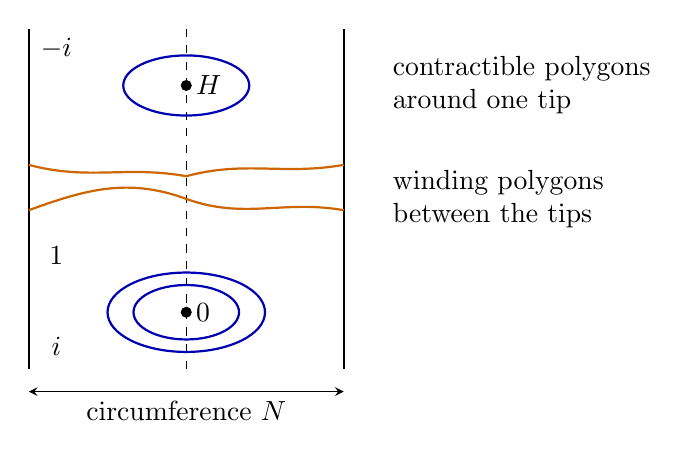
\begin{tikzpicture}[x=1cm,y=.72cm,>=stealth]
\draw[thick] (0,0)--(0,6) (4,0)--(4,6);
\draw[dashed] (2,0)--(2,6);
\fill (2,1) circle(2pt) node[right] {$0$};
\fill (2,5) circle(2pt) node[right] {$H$};
\node at (.35,.4) {$i$};
\node at (.35,2) {$1$};
\node at (.35,5.65) {$-i$};
\draw[blue!70!black,thick] (2,1) ellipse(.67 and .48);
\draw[blue!70!black,thick] (2,1) ellipse(1 and .7);
\draw[blue!70!black,thick] (2,5) ellipse(.8 and .53);
\draw[orange!80!black,thick] (0,2.8) to[out=20,in=160] (2,3) to[out=-20,in=170] (4,2.8);
\draw[orange!80!black,thick] (0,3.6) to[out=-15,in=170] (2,3.4) to[out=15,in=190] (4,3.6);
\draw[<->] (0,-.4)--(4,-.4) node[midway,below] {circumference $N$};
\node[align=left,anchor=west] at (4.5,5) {contractible polygons\\around one tip};
\node[align=left,anchor=west] at (4.5,3) {winding polygons\\between the tips};
\end{tikzpicture}
\caption{A schematic fundamental rectangle for the cylinder: its vertical sides are identified. The dashed seam has tips at cuts $0$ and $H$; the labels $i$, $1$, and $-i$ give its twist in the three row regions. The surviving contractible polygons enclose one tip, and the surviving winding polygons separate the tips. Dividing by the winding growth retains the two tip contributions. Curves are schematic and do not represent individual lattice edges.}
\label{fig:seam}
\end{figure}


The factor two between these exponents has a geometric meaning. When the seam tips are far apart, each tip supports a planar nest, while the winding polygons lie between them. The transfer coefficient records the two tip contributions after the extensive winding growth $\lambda_N^H$ has been removed. Proving this comparison requires height bounds: a cylinder polygon can be too tall, or its planar lift too wide, to belong to a small neighbourhood of one tip. We establish moments of every fixed order before making the projection.

\subsection{A complete route through the argument}

The proof begins with positive path sums. Section~\ref{sec:local} proves the local matrix identities, and Section~\ref{sec:cylinder} converts them into two estimates: a cylinder boundary deficit of order $N^{-1/4}$ and winding-polygon mass of order $N^{-1}$ per highest row. The deficit is the eventual source of the chord normalization $R^{3/4}$.

Sections~\ref{sec:vacuum}--\ref{sec:repeated-moments} determine the coefficient selected by the two caps. We first construct their normalized vectors and their polynomial denominator. A scalar residue formula then expresses products of row transfers between the caps, with an explicit normalization for the empty product. The root twists are initially independent. Resolving collisions proves that the scalar trace is holomorphic near a generic common twist, where colliding roots may contribute derivatives as well as ordinary evaluations. Adding and removing fused pairs of sites then extends the identity from distinct site arguments to arbitrary repeated row arguments by meromorphic continuation. This step is needed to compute powers $T^H$, not just a finite collection of special matrix elements.

Sections~\ref{sec:counting}--\ref{sec:asymptotics} identify the physical term in that formula. A real counting system has a unique branch in explicit quantile boxes, including the two extreme roots. Polynomial orthogonality identifies the vacuum end of the branch. Positivity of the finite annular transfer and a separate estimate on the two boundary caps select its ordinary residue coefficient at generic parameters. The finite annular gap and cap estimate make the selected coefficient analytic near each point of this real branch, so the identity continues to the homogeneous physical endpoints. The coefficient is a ratio $W/J$ of a root product and a Jacobian determinant, normalized at zero winding fugacity. Its logarithmic asymptotics give the exponent $1/6$.

Section~\ref{sec:projection} obtains arbitrary fixed height moments from higher twist derivatives, projects the cylinder polygons to the plane, and proves Theorem~\ref{thm:amplitude}. Section~\ref{sec:chords} completes the positive walk argument. An edge-slit exploration compares the weight of chords visiting an interior contact with the surrounding polygon partition. That contact weight is at most $R^{1/12+o(1)}$ everywhere and has this order throughout a central region. Summing order $R^2$ contacts gives the unnormalized length mass $R^{25/12+o(1)}$. The boundary deficit gives $Z_R^{\rm chord}\asymp R^{3/4}$, and their ratio is the exponent in Theorem~\ref{thm:triangle}.

The angle $l=\pi/8$ is fixed throughout; integer shifts inside bracketed trigonometric formulas denote multiples of $l$, whereas geometric row heights are integers in the physical lattice.

\section{Local transfer matrices and fusion}\label{sec:local}

We first describe the operator for one tile and prove its two rank reductions, its inverse relation, and its interchange identity. The resulting row identities will let us change the number and order of site parameters while keeping control of the transfer matrix.

The local algebra belongs to the integrable dilute-loop tradition. Grimm and Pearce~\cite{GrimmPearce1993} give a braid--monoid construction of dilute Yang--Baxter operators and explain their gauge equivalence with the Izergin--Korepin vertex model. We specify the gauge and scalar factors used here and verify the identities for the actual cap contractions.

\subsection{The local operator}

Set \(l=\pi/8,\ x=(2\cos l)^{-1},\ q=e^{2il},\ p=q^{-1}\). Let \(V\) have basis \(|m\rangle\), \(m=0,+1,-1\), with \(s|m\rangle=m|m\rangle\). The state \(0\) is vacant and the states \(\pm1\) are occupied. All transposes below are taken in these bases, without complex conjugation. Put \(C=\sum_{m=\pm1}p^m|m,-m\rangle\) and \(P|mk\rangle=|km\rangle\), and define the five scalar weights by
{\small
\[
 (a,b,h,d,e)(t)=
 \frac{(\sin2l\sin(3l-t),\,\sin2l\sin t,\,\sin(3l-t)\sin t,\,
 \sin(3l-t)\sin(2l-t),\,\sin(t-l)\sin t)}{\sin(2l+t)\sin(3l+t)} .
\]
}
Define \(R(t):V^{\otimes2}\to V^{\otimes2}\) by the following rules, where \(m,k=\pm1\) and the scalar weights have argument \(t\):
\[
 \begin{split}
 |00\rangle&\mapsto |00\rangle+b C,\qquad
 |m0\rangle\mapsto h|m0\rangle+a|0m\rangle,\quad |0m\rangle\mapsto h|0m\rangle+a|m0\rangle,\\
 |mk\rangle&\mapsto d|km\rangle+{\bf1}_{m=-k}p^{-m}(b|00\rangle+eC).
 \end{split}
\]
The rules conserve \(s_1+s_2\). Write \(\check R=R P\).

\subsection{Rank reductions and inversion}

At the two arguments \(2l\) and \(3l\), the range of \(R\) comes from a smaller space. For \(r=2\), let \(E=E_2:V\to V^{\otimes 2}\) take \(|0\rangle\) to \(|00\rangle+xC\) and \(|m\rangle\) to \(x(|m0\rangle+|0m\rangle)\) for \(m=\pm1\). For \(r=3\), let \(E=E_3:\mathbb C\to V^{\otimes 2}\) take 1 to \(|00\rangle+C\). The rank reduction and its compatible action on a third site are
\[
 R(rl)=EE^t P,\quad
 R_{23}(t)R_{13}(t+rl)(E\otimes I)=(E\otimes I)S,\quad S=
 \begin{cases}R(t+l)&r=2,\\I&r=3.\end{cases}
\]
Here \(S\) acts on the source of \(E\) and the third site; for \(r=3\) it is the identity on that third site. We also have the inverse relation \(R_{12}(t)R_{21}(-t)=I\). All these are meromorphic identities in their arguments.

To verify the rank reductions, substitute \(t=rl\) in the five weights and use \(C^t C=0\). We give the coefficient checks for the compatible action, since its scalar normalization will be used later. Use subscripts \(0,j,*\) for the arguments \(t,t+rl,t+l\). For \(r=2\), expand both sides on the inputs \(|00\rangle,|m0\rangle,|0m\rangle,|mk\rangle\) of \(V\otimes V\). The resulting coefficient equalities are grouped in that order in the following table:
\[
\begin{array}{ll}
 b_0+x a_jd_0=x b_*,& b_j a_0+x h_j h_0=x,\quad b_j h_0+x h_j a_0=x b_*;\\
 h_j+b_j b_0=h_*,&h_j b_0+b_j e_0=0,\quad a_j a_0+h_0=h_*,\\
 x(a_jh_0+a_0)=a_*,&b_j d_0=a_*;\\
 h_j h_0+x b_j a_0=h_*,& h_j a_0+x b_j h_0=x a_*,\quad a_j+x e_j b_0=x a_*,\\
 e_j d_0=h_*,& a_j b_0+x d_j d_0+x e_j e_0=0;\\
 d_j h_0+a_j a_0=d_*,&d_j a_0+a_j h_0=0,\quad h_j d_0=d_*,\\
 x(h_j b_0+b_j)=b_*,& b_j b_0+h_j e_0=e_*,\quad e_j a_0=b_*,\quad e_j h_0=e_* .
\end{array}
\]
The four groups occupy \(1,2,2,2\) rows. For example, the first group compares the three output types \(\sum p^m|0m,-m\rangle,\ \sum p^m|m,-m,0\rangle,\ \sum p^m|m0,-m\rangle\) on input \(|00\rangle\); the extra cap terms vanish because \(p^2+p^{-2}=0\). Each scalar equality follows on inserting the fractions and using \(2\sin A\sin B=\cos(A-B)-\cos(A+B)\) and \(8l=\pi\). For \(r=3\), the same substitution leaves the first and third groups, with the explicit \(x=h_*=1,\ a_*=b_*=0\); these are the required identities when site 3 is vacant and occupied, respectively.

The inverse relation reduces in the same way to
\[
 dd^-=1,\quad aa^-+hh^-=1,\quad ah^-+ha^-=0,\quad b+d b^-=0,\quad
 b b^-+d e^-+e d^-=0,
\]
where a superscript minus denotes the argument \(-t\). Direct substitution proves all five equalities.

\subsection{Interchange and row identities}

We next derive the interchange identity from the two rank reductions. Transpose the fusion relation and then conjugate by the operation reversing all spins. This combined operation leaves \(R\) unchanged, while spin reversal takes \(E\) to \(PE\). It therefore gives the opposite-product intertwining with \(E^t P\). Combining the two intertwinings with \(R(rl)=EE^tP\) proves
\[
 R_{12}(u-v)R_{13}(u)R_{23}(v)=R_{23}(v)R_{13}(u)R_{12}(u-v)
\]
when \(u-v=rl\), \(r=2,3\). It also holds at \(u-v=0\), since \(R(0)=P\). Multiplication by the inverse for the \(23\) pair identifies this equation with the \(132\) relation at differences \(u,u-v,-v\). The same three special cases therefore prove it when \(u=0,2l,3l\).

These six specializations determine the identity for every \(u\). Indeed, after clearing denominators, the powers of \(e^{iu}\) in each entry range from \(-4\) to \(4\) and have one parity: changing \(u\) by \(\pi\) conjugates by the sign of occupation at site 1. After removing a monomial factor, an entry is therefore a polynomial of degree at most four in \(e^{2iu}\). For generic \(v\), the six specializations are distinct modulo \(\pi\), so interpolation makes every entry zero. Meromorphic continuation gives the asserted identity for all parameters.

For a list of labelled site parameters \(\mathbf b=(b_1,\ldots,b_N)\) and \(\zeta\in\mathbb C^*\), define the spin row transfer by
\[
 T^\zeta(u;\mathbf b)=\operatorname{Tr}_a\big(\zeta^{s_a} R_{a1}(u-b_1)\cdots R_{aN}(u-b_N)\big).
\]
For a fixed twist \(\zeta\), these operators commute at all regular row arguments. To see this for \(N>0\), conjugate the trace over two auxiliary spaces by their \(R\), then use interchange at each site and conservation of the auxiliary spins. The same assertion holds for the empty list with the evident convention. Interchange also gives the adjacent exchange relation
\[
 T^\zeta(u;\ldots,A,B,\ldots)\check R_{j,j+1}(A-B)
 =\check R_{j,j+1}(A-B)T^\zeta(u;\ldots,B,A,\ldots).
\]
The analogous cyclic operation is as follows. Rotate the tensor factors one place to the left and multiply by \(\zeta^{s_1}\) on the site sent to the end. This map intertwines the row with the cyclically rotated list, by conservation in slot 1 and cyclicity of the auxiliary trace for entries at separate sites. Shifting a site parameter by \(\pi\) conjugates the row by the sign of occupation at that site.

Finally, specialize adjacent entries to \(d_0+rl,d_0\). The row intertwines through \(E_r\) with the shorter list obtained by replacing this pair with \(d_0+l\) for \(r=2\), or by deleting it for \(r=3\). This follows by inverting the fusion identity with site 3 as the auxiliary space and \(t=d_0-u\). The row relations, like the local ones, are meromorphic identities in all parameters.

\section{Positive boundary mass and winding polygons}\label{sec:cylinder}

We prove two estimates with constants uniform in the circumference: a
boundary deficit of order \(N^{-1/4}\), and a mass of order \(N^{-1}\)
for one winding polygon whose highest row is fixed.  The first step is
to prove that the boundary sums over all depths are finite.  We then
express the mass of one polygon as a polynomial in a tile weight, constrain that
polynomial by fusion, and recover both estimates from a strip integral.

Retain \(l=\pi/8\) and \(x=(2\cos l)^{-1}\), and put \(c=3/8\).
Orient the unit triangular tiling with horizontal sides.  A boundary
port is the midpoint of a triangle side.  A port-to-port path visits
each triangle at most once and joins two distinct side midpoints through
its centre; a path visiting \(m\) centres has weight \(x^m\).
For an integer \(g>0\), let \(K_\infty(g)\) be the total weight of
paths in the lower half-plane from horizontal boundary port \(0\) to
port \(g\).  In the quotient by horizontal translation by an integer
\(N\ge1\), let \(K_N(g)\), \(1\le g<N\), be the corresponding sum over
paths that are self-avoiding in the quotient and whose chosen lift has
endpoints \(0,g\).  In particular, \(K_N(g)\le K_\infty(g)\).
All domain boundaries and row cuts in this section follow triangle
sides.

Group the triangles into rows of \(\pi/3\)-rhombi, with sides parallel
to \(0\) and \(\pi/3\); the row index increases by one under translation
by \(e^{i\pi/3}\).  Let \(P_N\) be the sum of \(x^{|\gamma|}\) over
simple noncontractible polygons in the infinite quotient cylinder
whose highest occupied row is a specified row.  Here \(|\gamma|\) is
the number of visited centres, equivalently the number of polygon
edges.  Each actual quotient polygon is counted once without
orientation.  Thus \(P_N\) is a bare sum of single-polygon weights; it
will be the derivative at winding fugacity zero, with no factor two.

\begin{proposition}[Cylinder deficit and winding mass]\label{prop:cylinder}
In these port and highest-row conventions,
\[
 D_N:=1-2\cos(3l)\sum_{g=1}^{N-1}K_N(g)\asymp N^{-1/4},
 \qquad
 P_N\asymp N^{-1}.
\]
The comparison constants can be chosen independently of the integer
circumference \(N\ge1\).
\end{proposition}

\subsection{Finite boundary flux and half-plane summability}

Consider a convex finite domain tiled by triangles, and fix an entrance
port \(a\).  Give a path of total signed turn \(W\) the complex weight
\(e^{icW}x^m\).  The sum of these weights over paths from \(a\) to all
exit ports is \(1\).  We recall the local cancellation, including its
phases, because the sign changes when the source lies in an interior
slit later in the paper.

Introduce one unit of inward flux at \(a\), and stop a partial path
whenever it reaches a side midpoint, recording whether it points into
a triangle or out of one.  At a fresh triangle the two extensions turn
by \(\pm\pi/3\).  Their total multiplier is
\[
 2x\cos(c\pi/3)=1.
\]
At a previously visited triangle, pair the two stopped paths obtained
by reversing the cycle segment.  To check their phases, suppose that
the earlier arrival-to-exit turn was \(+\pi/3\).  The closing turn of
the cycle is then \(-\pi/3\).  The prefix from the boundary source
arrives from the exterior of that cycle, so the cycle has rotation
\(-2\pi\): in the counterclockwise alternative the reflex interior
sector would contain the arriving prefix.  Including the earlier turn
gives a net increment \(-4\pi/3\), which becomes \(+4\pi/3\) on
reversal.  The pair cancels because
\[
 2\cos(4\pi c/3)=0.
\]
The reflected case has the same cancellation.  Thus all interior
stops cancel and the input flux equals the boundary output.

For an exit port \(b\) following \(a\) counterclockwise, let
\(\phi_a,\phi_b\) be the lifted counterclockwise boundary tangents.
Closing the path along the boundary gives
\[
 W=\phi_b-\phi_a-\pi.
\]
Convexity puts \(W\) in \([-\pi,\pi]\), so every real output weight is
positive.  Exhaust the lower half-plane by increasing triangles
symmetric about \(a\).  The two directions along their horizontal
base have phases \(e^{\pm ic\pi}\), both with real part
\(\cos(3l)\).  Monotone convergence for these base paths, with the
other positive exits discarded, gives
\begin{equation}\label{eq:cyl-half-plane}
 2\cos(3l)\sum_{g>0}K_\infty(g)\le1.
\end{equation}
This finite bound is the input for the annular cap construction.  The
equality and the endpoint tail estimate will follow after the deficit
has been evaluated.

\subsection{Annular diagram rows and the zero-fugacity cap}

We first distinguish the two row operators that enter the argument.
The spin row \(T^\zeta(u;\mathbf b)\) of Section~\ref{sec:local} acts on
\(V^{\otimes N}\), with a twist \(\zeta^{s_a}\) in the auxiliary trace.
The diagram row defined below acts instead on annular arch patterns.
The two descriptions give the same scalars when the open diagram ports
are closed with the specified caps and the orientations are summed;
we do not identify their state spaces.

A tile has two incoming legs, auxiliary from the right and quantum
from below, and the opposite outgoing legs.  Its scalar weights are
the functions \(a,b,h,d,e\) of Section~\ref{sec:local}.  An empty tile
has weight \(1\).  A single connection from one input to the other
stream's output has weight \(a\), a single straight connection has
weight \(h\), and a cup or cap joining the two inputs or the two
outputs has weight \(b\).  When all four legs are occupied, the
double pairing of \(a\)-type has weight \(d\), and the other double
pairing has weight \(e\).  Contractible closed loops have weight zero,
and simple winding loops have weight \(n\).  At the physical argument
\(t=l\),
\[
 (a,b,h,d,e)(l)=(x,x^2,x^2,x^2,0).
\]
These are exactly the weights of dual self-avoiding paths in the two
triangles of a split rhombus.

Here is the orientation comparison with the spin matrix.  Choose
\(\zeta\ne0\) with \(n=\zeta+\zeta^{-1}\) and orient each occupied
arc.  The spins \(+1,-1\) mean respectively along and against the
positive stream direction.  Straighten the positive stream tangents
at the tile ports to parallel forward directions, with the auxiliary
stream to the right of the quantum stream at entry and to its left
at exit.  A through connection then has net turn zero.  A clockwise
cup or cap has phase \(p=e^{-i\pi/4}\), and a counterclockwise one has
phase \(p^{-1}\), exactly as in the terms involving \(C\) and
\(p^{-m}\) in \(R(t)\).  These spin phases use one quarter of the turn
angle, separately from the boundary flux phase \(e^{icW}\) above.
The changes of tangent used in straightening cancel at each join, so
a closed curve of signed rotation \(\Theta\) has phase
\(e^{i\Theta/4}\).  Equivalently, the phase counts signed cups and
caps and is unchanged by isotopy fixing the port tangents.

A contractible simple loop has rotation \(\pm2\pi\); its two
orientations therefore contribute \(i\) and \(-i\), with sum zero.
A simple winding loop has rotation zero in the flat cylinder frame
and seam flux \(\pm1\); its orientation sum is
\(\zeta+\zeta^{-1}=n\).  This remains true for a diagram closed by
arches in earlier rows.  For each such arch one chooses an actual
representative below the row, with the prescribed port tangents and
homotopy, and includes that representative's own turn and seam
factors.  Representatives above a row are handled in the same way.

We also need the interchange and inversion identities with open
connections.  For interchange, place streams \(1,2,3\) from right
to left at entry, all pointing forward, and in reverse order at exit.
For fixed occupied boundary slots in a disk, the
oriented tensors of distinct noncrossing matchings are linearly
independent.  Indeed, after straightening the port tangents, the
nonzero arc phase depends only on the oriented connectivity.  For a
chosen matching, assign inward spins to its left endpoints and outward
spins to its right endpoints in a linearized boundary order.  The
result is a Dyck word.  At every gap, a matching compatible with this
assignment has at least the Dyck height many open arcs; equality at
every gap singles out the chosen matching.  Ordering matchings by
these height tests gives a triangular test matrix with nonzero
diagonal.  The spin identities of Section~\ref{sec:local} therefore
imply the corresponding identities of open diagrams.

Sliding a crossing of two auxiliary streams around the \(N\) sites
now proves commutation of periodic diagram rows: insert the crossing
and its inverse, use interchange at each site, and cancel them after
the trace.  Any loops formed during this operation are annular loops
with the prescribed weights.  The proof applies at generic regular
parameters and extends as a meromorphic identity.

Write \(\mathsf T_n(t)\) for the homogeneous diagram row with argument
\(t\) and winding weight \(n\).  A state specifies, at the bottom
boundary circle, which of the \(N\) slots are vacant and how the
occupied slots are joined by noncrossing arches below the circle,
including their homotopy classes.  No strand runs to infinity.
A chosen lift of each arch has endpoint span of absolute value less
than \(N\), since an arch disjoint from its translates cannot have
interlacing lifted endpoints.  There are consequently only finitely
many states.  To act by \(\mathsf T_n(t)\), attach a row above the
input arches, evaluate closed loops, and read the output arch pattern.
The preceding diagram interchange gives, for the same winding weight,
\[
 \mathsf T_n(u)\mathsf T_n(v)=\mathsf T_n(v)\mathsf T_n(u).
\]

Let \(|0\rangle\) be the all-vacant state and let \(\langle0|\) select
its component.  Set \(T(t):=\mathsf T_0(t)\), retaining this shorthand
for the zero-fugacity diagram row.  Every nonempty configuration with
empty output contains a closed loop, so
\[
 \langle0|T(t)=\langle0|.
\]
We next prove, for each fixed \(N\),
\begin{equation}\label{eq:cyl-cap-limit}
 T(l)^H\longrightarrow|\Psi\rangle\langle0|
 \qquad(H\to\infty),\qquad \langle0|\Psi\rangle=1.
\end{equation}

\paragraph{Empty input.}
The column \(T(l)^H|0\rangle\) is the positive sum of physical arch
systems of depth at most \(H\).  For a fixed output pattern, lift each
component path to the half-plane.  Its endpoint separation has
absolute value less than \(N\), and its total weight is bounded by
the corresponding \(K_\infty(g)\).  Ignoring mutual avoidance bounds
the arch-system sum by products of these finite masses.  Only
finitely many endpoint and homotopy choices occur at fixed \(N\).
Thus each component increases to a finite limit.  These limits define
the finite vector \(\Psi\); its empty component is \(1\).

\paragraph{Nonempty input.}
Fix a nonempty annular pattern \(\alpha\).  It has a physical
realization of positive weight in finitely many rows below the cut.
To construct one, repeatedly choose a pair whose bounded disk side
contains no endpoints still to be joined.  Cap that pair across its
auxiliary interval, using one \(a\), one \(b\), and the intervening
\(h\)'s in bottom-to-top notation, while carrying all other
occupations straight.  This also permits an interval crossing the
seam.  The construction terminates, and all its weights at \(l\)
are positive.

Attach this one fixed realization beneath a diagram counted by the
column \(T(l)^H|\alpha\rangle\).  The union determines the original
bulk diagram, so this attachment is injective.  At zero fugacity no
closed component survives.  Hence every segment belongs to an output
arch, and at least one such arch reaches the attached realization,
at depth at least \(H-O_\alpha(1)\).  The output weight multiplied by
the fixed positive cap weight is therefore bounded by the tail of the
convergent sum of completed arch systems.  That tail tends to zero.  Every
nonempty input column thus tends to zero, proving
\eqref{eq:cyl-cap-limit} in the finite state space.

Commutation and the left empty identity now give the common right
fixed vector:
\[
 T(t)|\Psi\rangle\langle0|
   =\lim_{H\to\infty}T(l)^H T(t)
   =|\Psi\rangle\langle0|T(t)
   =|\Psi\rangle\langle0|,
 \qquad T(t)\Psi=\Psi.
\]
The limit \eqref{eq:cyl-cap-limit} also says that \(1\) is a simple
eigenvalue of \(T(l)\), with all remaining eigenvalues strictly inside
the unit disk; the principal nonempty block has spectral radius less
than \(1\).  These are fixed-\(N\) conclusions.  They give a locally
analytic eigenpair under a small change of winding fugacity at each
fixed \(N\), as used for the higher derivatives in
Section~\ref{sec:projection}, but give no uniform spectral gap or
uniform analyticity radius in \(N\).

\subsection{The one-winding derivative, fusion, and its polynomial}

Keep the cap \(\Psi\) at zero fugacity and define
\begin{equation}\label{eq:cyl-bare-J}
 J_N(t):=
 \left\langle0\left|
       \left.\partial_n\mathsf T_n(t)\right|_{n=0}
 \right|\Psi\right\rangle .
\end{equation}
The derivative selects exactly one winding loop closed by the new
row: \(\partial_n n|_{0}=1\), while higher powers of \(n\) vanish.
The cap below contains ordinary open arches and no closed loops.
At \(t=l\) the new row is the unique highest occupied row of the
resulting polygon.  Thus each actual unoriented quotient polygon is
counted once, without a marked vertex or a division by horizontal
translations, and
\[
 J_N(l)=P_N.
\]
The fugacity-\(2\) gas used later instead assigns \(2x^{|\gamma|}\)
to each polygon.

\paragraph{Fusion after closing the caps.}
For any fixed annular bottom cap \(\alpha\), the local fusion identity
implies a scalar relation before differentiation:
\begin{equation}\label{eq:cyl-capped-fusion}
 \left\langle0\left|
   \mathsf T_n(t)\mathsf T_n(t+2l)-\mathsf T_n(t+l)
 \right|\alpha\right\rangle
 =t^N R_\alpha(t,\zeta),
 \qquad n=\zeta+\zeta^{-1},
\end{equation}
where \(R_\alpha\) is analytic near \(t=0,\zeta=i\).
To see the order \(N\), label the two auxiliary spaces \(1,2\).
The local product
\(R_{23}(t)R_{13}(t+2l)\) preserves
\(E_2V\otimes V_3\) and acts there as the single tile \(R(t+l)\).
Moreover, \(E_2\) intertwines \(\zeta^{s_1+s_2}\) with
\(\zeta^s\), so the trace on that subspace is the fused row.  On the
quotient auxiliary space, each local product is \(O(t)\): at \(t=0\)
it is \(P_{23}R_{13}(2l)\), whose range already lies in
\(E_2V\otimes V_3\).  Its product around \(N\) sites is therefore
\(O(t^N)\).  Closing with the chosen oriented representative of
\(\alpha\), including its turn and seam factors, converts this spin
trace relation to \eqref{eq:cyl-capped-fusion}.

There are finitely many cap patterns, each with a finite coefficient
in \(\Psi\), so \eqref{eq:cyl-capped-fusion} also holds with
\(\alpha\) replaced by \(\Psi\).  Near \(\zeta=i\), the quantity
\(n=\zeta+\zeta^{-1}\) is a local analytic coordinate because
\(dn/d\zeta=2\) there.  Differentiate that scalar relation at \(n=0\),
with the cap coefficients fixed.  The identities
\(T(t)\Psi=\Psi\) and \(\langle0|T(t)=\langle0|\) reduce the two
derivatives of the product to \(J_N(t)\) and \(J_N(t+2l)\).  Hence
\begin{equation}\label{eq:cyl-differentiated-fusion}
 J_N(t)+J_N(t+2l)-J_N(t+l)=O(t^N)
 \qquad(t\to0).
\end{equation}
No derivative of \(\Psi\) is taken in this argument.

\paragraph{Dependence on the straight weight.}
At empty output, a full horizontal auxiliary loop contributes
\(h(t)^N\) once.  Otherwise the occupied auxiliary intervals have
positive integer lengths \(s_1,\ldots,s_r\) and alternate with gaps
of positive lengths \(g_1,\ldots,g_r\).  Their bottom endpoints are
paired by arches in \(\Psi\).  We claim that each such arch crosses
one consecutive gap.

Indeed, in the lift an arch cuts off a bounded disk side.  It encloses
an even number of other endpoints, so its two endpoints are of
opposite types in the alternating list of interval starts and ends.
The incident row intervals therefore both point into that disk side
or both point out.  The first case closes a component inside the
bounded lifted disk.  In the second case, any enclosed endpoints are
paired internally both by arches and by row intervals, again making
a closed component inside that disk.  Such components are
contractible on the cylinder and have zero weight.  The disk side must
therefore contain no other endpoint, which is precisely a pairing
across a consecutive gap.

Put \(C_0=2\cos(3l)\).  The local weight formulas give, for each
occupied interval,
\[
 a(t)b(t)h(t)^{s_i-1}=C_0(1-h(t))h(t)^{s_i}.
\]
A labelled cyclic arrangement \(\mathcal A\) records its actual
intervals on the \(N\)-site ring and the resulting arches across the gaps;
write \(\Psi(\mathcal A)\) for that pattern's cap mass.  Consequently
\[
\begin{aligned}
 J_N(t)&=f_N(h(t)),\\
 f_N(u)&=u^N+
   \sum_{\mathcal A}
     C_0^{\,r}(1-u)^r u^{s_1+\cdots+s_r}\Psi(\mathcal A).
\end{aligned}
\]
Each actual labelled arrangement is counted once, with no additional
marked starting site.
The lengths satisfy \(\sum_i(s_i+g_i)=N\), so
\(r+\sum_i s_i\le N\).  Thus \(f_N\) is a polynomial of degree at
most \(N\) and \(f_N(1)=1\).  At first derivative order at \(u=1\),
only the full ring and the one-interval terms survive.  For a gap of
length \(g\in\{1,\ldots,N-1\}\), the one interval has \(N\) labelled
starting positions, its cap mass is \(K_N(g)\), and the derivative of
\((1-u)u^{N-g}\) at \(1\) is \(-1\).  We have proved the exact
normalization
\begin{equation}\label{eq:cyl-polynomial}
 \deg f_N\le N,\qquad
 f_N(1)=1,\qquad
 f_N'(1)=N-C_0N\sum_{g=1}^{N-1}K_N(g)=ND_N.
\end{equation}

\subsection{The strip operator}

Use the strip coordinate \(s=2t-3l\), and write
\[
 \alpha_{\rm s}:=\frac{\pi}{6l}=\frac43,\qquad
 \beta_{\rm s}:=\alpha_{\rm s}^{-1}=\frac34,\qquad
 S_a:=\{s\in\mathbb C:|\Re s|<a\}.
\]
The local straight weight in this coordinate is
\[
 h(t)=\frac{\cos s-\cos3l}{\cos s+\cos l}
 \quad\text{when }s=2t-3l.
\]
Define
\[
 j(s):=f_N\left(\frac{\cos s-\cos3l}{\cos s+\cos l}\right),
 \qquad
 G(s):=j(s-2l)+j(s+2l)-j(s).
\]
Then \(j(2t-3l)=J_N(t)\), and
\(G(2t-l)\) is the left side of
\eqref{eq:cyl-differentiated-fusion}.  Both \(j\) and \(G\) are even,
so \(G\) has zeros of order at least \(N\) at \(s=\pm l\).
Also \(j(i\infty)=G(i\infty)=1\).

The following representation depends only on the polynomial degree,
not on fusion.  This distinction will allow the same operator to be
used for higher winding derivatives.  For each fixed \(N\) and any
polynomial \(f\) of degree at most \(N\), put
\[
 j_f(s)=f\left(\frac{\cos s-\cos3l}{\cos s+\cos l}\right),
 \qquad
 G_f(s)=j_f(s-2l)+j_f(s+2l)-j_f(s).
\]
Define the even map and the convolution
\[
 B(s):=\frac{\cos(\alpha_{\rm s}s)-d_0}
             {\cos(\alpha_{\rm s}s)+d_0},
 \qquad d_0:=\cos(\alpha_{\rm s}l)=\frac{\sqrt3}{2},
 \qquad
 (\mathcal C_g F)(s):=\int_{\mathbb R}g(y)F(s+iy)\,dy,
\]
\[
 g(y):=\frac1{2\pi}
 \left(\frac{2^{-1/2}}{\cosh y-2^{-1/2}}-\frac1{\cosh y}\right).
\]
The map \(B\) identifies the quotient of \(S_{3l}\) by \(s\mapsto-s\)
conformally with the disk.  It sends \(\pm l\) to \(0\), and
\(B'(l)\ne0\).  The kernel \(g\) is real and even.  With
\(\widehat g(k)=\int g(y)e^{iky}\,dy\), residues over the \(2\pi i\)
period give
\[
 1-\widehat g(k)
 =1-\frac{\sinh(6lk)-\sinh(4lk)}{\sinh(8lk)}
 =(2\cosh(2lk)-1)\frac{\sinh(6lk)}{\sinh(8lk)}.
\]
The expressions at \(k=0\) are interpreted by continuity.
Furthermore,
\[
 \int_{\mathbb R}g=\frac14,\qquad p_g:=\int_{\mathbb R}|g|<\frac12.
\]
For the strict inequality, the negative part is zero on \(|y|\le1\)
and is bounded by
\((1-2^{-1/2})/(2\pi\cosh y)\) on \(|y|>1\); integrating this bound
and adding twice the negative mass to \(1/4\) gives \(p_g<1/2\).

With these definitions, the degree bound gives the representation
\begin{equation}\label{eq:cyl-strip-representation}
\begin{gathered}
 G_f(s)=(I-\mathcal C_g)q(B(s))+\lambda
 \quad(s\in S_{3l}),\\
 q(z)=\sum_{m=1}^N q_mz^m,
\end{gathered}
\end{equation}
for some \(q\) and constant \(\lambda\).

To prove \eqref{eq:cyl-strip-representation}, first Fourier transform
\(j_f(iy)-f(1)\), which decays exponentially at both ends.  Shifting
the contour through one real period \(16l\) crosses the mirrored poles
at \(7l,9l\), each of order at most \(N\).  Their residues give, on
\(S_{7l}\),
\[
 j_f(s)=f(1)+\int_{\mathbb R}
       \frac{H(k)}{\sinh(8lk)}e^{ks}\,dk,
 \qquad
 H(k)=P_e(k)\sinh(lk)+P_o(k)\cosh(lk),
\]
where \(P_e\) is even, \(P_o\) is odd, and both have degree at most
\(N-1\).  The displayed symbol therefore gives
\[
 G_f'=(I-\mathcal C_g)F,\qquad
 F(s):=\int_{\mathbb R}\frac{kH(k)}{\sinh(6lk)}e^{ks}\,dk.
\]

Here \(F\) lies in the holomorphic odd Bergman space on \(S_{3l}\),
with area norm \(\int_{S_{3l}}|F|^2\,dA\).  This space explains the
degree bound in \eqref{eq:cyl-strip-representation}.  Plancherel on
the vertical lines \(s=r+iy\), followed by integration over
\(-3l<r<3l\), gives the Fourier-side norm multiplier
\(\sinh(6lk)/k\), up to the Fourier normalization.  The line
transforms satisfy
\(\partial_r\widehat F=k\widehat F\) on interior lines in the sense
of distributions, by the Cauchy--Riemann equation.  In this norm the
span of the representers for jets of orders \(0,\ldots,N-1\) at \(l\),
restricted to odd functions, consists exactly of the preceding
numerators \(kH(k)\): even jet orders give the \(\sinh(lk)\) terms
and odd orders the \(\cosh(lk)\) terms.

Equivalently, every odd holomorphic function on the strip has an even
primitive, which is a function of \(B\).  For a primitive
\(p(B(s))\) with \(p(z)=\sum_{n\ge1}p_nz^n\), conformal change of
variables gives
\[
 \int_{S_{3l}}|(p(B))'|^2\,dA
       =2\pi\sum_{n\ge1}n|p_n|^2.
\]
This parametrizes the whole odd Bergman space.  Since \(B'(l)\ne0\),
the jets of \(F=(p(B))'\) of orders \(0,\ldots,N-1\) at \(l\) are
triangularly equivalent to the first \(N\) coefficients of \(p\).
Their representer span is therefore exactly the set of \((q(B))'\)
with \(\deg q\le N\) and
\(q(0)=0\).  Thus \(F=(q(B))'\), and integration in \(s\) proves
\eqref{eq:cyl-strip-representation}.

For later use, express the convolution on these coefficients.
Because \(g\) is even, \(\mathcal C_g B^m\) is even and hence a
holomorphic function of \(z=B(s)\).  With the local inverse branch
\(s(0)=l\), set
\[
\begin{aligned}
 \Phi_m(z)&:=(\mathcal C_g B^m)(s(z)),&
 M_{nm}&:=[z^n]\Phi_m(z)\quad(n,m\ge1),\\
 M_{0m}&:=\Phi_m(0)=(\mathcal C_g B^m)(l).&&
\end{aligned}
\]
Since \(|B(l+iy)|<1\), the defining convolution also gives
\(|M_{0m}|\le p_g\).
The matrix \(M\) is real and self-adjoint on
\[
 \ell^2(n):=\left\{v:\sum_{n\ge1}n|v_n|^2<\infty\right\},
 \qquad \|M\|_{\ell^2(n)\to\ell^2(n)}\le p_g.
\]
Indeed \((\mathcal C_g B^m)'=\mathcal C_g(B^m)'\), so differentiation
identifies its action with \(\mathcal C_g\) on the odd Bergman space.
Imaginary translations are unitary on the
full strip Bergman space; their average against the real even kernel
is self-adjoint, has norm at most \(\|g\|_1\), and preserves oddness.
In particular,
\[
 nM_{nm}=mM_{mn}.
\]
This Hilbert-space contraction does not assert contraction on
\(\ell^1\).

Apply \eqref{eq:cyl-strip-representation} to the first-derivative
function \(G\).  Its order-\(N\) zero at \(B=0\) gives
\[
 q_n=\sum_{m=1}^N M_{nm}q_m\quad(1\le n<N),
 \qquad
 \lambda=\sum_{m=1}^N M_{0m}q_m.
\]
The compressed Hilbert contraction makes \(I-(M_{nm})_{n,m<N}\)
invertible.  Define its unique normalized solution by
\[
 Q_N(z):=\sum_{m=1}^N c_mz^m,\qquad
 c_N=1,\qquad c_n=\sum_{m=1}^N M_{nm}c_m\quad(1\le n<N).
\]
If \(q_N=0\), the contraction would force \(q=0\), and the zero at
\(l\) would force \(G=0\), contrary to \(G(i\infty)=1\).  Thus \(q\)
is a nonzero multiple of \(Q_N\).  For a polynomial with zero
constant coefficient define
\[
\begin{aligned}
 (\mathcal Tq)(s)&:=(I-\mathcal C_g)q(B(s))
                      +(\mathcal C_g q(B))(l),\\
 \mathcal E(q)&:=(\mathcal Tq)(i\infty)
       =\frac34q(1)+\sum_mM_{0m}q_m.
\end{aligned}
\]
Writing \(\widetilde G:=\mathcal TQ_N\) and
\(E_N:=\mathcal E(Q_N)\), we obtain
\begin{equation}\label{eq:cyl-normalized-G}
 E_N\ne0,\qquad G(s)=\frac{\widetilde G(s)}{E_N}.
\end{equation}
The nonvanishing here holds for each fixed \(N\), by the existing
function \(G\).  We next need bounds on this normalizer as \(N\)
varies.

\subsection{Uniform control of the normalizer}

The Hilbert contraction has determined \(Q_N\), but a two-sided
estimate for \(G\) requires a strict bound on its lower
coefficients.  The following estimates for \(M\) will give that bound.

\paragraph{Matrix entries.}
For one constant \(C\), independent of \(n,m\ge1\),
\begin{equation}\label{eq:cyl-M-bounds}
\begin{gathered}
 |M_{nm}|\le\frac Cn
   \min\left\{\left(\frac nm\right)^{\beta_{\rm s}},
              \left(\frac mn\right)^{\beta_{\rm s}}\right\},
 \\
 |M_{n+1,m}-M_{nm}|\le\frac C{n^2},
 \qquad
 |M_{0m}|\le C m^{-\beta_{\rm s}}.
\end{gathered}
\end{equation}
Here is a contour proof.  Choose a fixed \(0<\delta<l/2\),
independently of \(n,m\), and continue
\(\mathcal C_g B^m\) from \(S_{3l}\) to \(S_{3l+\delta}\) by moving
the \(y\)-contour by at most \(2\delta i\), so that the argument of
\(B\) stays in \(|\Re s|\le3l-\delta\).  The kernel is holomorphic
for \(|\Im y|<2l\), so no pole of \(g\) is crossed.
On these contours,
\[
 |g(y)|\le C e^{-|\Re y|},\qquad
 |B(s)|\le \exp(-c_1e^{-\alpha_{\rm s}|\Im s|})
 \quad (|\Re s|\le3l-\delta).
\]
As an even function of \(s\), the continuation descends through the
inverse branch point \(B(0)\) to a
\(z\)-domain containing, for some \(\epsilon>0\),
\[
 |z|<1+\epsilon,\qquad
 |\arg(1-z)|<\frac{\pi}{2}+\epsilon,\qquad z\ne1.
\]
Away from \(z=1\) this follows by compactness and the disk mapping.
Near \(1\), inversion of
\(\cos(\alpha_{\rm s}s)=d_0(1+z)/(1-z)\) gives both the continued
domain and
\(e^{-\alpha_{\rm s}|\Im s|}\asymp |1-z|\).  Consequently,
\[
 |\Phi_m(z)|
 \le C\int_{\mathbb R}e^{-|y|}
       \exp\!\left(-c_2m|1-z|e^{-\alpha_{\rm s}|y|}\right)\,dy
 \le C'\min\{1,(m|1-z|)^{-\beta_{\rm s}}\}.
\]

For sufficiently large \(n\), use Cauchy's coefficient contour with
outer radius \(1+\epsilon/2\), indented along
\(1-z=r e^{\pm i(\pi/2+\epsilon/2)}\) to \(r=1/n\), then along the
small circle of that radius.  On the rays,
\(|z|^{-n-1}\le C e^{-c n r}\), since their angle is greater than
\(\pi/2\); the small circle has length \(O(1/n)\) and bounded
\(|z|^{-n-1}\).  The preceding bound on \(\Phi_m\) therefore gives
\[
 |M_{nm}|\le\frac Cn\min\{1,(n/m)^{\beta_{\rm s}}\}.
\]
Applying the same contour to \((1-z)\Phi_m(z)\) gives the difference
bound in \eqref{eq:cyl-M-bounds}.  For the finitely many smaller
\(n\), use a fixed circle \(|z|=r_*<1\); there \(|1-z|\) is bounded
away from zero, so the bound on \(\Phi_m\) is uniform in \(m\) and
gives the same estimates after increasing \(C\).  The symmetry
\(nM_{nm}=mM_{mn}\) supplies the additional
\((m/n)^{\beta_{\rm s}}\) factor, and the bound at \(z=0\) gives the
stated estimate for \(M_{0m}\).

\paragraph{The mass of a high column.}
The entry and difference bounds also imply the sharper limit
\begin{equation}\label{eq:cyl-column-limit}
 \sum_{n\ge1}|M_{nm}|\longrightarrow p_g
 \qquad(m\to\infty).
\end{equation}
To prove it, consider the finite signed measures
\[
 \mu_m:=\sum_{n\ge1}M_{nm}\,\delta_{n/m}
 \quad\text{on }(0,\infty).
\]
The entry bound makes their total variations uniformly bounded and
tight in compact ratio ranges.  More precisely, the total variation
on \(n/m<\eta\) is \(O(\eta^{\beta_{\rm s}})\), and that on
\(n/m>R\) is \(O(R^{-\beta_{\rm s}})\), uniformly in \(m\).

For fixed \(a>0\) and all sufficiently large \(m\), choose
\(Y_m\to\infty\) so that
\(B(iY_m)=e^{-a/m}\).  For each fixed \(y\),
\[
 B(i(Y_m+y))^m\longrightarrow
       \exp(-a e^{-\alpha_{\rm s}y}).
\]
Since \(0<B(iu)<1\) for real \(u\), dominated convergence and
\(M_{0m}\to0\) show
\[
 \int e^{-au}\,d\mu_m(u)
 =\Phi_m(e^{-a/m})-M_{0m}
 \longrightarrow
 \int_{\mathbb R}g(y)\exp(-a e^{-\alpha_{\rm s}y})\,dy.
\]
This is the Laplace transform of the smooth pushforward of
\(g(y)\,dy\) by \(u=e^{-\alpha_{\rm s}y}\), whose density is
\[
 \rho(u)=\frac1{\alpha_{\rm s}u}
         g\!\left(-\frac{\log u}{\alpha_{\rm s}}\right).
\]
Tightness and uniqueness of Laplace transforms give weak convergence
to \(\rho(u)\,du\).  To pass from signed convergence to total
variation, interpolate the values \(mM_{nm}\) linearly at \(u=n/m\).
On each compact interval in \((0,\infty)\), the entry bound makes
these interpolants bounded and the difference bound makes them
equicontinuous.  Every locally uniform subsequential limit must be
\(\rho\): for a compactly supported continuous test function
\(\varphi\), the identity
\[
 \int\varphi\,d\mu_m
 =\frac1m\sum_n\varphi(n/m)\,[mM_{nm}]
\]
is a Riemann sum for the interpolant limit, and its weak limit is
\(\int\varphi(u)\rho(u)\,du\).  Thus the convergence is locally uniform.
The tight total-variation tails then give
\[
 \sum_{n\ge1}|M_{nm}|\longrightarrow
 \int_0^\infty|\rho(u)|\,du=\int_{\mathbb R}|g(y)|\,dy=p_g,
\]
which proves \eqref{eq:cyl-column-limit}.

\paragraph{The lower coefficients of \(Q_N\).}
Write \(c=c^{(N)}\) as a sequence by setting \(c_m=0\) for \(m>N\).
We claim
\begin{equation}\label{eq:cyl-c-margin}
\begin{gathered}
 \sup_N\|c^{(N)}\|_1<\infty,\qquad
 c_m^{(N)}\longrightarrow0\ \text{for every fixed }m,\\
 \limsup_{N\to\infty}\sum_{m<N}|c_m|
       \le\frac{p_g}{1-p_g}<1.
\end{gathered}
\end{equation}
The proof uses the Hilbert contraction for possible fixed mass and
\eqref{eq:cyl-column-limit} for mass escaping to high indices.

Suppose first that \(\|c^{(N)}\|_1\) is unbounded along a subsequence
with \(N\to\infty\).
Divide by that norm to obtain \(\|v^{(N)}\|_1=1\).  The recurrence
for \(c\), including \(c_N=1\), becomes
\[
 \left\|v^{(N)}-\mathbf1_{\{n<N\}}Mv^{(N)}\right\|_1\longrightarrow0.
\]
Pass to a coordinatewise limit \(v\in\ell^1\), using Fatou's lemma.
Every fixed row
\(M_{nm}\) tends to zero as \(m\to\infty\), by
\eqref{eq:cyl-M-bounds}; this lets the recurrence pass to the limit,
giving \(v=Mv\).  Also \(|v_n|\le C\|v\|_1/n\), so
\[
 \sum_n n|v_n|^2\le C\|v\|_1\sum_n|v_n|<\infty.
\]
The strict contraction on \(\ell^2(n)\) forces \(v=0\).

Let \(d_m:=\sum_n|M_{nm}|\).  The entry bound makes \(d_m\) uniformly
bounded, and \eqref{eq:cyl-column-limit} gives
\(d_m\le p_g+\varepsilon<1\) for all sufficiently large \(m\).
The approximate recurrence and \(v_m^{(N)}\to0\) at each fixed index
would then imply
\[
 1\le \sum_{m\le J}d_m|v_m^{(N)}|
       +(p_g+\varepsilon)\|v^{(N)}\|_1+o(1)
 \longrightarrow p_g+\varepsilon<1
\]
for a suitable fixed \(J\), a contradiction.  This proves the first
claim of \eqref{eq:cyl-c-margin}.  With bounded norms, the same
coordinatewise-limit argument applies directly to \(c^{(N)}\);
every limit is an \(\ell^2(n)\) fixed point of \(M\), hence zero.
This proves the second claim.

Finally the recurrence and the column norms give
\[
 \sum_{n<N}|c_n|\le\sum_{n\ge1}|(Mc)_n|
                 \le\sum_m d_m|c_m|.
\]
The contribution of any fixed initial set of columns tends to zero.
Given \(\varepsilon>0\), choose the remaining columns so that
\(d_m\le p_g+\varepsilon\), let \(N\to\infty\), and then let
\(\varepsilon\downarrow0\).  With
\(\|c\|_1=1+\sum_{m<N}|c_m|\), this yields
\[
 \limsup_N\sum_{m<N}|c_m|
 \le p_g\left(1+\limsup_N\sum_{m<N}|c_m|\right),
\]
which is the third claim of \eqref{eq:cyl-c-margin}.  The same split
also gives
\[
 \limsup_N\|Mc\|_1\le\frac{p_g}{1-p_g}<1.
\]

All coefficients are real.  Hence \eqref{eq:cyl-c-margin} makes
\(Q_N(1)=1+\sum_{m<N}c_m\) positive and bounded away from zero for
all sufficiently large \(N\).  Moreover
\(\sum_mM_{0m}c_m\to0\): fixed coefficients \(c_m\) vanish, the
\(\ell^1\) norms are bounded, and \(M_{0m}\to0\).  The normalizer
therefore satisfies
\[
\begin{gathered}
 E_N=\frac34Q_N(1)+o(1),\qquad \sup_N|E_N|<\infty,\\
 \liminf_{N\to\infty}E_N
 \ge\frac34\,\frac{1-2p_g}{1-p_g}>0.
\end{gathered}
\]
Together with the fixed-\(N\) nonvanishing in
\eqref{eq:cyl-normalized-G}, this also gives a uniform positive lower
bound on \(|E_N|\).  The positivity of \(E_N\) itself has so far been
proved only for sufficiently large \(N\), which is all the
asymptotic argument needs.

The coefficient recurrence cancels every power below \(N\):
\[
 \widetilde G(s)
   =B(s)^N-\sum_{n\ge N}(Mc)_n B(s)^n.
\]
For real \(y\), \(z=B(iy)\) lies in \((0,1)\).  The last strict bound
on \(\|Mc\|_1\) and the positive bounds on \(E_N\) therefore give
\begin{equation}\label{eq:cyl-positive-G}
 G(iy)\asymp B(iy)^N>0
 \qquad(y\in\mathbb R,\ N\ge N_0),
\end{equation}
for some fixed \(N_0\), with constants uniform in \(y,N\).
This is the two-sided positive estimate needed for both masses.

\subsection{Recovering the two positive masses}

The two conclusions of Proposition~\ref{prop:cylinder} come from
different tails of the strip calculation.  The inverse shift kernel
at \(s=-l\) gives \(P_N\), while the slower tail of \(g\) determines
\(f_N'(1)=ND_N\).

The inverse of the shift symbol is
\[
 (2\cosh(2lk)-1)^{-1}=\frac{\cosh(lk)}{\cosh(3lk)}.
\]
Its Fourier kernel can be written
\[
 \mathcal K(y)=
 \frac{\operatorname{sech}(\alpha_{\rm s}y+i\pi/6)
       +\operatorname{sech}(\alpha_{\rm s}y-i\pi/6)}{12l}.
\]
It is analytic for \(|\Im y|<2l\).  Uniformly for \(v\) in any closed
inner subinterval of \((-2l,2l)\), its tails are
\[
\begin{aligned}
 \mathcal K(u+iv)&\sim c_h e^{-\alpha_{\rm s}u}e^{-i\alpha_{\rm s}v}
       &&(u\to+\infty),\\
 \mathcal K(u+iv)&\sim c_h e^{\alpha_{\rm s}u}e^{i\alpha_{\rm s}v}
       &&(u\to-\infty).
\end{aligned}
\qquad c_h=\frac{\sqrt3}{6l}>0.
\]
The endpoint behavior
\(j(s)-1=O_N(e^{-|\Im s|})\) on closed inner substrips of \(S_{7l}\)
justifies Fourier inversion of \(j-1\) and \(G-1\).  The constant
mode has multiplier \(1\), and \(\int\mathcal K=1\).  Contour
displacement to the imaginary axis, followed by taking real parts,
therefore gives
\[
 P_N=j(-l)=\int_{\mathbb R}
       \operatorname{Re}\mathcal K(y-il)\,G(iy)\,dy.
\]
Here \(G(iy)\) is real, and evenness permits the opposite sign of
the displacement as well.
Since \(\alpha_{\rm s}l=\pi/6\), the real part of the displaced
kernel is positively comparable to \(e^{-\alpha_{\rm s}|y|}\) for
large \(|y|\).  On the other hand
\[
 B(iy)=\frac{\cosh(\alpha_{\rm s}y)-d_0}
             {\cosh(\alpha_{\rm s}y)+d_0}
       =1-\Theta(e^{-\alpha_{\rm s}|y|})\in(0,1).
\]
On any bounded \(y\)-interval, \eqref{eq:cyl-positive-G} is
exponentially small in \(N\).  On either tail the same equation,
followed by the substitution \(v=e^{-\alpha_{\rm s}|y|}\), gives
\[
 \int_{|y|>Y}e^{-\alpha_{\rm s}|y|}B(iy)^N\,dy
 \asymp \int_0^{e^{-\alpha_{\rm s}Y}}e^{-\Theta(Nv)}\,dv
 \asymp N^{-1}
\]
for fixed sufficiently large \(Y\).  The positive tails dominate the
bounded middle, proving \(P_N\asymp N^{-1}\).

For the deficit, define
\[
 \kappa:=2(\cos l+\cos3l)(2\cos2l-1)>0,\qquad
 \gamma_g:=\frac{1-2^{-1/2}}{\pi}>0.
\]
At fixed \(N\), expansion of the rational expression for \(j\) at
imaginary infinity gives
\[
 \lim_{y\to\infty}e^y(1-G(iy))=\kappa f_N'(1).
\]
For \(Q_N\), put
\[
 D_Q(u):=Q_N(1)-Q_N(B(iu)),\qquad
 I_m:=\int_{\mathbb R}e^u(1-B(iu)^m)\,du.
\]
The constant terms cancel in the endpoint difference of
\eqref{eq:cyl-normalized-G}, leaving
\[
 1-G(iy)=\frac1{E_N}
 \left(D_Q(y)-\int_{\mathbb R}g(t)D_Q(y+t)\,dt\right).
\]
For fixed \(N\), \(D_Q(u)=O_N(e^{-\alpha_{\rm s}|u|})\).
Also \(g(v)\sim-\gamma_g e^{-|v|}\) and
\(e^y|g(u-y)|\le Ce^u\).  Since \(\alpha_{\rm s}>1\), the direct
term tends to zero after multiplication by \(e^y\), and dominated
convergence in the convolution gives the exact fixed-\(N\) limit
\[
 \kappa f_N'(1)=\frac{\gamma_g}{E_N}
                    \sum_{m=1}^N c_m I_m.
\]
No limit in \(N\) has been interchanged with this endpoint limit.

The integrals \(I_m\) are nonnegative and increase with \(m\), because
\(0<B(iu)<1\).  From
\(1-B(iu)\asymp e^{-\alpha_{\rm s}|u|}\) at infinity,
\[
 I_m\asymp m^{\beta_{\rm s}}.
\]
For example, on \(u\ge0\) the integrand is comparable to
\(e^u\min\{1,m e^{-\alpha_{\rm s}u}\}\); splitting at
\(u=\beta_{\rm s}\log m\) gives the stated power, and the negative
half-line is bounded.  Since \(c_N=1\),
\[
 \left(1-\sum_{m<N}|c_m|\right)I_N
 \le\sum_{m=1}^N c_m I_m
 \le\left(1+\sum_{m<N}|c_m|\right)I_N.
\]
The strict margin in \eqref{eq:cyl-c-margin} and the positive bounds
on \(E_N\) show
\[
 f_N'(1)\asymp N^{\beta_{\rm s}}=N^{3/4},
 \qquad
 D_N=\frac{f_N'(1)}N\asymp N^{-1/4}.
\]

These comparisons have been proved for sufficiently large \(N\).
For every remaining \(N\), the cap sum is finite and the full
horizontal polygon has positive weight \(h(l)^N\), so \(P_N>0\).
Also a half-plane path from \(0\) to \(N\) exists with positive weight.
Together with \eqref{eq:cyl-half-plane} and \(K_N(g)\le K_\infty(g)\),
this gives
\[
 D_N\ge 2\cos(3l)\sum_{g\ge N}K_\infty(g)>0.
\]
The finitely many remaining circumferences can
therefore be absorbed into the comparison constants, completing
Proposition~\ref{prop:cylinder}.

Finally the deficit also saturates the half-plane bound.  If
\(C_0=2\cos3l\), then
\[
 1-D_N=C_0\sum_{g<N}K_N(g)
 \le C_0\sum_{g<N}K_\infty(g)
 \le C_0\sum_{g>0}K_\infty(g)\le1.
\]
Since \(D_N\to0\), the last sum equals \(1\), and the same comparison
gives
\[
 C_0\sum_{g\ge N}K_\infty(g)
 =1-C_0\sum_{g<N}K_\infty(g)
 \le D_N=O(N^{-1/4}).
\]
Thus
\[
 2\cos(3l)\sum_{g>0}K_\infty(g)=1,\qquad
 \sum_{g\ge N}K_\infty(g)=O(N^{-1/4}),
\]
as required by the later boundary comparisons.

\section{The normalized disk vacuum}\label{sec:vacuum}

The cylinder estimate used one differentiated row. For repeated rows with different boundary twists, we need normalized right and left vacuum caps. This section constructs the right cap as a simultaneous fixed vector of the spin rows, determines its exact polynomial denominator, and fixes the normalization under fusion. The left cap will then follow by transpose and spin reversal in Section~\ref{sec:site-moments}.

Polynomial exchange equations and special-rapidity reductions have earlier counterparts in the dense $O(1)$ sum rule of Di Francesco and Zinn-Justin~\cite{DiFrancescoZinnJustin2005} and in the dilute $O(1)$ ground-state work of Garbali and Nienhuis~\cite{GarbaliNienhuis2017Ground,GarbaliNienhuis2017Sum}, which gives a first normalization recurrence in a different convention. Our null-loop vector has different boundary data, and we prove its normalization directly below.

\subsection{The disk matching space}

We use the spin transfers \(T^\zeta(u;\mathbf b)\) of Section~\ref{sec:local}, with their labelled and possibly inhomogeneous site parameters, and take \(\zeta=i=p^{-2}\). The annular diagram space of Section~\ref{sec:cylinder} retains the homotopy of each arc around the cylinder. The space used here is instead a subspace of \(V^{\otimes N}\) defined by ordinary disk matchings, with no annular winding data.

For each noncrossing partial matching of the ordered sites in a disk, form a tensor by placing \(|0\rangle\) at each unmatched site and inserting \(C\) at the left and right endpoints of each arc, in that order. Let \(D\) be the span of these tensors. Every vector in \(D\) has total spin zero. The matching tensors are linearly independent: first separate them by their occupancy sets, then test a matching against the spin word that assigns \(+\) to each opening endpoint and \(-\) to each closing endpoint. Any matching compatible with that word has at least its word height many unclosed arcs at each cut, with simultaneous equality only for the chosen matching. Ordering by these heights gives a triangular test with nonzero diagonal. We call the coordinate on \(|00\ldots0\rangle\) the empty coefficient.

The adjacent operators \(\check R\) preserve \(D\). Their nonempty contractions use \(C^t\): this kills an arc \(C\), and otherwise joins its two partners with the prescribed phases, since cup-cap straightening uses \(p^m p^{-m}=1\). New arcs are inserted as \(C\). The last arc therefore cannot be capped off with nonzero weight; because the empty-to-empty entry is 1, \(\check R\) also preserves the empty coefficient. Twisted left rotation preserves matching tensors as well, by \(p^m\zeta^m=p^{-m}\).

The full row has the same two properties. To express its twisted trace using disk matchings, append an auxiliary and a spectator in \(|00\rangle+C\) at the right. Pass the auxiliary from last to first through the sites using adjacent \(\check R\)'s, and then contract the first and last exterior legs, namely the auxiliary and spectator, by \(\langle00|-C^t\). This gives exactly \(T^\zeta\), because \(-p^{2m}=\zeta^m\) for \(m=\pm1\). If the occupied exterior legs are joined to each other, their contraction is zero. If they are joined inward to partners, the contraction forms a new arc whose left spin is \(-m\), with phase \(-p^{3m}=p^{-m}\). Thus the output remains in \(D\). Again a last arc cannot disappear with nonzero weight, so only a completely empty input contributes to the empty output, with coefficient 1. Let \(D'\subset D\) be the invariant subspace of vectors with empty coefficient zero.

\subsection{Construction of the generic fixed vector}

We claim that for generic site parameters there is a unique \(\Psi_N(\mathbf b)\in D\) with empty coefficient 1 such that \(T^\zeta(u)\Psi_N=\Psi_N\) for every regular \(u\). Its components are rational in the half variables \(y_j=e^{ib_j}\). Set \(\Psi_0=1\) and \(z_j=y_j^2\). The proof finds finitely many row arguments for which a linear combination of \(T^\zeta-I\) is invertible on \(D'\); the empty normalization then gives the fixed vector by linear equations.

For that purpose, let the sites have very separated scales in \(\mathbb C^*\): successive ratios of their moduli, in increasing order, tend to infinity. Evaluate the row at intermediate scales \(z=e^{2iu}\), one in each gap, with its ratios to the scales on either side tending to their respective extremes. For \(z/z_j\to\infty\), the local weights satisfy \(a,b\to0,\ h\to1,\ d\to q^3,\ e\to q^{-3}\). The limit preserves occupancy on both legs, and the auxiliary spin can only increase or stay fixed: on \(|1,-1\rangle\), the opposite-spin off-diagonal weight is \(q^3+p^{-2}q^{-3}=0\). Its diagonal entries are \(q^{3s_a s_j}\). For \(z/z_j\to0\), the limits of \(d,e\) are exchanged; the auxiliary spin can only decrease or stay fixed, and the diagonal entries are \(q^{-3s_a s_j}\).

We will also need the same tests when the sites form nonempty blocks of comparable scales, with successive blocks very separated. Place the test scales between those blocks. The limiting rows preserve every site's occupancy and are simultaneously triangular on the full spin-zero sector, in any linear ordering compatible with the componentwise order of the block prefix sums. The blocks are ordered by increasing scale, which need not agree with their order around the disk. For a cut before the test gap, every spin in its prefix can only decrease. For a cut after the gap, every spin in the complementary suffix can only increase, so total-spin conservation again makes the prefix sum nonincreasing. If every block sum is preserved, all changes within a block have the same sign and hence every site spin is unchanged.

At the cut after block \(k\), let \(S_k\) be the spin in the smaller blocks. A contribution on the diagonal has constant auxiliary spin, so the diagonal entry of the limiting row is \(1+i q^{6S_k}-i q^{-6S_k}\). All the tested diagonal entries can equal 1 only when every block spin is even. Consequently, on every occupancy sector containing an occupied singleton block, a generic linear combination of the limiting \(T^\zeta-I\) is invertible, with one choice working for all such sectors. This is the interblock exclusion we shall use below.

For a fully separated list, every occupied sector has an occupied singleton block. Only the empty tensor remains, so the same combination is invertible on \(D'\), also before the limit when the scales are sufficiently separated. For \(N=1\), \(D'=0\) directly. Choose one regular configuration where invertibility holds and keep its test arguments and coefficients fixed. Rationality then makes invertibility generic in the site parameters. The combination maps \(D\) into \(D'\) and is invertible on \(D'\); its kernel in \(D\) is therefore one-dimensional and contains exactly one vector of empty coefficient 1. Since all rows commute with the combination and preserve the empty coefficient, this vector is fixed by every row. Solving the finite linear equations proves rationality in \(\mathbf y\) as well as the claimed uniqueness.

The row identities of Section~\ref{sec:local} now transfer to the normalized vector by uniqueness. It is invariant under a common translation of the site parameters, covariant under a period shift at one site by the sign of occupation there, and covariant under twisted cyclic rotation. Its adjacent exchange equation is
\[
 \Psi_N(\ldots,A,B,\ldots)=\check R_{j,j+1}(A-B)\Psi_N(\ldots,B,A,\ldots).
\]

\subsection{Counting the poles}

Existence and uniqueness determine the vacuum as a rational vector. To use its entries in the residue formula, we need its least common denominator, including the multiplicities of its factors. We first count poles while varying one site. The endpoint limits will then determine the leading coefficients, and symmetry and total degree will leave the fusion factors to be fixed.

For each component, divide by \(\prod_{j:\,\text{occupied}}y_j\). Sign covariance makes the result rational in \(\mathbf z\). Let \(\mathscr D_N(\mathbf z)\) be the least polynomial common denominator of these rational components on \((\mathbb C^*)^N\), chosen with no coordinate factor. It is unique up to a nonzero constant. We will prove that
\[
 \deg_{z_j}\mathscr D_N=N-1\quad(1\le j\le N),\qquad
 \deg\mathscr D_N=\frac{N(N-1)}2,
\]
that \(\mathscr D_N\) is symmetric and homogeneous, and that none of the divisors \(z_B/z_A=q^{\pm2},q^{\pm3},1\) is a factor. These divisor assertions concern generic points of each divisor; their intersections require separate justification when used.

Fix all sites except \(B\) and vary \(z_B\). Choose the fixed parameters generically, outside the loci where specialization creates cancellation, a degree drop, or a new coordinate factor, and then let their scales become very separated within this set. Such choices form a Zariski open set: a one-variable gcd identity keeps the reduced common fractions reduced after specialization. At a pole of the normalized vector, no combination of regular row transfers minus identity can be invertible on \(D'\), since the normalized linear equations would otherwise solve holomorphically there.

Consider any sequence of such poles as the fixed scales become more separated. After passing to a subsequence, the scales separate into singleton blocks except possibly for one pair \(A,B\) with comparable modulus. If no such pair remained, the fully separated tests would give invertibility on \(D'\) and rule out the poles. We may therefore assume that \(z_B/z_A\) has a nonzero finite limit, and pass to further subsequences to fix the square-root ratios. The interblock exclusion rules out all occupancy sectors with an occupied site outside this pair.

It remains to examine the pair. Evaluate additional rows at arguments for which \(e^{iu}/y_A\) is fixed and generic. In the limit these rows preserve the outside occupancies; on the subspace with empty spectators they reduce to the two-site transfer. The outside-occupancy decomposition also splits \(D\) and \(D'\). Hence degeneracy on \(D'\) requires a simultaneous eigenvalue 1 on the two-site \(D'\), which is the line spanned by \(C\). This follows either by commutation or by taking a generic combination of all the tests.

\subsection{Localization and existence of the simple poles}

Call the earlier site of the pair in disk order \(F\), and the other \(G\). In the two-site problem, evaluation at the first site \(u=b_F\) gives \(R_{FG}(b_F-b_G)\zeta^{s_F}\). On the disk matching space this acts by
\[
 C\mapsto d(b_F-b_G)C,\qquad |00\rangle\mapsto |00\rangle+b(b_F-b_G) C.
\]
At a regular first-site evaluation, subtracting the numerator and denominator of \(d(t)\) shows that \(d(t)=1\) requires \(\sin(2t)=0\). The case \(t=0\bmod\pi\) is excluded by evaluating instead at \(u=b_F+l\). Up to the sign gauges, the eigenvalue on \(C\) is then \(2x^4\ne1\): at \(l\) we have \(e=0,\ h=d=x^2\), and for outgoing pair spins \(m,-m\), the vacant traced auxiliary contributes \(p^m h^2\), while the occupied ones contribute \(\zeta^{-m}p^{-m}d^2=p^m d^2\).

This test also excludes a limiting pair for which the first-site evaluation itself has a denominator pole. Multiply the two-site operator by its two scalar sine denominators. At \(u=b_F\), its restriction to \(D'\) minus the cleared identity is nonzero at any such pole, because the numerator of \(d\) is nonzero there. It is consequently nonzero at some nearby regular row argument for that limiting pair. The only remaining possibility is \(t=\pi/2\bmod\pi\), or \(z_B/z_A\to-1\).

We now count the poles near each possible limit \(-1\). Take the interblock tests together with the first-site test \(u=b_F\), allowing that argument to move with the varying site. On a small disk in \(z_B/z_A\) about \(-1\), the transfers are analytic on each square-root sheet for sufficiently large separations and converge uniformly to the limiting operators. On \(D'\), those limits preserve the outside occupancies. Choose a generic linear combination of their differences from identity. On sectors with occupied spectators, the interblock exclusion makes it invertible at the center; the pair test can be given a sufficiently small nonzero coefficient to preserve this. On the remaining one-dimensional sector, the interblock differences vanish and the pair test has the simple zero of \(d-1\). The determinant of the combination on \(D'\) therefore has one simple zero at the center in the limit. The argument principle and the normalized linear equations show that, for sufficiently separated scales, the vector has at most one pole in the disk, and that pole is simple.

There is in fact a pole in each disk. On the whole spectator-empty pair sector in \(D\), the interblock transfers are the identity: both pair spins lie on the same side of a test, so neither can change, and their sum is zero. On a sufficiently small circle about \(-1\), the normalized vector therefore converges to the unique normalized two-site solution. Its coefficient of \(C\) is \(b/(1-d)\), which has nonzero residue. Contour integration forces a pole of the vector inside the circle. The two square-root signs give equivalent gauges. Passing to subsequences makes the argument apply along any sufficiently separated sequence, since the limiting tests do not depend on the extreme ratios.

There is thus exactly one simple pole near each antipodal value \(z_B=-z_A\), for the \(N-1\) fixed sites \(A\), and none away from those disks. Generic specialization gives \(\deg_{z_j}\mathscr D_N=N-1\) for every \(j\). The same tests show that \(\mathscr D_N\) has none of the divisors \(z_B/z_A=q^{\pm2},q^{\pm3},1\): make this pair comparable and the other sites separated, and use the pair tests away from \(-1\). They also show that a combination is invertible on \(D'\) at generic points of each such divisor. For \(N=1\), the degree and these assertions hold directly. The absence of the equal-site divisor is only a generic statement on that divisor; it does not by itself establish regularity when all sites coincide. Section~\ref{sec:physical-amplitude} proves that regularity for the sufficiently large sizes used below, from the projected annular row and its spectral gap.

\subsection{Endpoint limits, symmetry, and degree}

The pole count controls finite nonzero site values. We next let one site tend to zero or infinity while the others remain generic and fixed. In either limit, \(\Psi_N\) is bounded and converges to the embedded \(\Psi_{N-1}\) with that site vacant.

To prove this, evaluate one row at an intermediate scale separating the single departing site. Its triangular limit preserves occupancy and excludes an occupied singleton. Other fixed generic row arguments also preserve that site's occupancy in the limit and reduce on its vacant block to the shorter transfers. Together they give an invertible combination on \(D'\). On the vacant-site spin-zero block, the intermediate-scale test is the identity: monotonicity prevents any other site from changing, and the relevant prefix spins vanish. Thus the normalized solution of the limiting equations is precisely the embedded shorter vacuum. Invertibility gives boundedness and convergence to that solution. Throughout these arguments, the rows are evaluated at regular arguments before and in the indicated limits, and degeneracy is tested by finite linear equations.

Exchange and inversion now imply that \(\mathscr D_N\) is symmetric. Away from the exceptional ratio divisors, the exchange matrix is regular and invertible, so it preserves all polar divisors and their multiplicities. The exceptional divisors themselves are absent by the pole tests. Primitivity therefore makes a permutation act on \(\mathscr D_N\) by a scalar; an alternating sign is impossible because the equal-site divisor is absent. A common translation of the site parameters gives a common dilation of \(\mathbf z\). Translation invariance of the vector and primitivity similarly make \(\mathscr D_N\) homogeneous.

Its total degree is \(M_N=N(N-1)/2\). Choose rationally independent real slopes \(w_j\) in any increasing order and let \(z_j=\exp(Lw_j)\), \(L\to\infty\). Nonzero exceptional polynomials arising in fixed-site specializations stay nonzero for large \(L\). The root count and locations then give
\(z_j\partial_{z_j}\mathscr D_N/\mathscr D_N\) tending to the number of smaller sites. On the other hand, rational independence makes one monomial of \(\mathscr D_N\) uniquely dominant along this path, and these limits are its exponents. Their sum is \(0+1+\cdots+(N-1)=M_N\), which is the total degree by homogeneity.

Finally, regard \(\mathscr D_N\) as a polynomial in one site and pass to the endpoint limit in the divided components that are vacant at that site. Its leading coefficient times each limiting reduced component is a Laurent polynomial. Thus the leading coefficient clears every reduced denominator, and minimality of \(\mathscr D_{N-1}\), with no coordinate factors, makes it divisible as a polynomial by \(\mathscr D_{N-1}\). The total degree makes the quotient a constant. Normalize \(\mathscr D_0=\mathscr D_1=1\), and recursively choose this leading coefficient to be \(\mathscr D_{N-1}\). Symmetry makes the choice independent of the site.

\subsection{Fusion normalization}

With this normalization, define
\[
 Z_N=\mathscr D_{N}(\mathbf z)\prod_j y_j^{-(N-1)},\qquad \mathcal U_N=Z_N\Psi_N .
\]
Both are Laurent polynomials in \(\mathbf y\). For adjacent slots \(d_0+rl,d_0\), \(r=2,3\), let \({\rm red}\) denote the shorter list in which the pair is replaced by \(d_0+l\) for \(r=2\), or deleted for \(r=3\). We claim the recurrences
\begin{equation}\label{eq:vacuum-fusion}
 \Psi_N|_{\rm pair}=E_r\Psi_{\rm red},\quad
 Z_N|_{\rm pair}=2\cos(rl)\prod_{j\ {\rm other}}\prod_{h'=1}^{r-1} 2\cos(b_j-d_0-h'l)\ Z_{\rm red}.
\end{equation}
Here \(E_r\) is inserted in the indicated positions. The first formula follows at generic points of the pair divisor: \(E_r\) maps matching tensors into \(D\), preserves the empty normalization, and intertwines the transfers, so generic uniqueness applies there.

To prove the second formula, first locate the extra zeros on a pair divisor. All specializations of Laurent polynomials in this argument take place on the torus, with a chosen square-root sheet for the half variables. An ordered adjacent triple \(c+6l,c+3l,c\) forces \(\mathcal U_N=0\): polynomial continuation from the two pair divisors puts it in both \(E_3\) images, and these images have zero intersection because the two-site vector has matrix rank three. This wheel zero persists in cyclic orders with generic spectators inserted, by moving those spectators away through regular exchanges and then rotating. It also persists modulo \(\pi\) by the sign gauges.

On the specified adjacent pair divisor, the wheel zero therefore occurs at every spectator value \(b_j=d_0+h'l+4l\bmod\pi\). For \(r=3\), these values complete either end of the ordered wheel. For \(r=2\), the cyclic triple is \(d_0+2l,d_0,d_0+5l\), which modulo the period rotates to \(d_0+8l,d_0+5l,d_0+2l\). Since \(E_r\) is injective, the first fusion formula and polynomiality of \(\mathcal U_N\) show that \(\mathscr D_N|_{\rm pair}\Psi_{\rm red}\) is regular on the torus and vanishes on each of these extra divisors. Thus \(\mathscr D_N|_{\rm pair}\) is divisible as a polynomial by
\[
 \mathscr D_{\rm red}\prod_{j\ {\rm other}}\prod_{h'=1}^{r-1}(z_j+q^{h'}z_{d_0}),\qquad z_{d_0}=e^{2id_0}.
\]
This divisibility includes multiplicities even if one of the extra factors coincides with a divisor of \(\mathscr D_{\rm red}\). Indeed, at any divisor the minimum component order of \(\Psi_{\rm red}\) is minus the order of \(\mathscr D_{\rm red}\), by minimality of the denominator and the empty normalization. Adjoining a dummy variable or taking square roots on the torus does not change that assertion. Regularity supplies the order from \(\mathscr D_{\rm red}\), and the wheel zero supplies the additional order.

The quotient after division has total degree 1 and no spectator degree, so it is proportional to \(z_{d_0}\). After centering, this gives the displayed recurrence up to a constant. Compare the highest terms in each spectator in succession. The leading coefficient of \(y_j^{N-1}\) in \(Z_N\) is \(Z_{N-1}\prod_{k\ne j}y_k^{-1}\), and the removed pair product \(e^{i(2d_0+rl)}\) equals the product of the half variables contributed by the replacement site, when present, and the \(h'\)-factors. The comparison reduces the constant to the two-site case, where symmetry and normalization give \(Z_2=2\cos(b_1-b_2)\). This proves the second recurrence in \eqref{eq:vacuum-fusion}.

\subsection{An explicit component}

The fusion recurrences also determine the component with two consecutive blocks of opposite spins. This component will fix the normalization of the cap moments in Section~\ref{sec:site-moments}.

For \(N=2m\) and \(\epsilon=\pm1\), write \(\epsilon^m(-\epsilon)^m\) for the spin word consisting of \(m\) copies of \(\epsilon\) followed by \(m\) copies of \(-\epsilon\). Its component is
\begin{equation}\label{eq:two-block-component}
 (\mathcal U_N)_{\epsilon^m(-\epsilon)^m}
 =(p^\epsilon\,2\cos 3l)^m\!
 \prod_{\substack{i<j\\\text{same spin}}}
 H(b_i-b_j),\qquad H(t)=(2\sin(2l-t))(2\sin(3l-t)).
\end{equation}
To prove the formula, use the scalar exchange weight \(d\) within each block, interchanging generic intermediate sites of that block. It gives one factor \(H\) for each same-spin pair, so all the indicated factors divide the component on the half-variable torus. At either endpoint, an occupied component of \(\Psi_N\) vanishes; sign covariance gives at least one half-variable order of vanishing. After multiplication by \(Z_N\), the highest and lowest degrees of this component of \(\mathcal U_N\) therefore lie between \(-(N-2)\) and \(N-2\) in each variable. The quotient by the displayed product is constant. Fuse the middle pair at \(d_0+3l,d_0\). The two cosine factors for each spectator are precisely the removed \(H\), so \eqref{eq:vacuum-fusion} determines the constant recursively. Twisted rotation gives the other cyclic versions.

\section{A residue formula with independent twists}\label{sec:residue}

The next step is a scalar formula for the vacuum contraction. We keep the twists independent while taking residues so that the level intersections are transverse. The collision analysis below proves that the proposed residues exhaust the global residue theorem.

Write \([u]=2\sin u\), shifts indicated by integers mean multiples of \(l=\pi/8\); all variables are taken modulo \(8l\) (binomial products below descend even when single brackets are antiperiodic). The variables lie in the complex torus $\mathbb C/(8l\mathbb Z)$, identified with $\mathbb C^*$ by $p=e^{2it}$. The regular configuration torus excludes every shifted root--root and root--site coincidence. For this calculation put
\[
 V(d)=-\frac1{[d-1][d+1]},\quad G(d)=-\frac{[d]^2[d-2][d+2]}{[d-1][d+1]},\quad
 S(d)=\frac{[d+1]}{[d-1]},\quad R(d)=\frac{[d-2][d+1]}{[d+2][d-1]}
\]
Here $V(d)$ and $R(d)$ denote scalar functions of a root difference, a convention local to the residue calculation. Take \(N\) sites (indexed below by \(b\)), split into lists \(X,Y\), with no two sites differing by a shift. In \(N\) root variables put
\[
 D_i=\prod_b S(t_i-b)\prod_{j\ne i}R(t_i-t_j),\qquad
 \Phi=\prod_{i,b}V(t_i-b)\prod_{i<j}G(t_i-t_j)\prod_{i,x\in X}S(t_i-x)^{-1}.
\]
\begin{lemma}[Independent-twist trace]\label{lem:residue}
For generic independent nonzero parameters \(K_i\),
\[
 \sum_{D_i=-K_i}\frac{\Phi}{\det(\partial_{t_j}\log D_i)}
 =(-1)^N\sum_{\mathcal L}
 \mathrm{Res}_{\mathcal L}\Phi\prod_{i\ {\rm left}}(D_i/K_i).
\]
The left sums only in the regular configuration torus (no coincident shift orbits, no coincidences with site orbits); a term on the right assigns all labels injectively to ordered frozen slots: length 0,1,2 at each site, \(x-1,x-2\) (called left) or \(y+1,y+2\), with second slot occupied only if first occupied. Scalar residues are successive ordinary one-variable residues in \(t_i\), earlier slot first.
\end{lemma} 

\begin{proof}
We first compute the residue at one allowed next slot. To show that these local
residues exhaust the answer, we put every shifted collision and every toric
end on a compact boundary. On that model the order along an arbitrary
boundary ray is an additive function of its scale and collision depths,
apart from one explicit contribution from each level equation. Its zero
cases determine the polar groups in the global residue theorem. The last
step sums the resulting recursion.

\subsection{The recursive residues}

For a partial labeled slot assignment $F$ respecting the slot order, let $I$
be the free labels and let $h=|I|$. Write $\Phi_F$ for the scalar coefficient
obtained from $\Phi$ by the prescribed residues at the slots in $F$, including
$D_i/K_i$ when the label being frozen is left. Write $D_i^F$ for $D_i$ after
substituting the frozen slots. The form at this stage is
\begin{equation}\label{eq:recursive-form}
 \omega_F=\Phi_F\prod_{i\in I}\frac{D_i^F}{D_i^F+K_i}
                 \bigwedge_{i\in I}dt_i.
\end{equation}
The wedge uses the inherited label order. At $F=\varnothing$ this is the
original form, and at $h=0$ it is the scalar $\Phi_F$, which ends the
recursion. For $h>0$ put $H_i=D_i^F/(D_i^F+K_i)$. When several left
multipliers occur, they may equivalently be inserted before the iterated
residues: after insertion of its own multiplier an earlier variable has a
simple pole, and every later multiplier is regular there for generic values
of the other variables.

The free pair factors remain $G$ in $\Phi_F$ and $R$ in $D_i^F$. The
one-body factors at a left site $x$, up to nonzero constants independent of
the free variables, are as follows. Here $d=t_i-x$ and $s$ is the number of
slots already filled at $x$.
\[
 \begin{array}{c|cc}
 s&v_s(d)\text{ in }\Phi_F&d_s(d)\text{ in }D_i^F\\
 0&-1/[d+1]^2&S(d)\\
 1&[d+3]^2/[d+2]^2&[d+1][d+2]/([d][d+3])\\
 2&-[d+4]^2&[d+2]/[d+4]
 \end{array}
\]
Indeed freezing a left label at the additive slot $\xi$ multiplies a spectator's bare factor by
\[
 \frac{G(t_i-\xi)}{R(t_i-\xi)}
 =-\frac{[t_i-\xi]^2[t_i-\xi+2]^2}{[t_i-\xi+1]^2},
\]
and its level function by $R(t_i-\xi)$. At a right site the two factors are
$v_s(-d)d_s(-d)$ and $d_s(-d)^{-1}$, respectively. At the next left slot,
$D_i^F$ has a simple zero and $H_i\sim D_i^F/K_i$; at the next right slot,
$D_i^F$ has a simple pole and $H_i\sim1$. In each case the resulting form
has a simple pole with exactly the scalar residue specified in the lemma.
This also computes simultaneous next-slot residues when at most one label
is frozen at each site and the remaining variables are generic.

\subsection{Resolving collisions and coordinate boundaries}

We need a boundary that records both relative rates of escape and collisions
among variables at one scale. All bracket products are rational in
$p_i=e^{2it_i}$; their finite zeros and poles lie on
$p_i=q^k p_j$ or $p_i=q^k e^{2ib}$, where $q=e^{2il}$ and $k$ is taken
modulo $8$. Thus the following boundary contains every divisor relevant to
the form.

\begin{claim}[A compact model adapted to the level equations]\label{cl:compactification}
At each recursive stage, the regular configuration torus admits a smooth compactification, obtained by proper modifications of the projective ratio model, with a simple-normal-crossing boundary containing all coordinate and shifted-collision divisors. Every $D_i^F$ extends to a holomorphic map to $\mathbb P^1$. For generic independent nonzero twists, any collection of level divisors $D_i^F=-K_i$ meets every boundary stratum transversely whenever it meets it at all.
\end{claim}

Here and in the order calculation we suppress the superscript $F$ on the
level functions. The construction has three parts.

\paragraph{Relative scales.}
Adjoin the fixed label $p_*=1$, and take the closure of the graph of all
ratios $[p_a:p_b]\in\mathbb P^1$ for $a,b\in I\cup\{*\}$. For each ordering
$\sigma(0),\ldots,\sigma(h)$ of these labels there is an affine chart with
coordinates
\[
 u_a=\frac{p_{\sigma(a)}}{p_{\sigma(a+1)}},\qquad 0\le a<h.
\]
For $a<b$, the ratio $p_{\sigma(a)}/p_{\sigma(b)}$ is
$u_a\cdots u_{b-1}$, and the opposite ratio is its projective reciprocal.
These charts are copies of $\mathbb A^h$. They cover the closure: for any
convergent sequence of torus points, order the moduli of its labels along a
subsequence; all successive ratios in that order are finite, and the
projective ratio identities give the displayed chart. The model is therefore
smooth and compact. The divisors $u_a=0$ are labeled by cuts of the ordered
chain. They divide the labels into blocks at a common scale, within which
all ratios are finite and nonzero. The zero scale-ratio coordinates are
transverse to the coordinates inside those blocks.

The cluster resolution is an instance of the configuration-space and wonderful-model strategy of Fulton--MacPherson and De Concini--Procesi~\cite{FultonMacPherson1994,DeConciniProcesi1995}; Li's Theorems~1.2--1.3 give a general formulation~\cite{Li2009Wonderful}. We describe the charts explicitly, since the shifted collisions, scale boundaries and orders of the present form must all be checked.

\paragraph{Shifted collision clusters.}
Within a common-scale block, divide by one representative coordinate.
Near a point where some labels agree up to powers of $q$, choose their
compatible offsets $k_i$, and use $q^{-k_i}p_i/p_{\rm rep}-1$ as relative
coordinates. If the block is anchored at a site, divide instead by that site
and include it as a fixed label with coordinate zero. Distinct site orbits
ensure that a cluster contains at most one site; a site can occur only in
the scale block containing $*$. In these coordinates the shifted equations
through the point are ordinary equalities of coordinates, including equality
to zero for an anchor. Different coincidence classes give independent
diagonal arrangements, independent also of the scale-ratio coordinates.

A connected cluster $C$ is a subset of free labels and possibly one site,
with a consistent offset for each label modulo $8$; without a site only
offset differences are specified. Its diagonal is imposed on the projective
ratios themselves, so it remains defined over a scale boundary. Blow up
the strict transforms of these diagonals of codimension at least two,
starting with contained diagonals before the diagonals containing them.
Codimension-one diagonals are retained as boundary divisors.

Here is the local model for these blowups. For a smooth center
$z_1=\cdots=z_c=0$, the blowup is the closure of the graph of
$[z_1:\cdots:z_c]$. In its chart with the $r$th projective coordinate equal
to one,
\[
 z_r=s,\qquad z_j=s\,u_j\quad(j\ne r).
\]
The construction is proper because that graph closure is closed in the
product with $\mathbb P^{c-1}$. Changes of transverse equations by an
invertible matrix give the transition maps. For a full diagonal, the $u_j$
describe the relative positions modulo translation and scale, with two
distinct positions normalized. At a point of the exceptional divisor,
the remaining equalities split into smaller diagonal arrangements among
the labels with the same $u$-value; their equations do not involve $s$.
Away from the full diagonal they already split in this way. Induction on
the number of labels proves that every subsequent center is smooth and
that the resulting boundary has simple normal crossings. In particular,
clusters through one point are disjoint or nested, with compatible offsets;
the site is included as a label in this incidence rule.

We will use two consequences of this local model. A cluster of $n$ free
labels has codimension $n-1$ if unanchored and $n$ if anchored. The factor
of the pulled-back ordinary volume form in the displayed chart is
$s^{c-1}ds$, or $s^c\,ds/s$ in logarithmic coordinates. Thus its
logarithmic discrepancy is that codimension. Also, the valuation of a
binomial along the original cluster divisor is one exactly when its
equality is imposed by that diagonal, and zero otherwise. These statements
are read at a generic point of the cluster divisor, away from other
boundary components, and remain its valuations in all later charts.

\paragraph{Making the level maps regular.}
After the cluster blowups, every binomial in $D_i$ is a monomial in the
boundary parameters times a unit. In a chart with boundary parameters
$z_\alpha$ we may therefore write
\[
 D_i=u_i(z,y)\prod_\alpha z_\alpha^{c_{i\alpha}},
 \qquad u_i\ne0.
\]
The cone $\mathbb R_{\ge0}^{\{\alpha\}}$ records nonnegative combinations
of the divisors in that chart. Subdivide it by the hyperplanes
$\sum_\alpha c_{i\alpha}v_\alpha=0$, for every $i$. Do this compatibly on
faces. A rational triangulation, followed by lattice star subdivisions,
gives a unimodular subdivision and can leave every smooth face that needed
no cut unchanged. For completeness, after triangulation a nonunimodular
simplicial cone has a nonzero lattice point in the half-open parallelepiped
of its primitive rays. Subdividing along that point, also in adjacent cones
containing its minimal face, strictly lowers every changed determinant.
Choosing a cone of maximal determinant and repeating terminates. No such
point lies minimally in a smooth face, so the faces just specified remain
unchanged.

For a full-dimensional unimodular cone with columns
$a_{\alpha j}$, its chart is the monomial substitution
\[
 z_\alpha=\prod_j s_j^{a_{\alpha j}},
\]
with the other coordinates $y$ retained. On this chart the exponents of
each $D_i$ all have one weak sign. Hence either $D_i$ or $D_i^{-1}$ is
holomorphic, and $D_i$ defines a map to $\mathbb P^1$.

We record why these local substitutions give a proper modification.
On the overlap of two cones, the parameters for rays outside their common
face are invertible, and the transition maps are the corresponding Laurent
monomials. A point on that face is determined by its vanishing rays and by
the nonzero character monomials orthogonal to them. These gluings are
separated: modulo the common face, a linear functional separates the two
cones strictly, so a sequence of torus points cannot converge with a
vanishing ray outside that face in either chart and also converge in the
other. If all vanishing rays lie in the common face, the character
monomials identify the two limits. Density of the torus then gives
separatedness for the glued charts. Restricting to a coordinate face
downstairs gives exactly its subdivided fan with an extra torus factor;
unimodularity extends the face basis to a lattice basis. Consequently the
construction also glues between boundary charts: replacing any $z_\alpha$
by a unit times $z_\alpha$ changes each inverse-basis monomial only by a
unit.

To check properness, take a sequence whose image tends to a point of one
boundary chart and arrange $|z_\alpha|\le1$. Away from the boundary,
the vector $(-\log|z_\alpha|)_\alpha$ lies in a fixed subdivision cone
along a subsequence. In its unimodular basis the coefficients are
nonnegative, so all corresponding $|s_j|\le1$. A further subsequence
converges in that chart. For points over the boundary, approximate by
torus points in a compatible metric on the resulting smooth Hausdorff
manifold and apply the same argument. Thus the modification is proper.
The ratio model is compact and the cluster blowups are proper, so the
final model is compact as claimed.

Finally consider a subcollection of the level maps on a boundary stratum,
including the open stratum. Its critical values have measure zero. One
direct proof uses induction on the dimension of a coordinate chart:
on the locus of maximum rank this follows from the constant rank theorem;
the rest lies in the zero set of a nonzero maximal minor. Near every point
of that zero set, a suitable derivative of the minor has a smooth
hypersurface as its zero set, so countably many such lower-dimensional
patches cover it. A critical point remains critical after restriction,
and induction applies. Countable coordinate covers suffice. Excluding
these values for all strata, subcollections and recursive assignments
gives the asserted transversality for generic independent twists. This
proves Claim~\ref{cl:compactification}.

\subsection{Boundary orders and the surviving slots}

We now give the order calculation in a form that also applies to a ray
introduced by the last subdivision. A \emph{logarithmic order} is the
order of the coefficient when the form is written with $dz/z$ for each
boundary parameter $z$. Order zero permits a simple logarithmic pole;
strictly positive order removes that pole. The discrepancy computed above
is included in this convention.

\begin{claim}[Boundary orders]\label{cl:orders}
The pullback of $\omega_F$ has at worst logarithmic poles along the compactification boundary.
\end{claim}

\paragraph{The additive order and the level charges.}
Fix a final ray $\rho$. In its original boundary cone, write its
nonnegative cluster weights as $\lambda_C$ and write $w_i$ for the
valuation of $p_i$ contributed by its scale cuts, with $w_*=0$.
Only disjoint or nested clusters can have positive weight. The quantities
$|w_i|$ and $|w_i-w_j|$ are linear within this ordered scale cone.
The scale contribution of the bare form
$\eta_F=\Phi_F\bigwedge_{i\in I}dt_i$ is
\begin{equation}\label{eq:residue-scale-order}
 \mathfrak s_F(w)=h\sum_{i\in I}|w_i|-\sum_{i<j}|w_i-w_j|
       \ \ge\ \sum_{i\in I}|w_i|.
\end{equation}
Indeed every original site contributes $|w_i|$, and each of the $N-h$
frozen spectator factors removes $|w_i|$. A free pair contributes
$-|w_i-w_j|$, whereas $R,S$ and the logarithmic differentials have
scale order zero. The inequality is the triangle inequality summed over
pairs. In particular, a nonzero scale part has strictly positive order.

For a cluster $C$, let $m_k=m_k(C)$ count its free labels at offset
$k\in\mathbb Z/8\mathbb Z$, and put $n_C=\sum_km_k$ and
\begin{equation}\label{eq:residue-B}
 B(m)=\frac12\sum_{k\bmod8}(m_k-m_{k+1})^2
       +\sum_{k\bmod8}m_km_{k+2}.
\end{equation}
The pair order in $\Phi_F$ is
\[
 \sum_k m_k(m_k-1)+\sum_km_km_{k+2}-\sum_km_km_{k+1}
 =B(m)-n_C.
\]
Here the three terms come from equal offsets, offsets two apart, and
adjacent offsets in $G$. For a label at offset $k$, the pair contribution
to the valuation of $D_i$ is
\begin{equation}\label{eq:residue-pair-charge}
 c_{\rm pair}(k;m)=m_{k-2}+m_{k+1}-m_{k-1}-m_{k+2}.
\end{equation}
It sums to zero over all labels in the cluster, as also follows from
$R(d)R(-d)=1$.

For later use we record the site orders separately. Let
$\delta_{k,j}$ be one when $k=j$ modulo $8$ and zero otherwise. At a left
site of stage $s$, the bare order $\nu_s(k)=\operatorname{ord}_{d=k}v_s$
and the level charge $c_s(k)=\operatorname{ord}_{d=k}d_s$ are
\begin{equation}\label{eq:residue-site-charges}
\begin{array}{c|c|c}
s&\nu_s(k)&c_s(k)\\ \hline
0&-2\delta_{k,-1}&\delta_{k,-1}-\delta_{k,1}\\
1&2\delta_{k,-3}-2\delta_{k,-2}
 &\delta_{k,-1}+\delta_{k,-2}-\delta_{k,0}-\delta_{k,-3}\\
2&2\delta_{k,-4}&\delta_{k,-2}-\delta_{k,-4}.
\end{array}
\end{equation}
At a right site these are $\nu_s(-k)+c_s(-k)$ and $-c_s(-k)$.
There is no site order or charge at an unanchored cluster.

These data give an exact formula along $\rho$. In the next display
$\nu_C$ is the applicable bare site order just listed, or zero when
unanchored; $c_C$ is the applicable site charge. If label $i$ belongs
to $C$, its offset there is $k_i^C$. Then
\begin{align}
 \operatorname{ord}_{\log,\rho}\eta_F
 &=\mathfrak s_F(w)+\sum_C\lambda_C
   \left(B(m^C)-\mathbf1_{\{C\ {\rm unanchored}\}}
                  +\sum_km_k^C\nu_C(k)\right),\label{eq:residue-bare-order}\\
 e_i(\rho):=\operatorname{ord}_\rho D_i
 &=\sum_{C\ni i}\lambda_C
    \left(c_{\rm pair}(k_i^C;m^C)+c_C(k_i^C)\right),\label{eq:residue-level-order}\\
 \operatorname{ord}_{\log,\rho}\omega_F
 &=\operatorname{ord}_{\log,\rho}\eta_F
      +\sum_{i\in I}\max\{0,e_i(\rho)\}.\label{eq:residue-final-order}
\end{align}
The first line combines the pair order with the cluster discrepancy.
Logarithmic differentials transform by the determinant of the monomial
matrix, so their coefficient orders add with the weights $\lambda_C$.
The level functions have no scale valuation. Finally, at the generic
point of the ray divisor, $D_i=s^{e_i}u_i$ with $u_i$ a unit. Thus
$H_i$ has order $e_i$ if $e_i>0$ and zero if $e_i\le0$, away from its
separate level divisor. This proves the last line. In particular, the
maximum is taken after adding all depths in $e_i$.

\paragraph{A lower bound valid for every final ray.}
Let $A$ be the union of the free labels in the outermost positive-weight
clusters anchored at left sites. Use
\[
 \sum_i\max\{0,e_i\}\ \ge\ \sum_{i\in A}e_i.
\]
The outermost clusters are disjoint. Every positive-weight cluster is
contained in one of them or disjoint from it, by the cluster incidence
rule including the site labels. Therefore every pair charge cancels in
the sum on the right. Its only remaining terms are the site charges of
the left-anchored clusters inside those outermost clusters. Combining
them with the bare site orders in
\eqref{eq:residue-bare-order} gives
\begin{equation}\label{eq:residue-depth-bound}
 \operatorname{ord}_{\log,\rho}\omega_F
 \ \ge\ \mathfrak s_F(w)+\sum_C\lambda_C\,\ell(C),
\end{equation}
where the depth bounds are
\[
\begin{array}{c|l}
\text{cluster }C&\ell(C)\\\hline
\text{unanchored}&B-1\\
\text{left site, stage }0&B-m_{-1}-m_1\\
\text{left site, stage }1&B-m_{-2}-m_0+m_{-3}+m_{-1}\\
\text{left site, stage }2&B+m_{-2}+m_{-4}
\end{array}
\]
and right-site bounds are their reflections $k\mapsto-k$.

All these bounds are nonnegative, with a short explicit list of zero
cases. To see this, put $M=\max_km_k$ and
$\Delta=\frac12\sum_k(m_k-m_{k+1})^2$. If every $m_k$ is positive, the
distance-two sum is at least $\sum_km_k$ and strictly covers each
subtracted pair of counts. Otherwise
\[
 \Delta\ge\frac12\sum_k|m_k-m_{k+1}|\ge M.
\]
Equality requires one contiguous support interval, rising and falling
monotonically in steps of size at most one. For stage $0$, put
$a=m_{-1}$ and $b'=m_1$. If only one is positive, equality in
$B\ge M\ge a+b'$ requires that occupied offset to be a unit singleton
or part of a unit adjacent pair. If both are positive, use
$B\ge M+ab'\ge a+b'$; equality requires $a=b'=1$ and unit support
$\{-1,0,1\}$. Thus the stage-$0$ zero supports are exactly
\[
 \{-1\},\quad\{-2,-1\},\quad\{-1,0\},\quad
 \{1\},\quad\{0,1\},\quad\{1,2\},\quad\{-1,0,1\}.
\]
Every listed count is one. The stage-$1$ expression is the stage-$0$
expression translated to the offsets $-2,0$, plus
$m_{-3}+m_{-1}$. Its zero supports are therefore exactly
$\{-2\},\{0\},\{0,1\}$. Stage $2$ has no zero case for a nonempty
cluster. Finally $B=1$ has only a unit singleton or unit adjacent pair;
an unanchored cluster has at least two labels, so its zero case is a
unit adjacent pair. This proves Claim~\ref{cl:orders}.

\paragraph{Which zero-order rays can occur.}
For the total order in \eqref{eq:residue-final-order} to be zero,
\eqref{eq:residue-scale-order} and \eqref{eq:residue-depth-bound} require
$w=0$ and $\ell(C)=0$ at every positive depth. Equality in the bound
on the level terms also requires
\begin{equation}\label{eq:residue-equality-signs}
 e_i\ge0\quad(i\in A),\qquad e_i\le0\quad(i\notin A).
\end{equation}
These conditions, rather than the depth table alone, exclude most of its
zero cases.

For an outermost left-anchored cluster, the following table gives a label
whose charge from that depth is negative. The charge includes both
\eqref{eq:residue-pair-charge} and the site charge in
\eqref{eq:residue-site-charges}.
\[
\begin{array}{c|c|c|c}
\text{stage}&\text{outer support}&\text{tested offset}&\text{charge}\\ \hline
0&\{-1,0\}&0&-1\\
0&\{1\}&1&-1\\
0&\{0,1\}&1&-2\\
0&\{-1,0,1\}&1&-1\\
0&\{1,2\}&2&-1\\
1&\{0\}&0&-1\\
1&\{0,1\}&1&-1
\end{array}
\]
Every strict positive-weight subcluster must again be one of the zero supports
just listed if anchored, or a unit adjacent pair if unanchored. In the
stage-$0$ rows tested at offset $1$, the only possible anchored subclusters containing
that label are $\{1\}$ and $\{0,1\}$, with charges $-1$ and $-2$;
in the other rows there is no anchored subcluster containing the
label. Any unanchored subcluster containing a tested label is an adjacent pair
with that label at its right endpoint, and contributes $-1$. Hence every
eligible subcluster charge is nonpositive and the total $e_i$ of that label is negative,
contradicting \eqref{eq:residue-equality-signs}.

This leaves the next-slot singleton $\{-1\}$ at stage $0$, the next-slot
singleton $\{-2\}$ at stage $1$, and one extra stage-$0$ support
$\{-2,-1\}$. In that extra pair the charges at $-2,-1$ are respectively
$+1,0$. The only strict zero-order subcluster containing the label at $-2$
is the unanchored pair, where its charge is again $+1$; an anchored
$\{-1\}$ subcluster omits it. Thus the total charge of that extra label is
strictly positive. Right-anchored clusters give the reflected list and
opposite charges. An outermost unanchored zero support is an adjacent
pair with charges $+1,-1$ and has no strict subcluster; its positive
charge contradicts the second sign in
\eqref{eq:residue-equality-signs}. We have now classified every possible
boundary logarithmic pole, including rays combining several depths.

\begin{claim}[The contributing boundary intersections]\label{cl:surviving-slots}
Group each level pole by its free label. The boundary logarithmic poles can be assigned to those groups so that every intersection selecting one pole from each group consists of disjoint ordinary next-slot collisions and regular level intersections for the remaining labels. No additional collision or coordinate boundary contributes.
\end{claim}

Give group $i$ its level divisor $D_i=-K_i$. Every boundary logarithmic
pole has, in at least one outermost cluster, a label projecting to an
allowed next slot. Assign that component to the group of any such label;
for an extra stage-$0$ pair choose its next-slot label, not the extra one.
Claim~\ref{cl:compactification} implies that an intersection selecting
one component from every group is transverse and finite. If it selects
$r$ boundary components and $h-r$ levels, an extra boundary component
would leave a stratum of dimension less than $h-r$, while an extra level
would impose one more independent equation on the stratum of dimension
$h-r$. Transversality excludes both.

Suppose a selected component had an extra left pair, and let $i$ be its
label at $x-2$. Its total charge is positive, so the regular map $D_i$
is identically zero on that component. Its finite nonzero level cannot
be selected. Group $i$ would therefore have to select another boundary
component, on which $i$ projects to an allowed next slot. At their
intersection the two projections to the ratio model would agree, but
$x-2$ is not the stage-$0$ next slot $x-1$, and no other site's shift
orbit meets this one. This is impossible. At a right extra pair the
same argument uses $D_i=\infty$.

Every selected boundary ray therefore contains only next-slot
singletons. Such a cluster has no strict subcluster, and two such
clusters in one cone must be disjoint, including their site labels.
The cone they span is already smooth. Each level charge on it is
supported on its own label's slot ray, with one fixed sign, so none of
the level hyperplanes cuts that cone; the refinement kept it unchanged.
Thus its rays are the original codimension-one slot divisors, with at
most one per site. A point with only those boundary components cannot
project to any further collision or toric boundary: the inverse image
of such a divisor is supported on rays with that incidence. The model
is unchanged on this ordinary locus. The remaining levels are precisely
regular transverse solutions of the restricted system, which proves
Claim~\ref{cl:surviving-slots}.

\subsection{Completing the residue sum}

We apply the compact-manifold global residue theorem in the grouped-divisor
form of Griffiths~\cite[Section~III(a), Equation~(3.7)]{Griffiths1976Abel}.
Here compactness and the transverse finite intersections of the polar
groups were proved above. The sum of the residues in group order is zero.
One can see the sign directly: take residues along components of the
first $h-1$ groups, leaving meromorphic differentials on smooth compact
curves, and sum their ordinary residues. Poles at a second component
of one of those first groups occur twice with opposite signs, by
antisymmetry of the two residue orders. They cancel, leaving exactly
the sum over one component of every group. For $h=1$ this is the
ordinary residue theorem itself.

Let $T_F$ denote the all-level residue of $\omega_F$, summed over its
regular solutions; set $T_F=\Phi_F$ when $h=0$. At an all-level point,
the local residue is
$\Phi_F/\det(\partial_{t_j}\log D_i^F)$. By
Claim~\ref{cl:surviving-slots}, every other grouped intersection freezes
a nonempty subset $E$ of labels at distinct allowed next sites, then
takes the all-level residue of the remaining system. Conversely each
regular restricted solution occurs there. The local slot calculation
therefore gives the recursion
\begin{equation}\label{eq:residue-recursion}
 T_F=-\sum_{\substack{E\ne\varnothing\\
          E\ {\rm an\ allowed\ simultaneous\ next\ freeze}}}T_{F\cup E}.
\end{equation}
Permuting the selected groups and the corresponding variables changes
both orientations by the same sign, so no further sign occurs in this
formula. Vanishing local residues may be included.

Expand \eqref{eq:residue-recursion} to a full assignment $\mathcal L$.
Residues at slots of distinct sites commute: all interaction factors
between their disjoint shift orbits are regular, and the poles are
ordinary transverse coordinate poles. Along one site the first slot
must precede the second. Thus the scalar residue for $\mathcal L$ is
independent of its division into successive nonempty layers, while a
layering with $j$ layers has sign $(-1)^j$.

For a fixed assignment with $c$ two-slot chains and $s$ single slots,
$N=2c+s$. Let $a_j$ count its surjective layerings into $j$ ordered
layers, strictly increasing along each chain. For nonnegative integers
$p$, choosing the used layers gives the polynomial identity
\[
 \binom{p}{2}^{c}p^s=\sum_j a_j\binom{p}{j}.
\]
For the empty assignment the convention is $a_0=1$.
Evaluating at $p=-1$ yields
$\sum_j(-1)^j a_j=(-1)^s=(-1)^N$. Consequently every full assignment
has the coefficient in the lemma. The $h=0$ convention supplies the
terminal scalar residues, and the proof is complete.

\end{proof}

\section{Specialization to a common twist}\label{sec:common-twist}

The residue formula has independent twists. We must specialize them to one common twist without losing terms at colliding roots. This section proves that the scalar trace extends holomorphically to a generic common twist. It also identifies the polynomial relations preserved by that extension and gives a finite-jet representation for the specialized trace.

Keep the notation of Lemma~\ref{lem:residue}, and put
\[
 W=\prod_{i,b}V(t_i-b)\prod_{i<j}G(t_i-t_j).
\]
The nonzero parameter $K$ is the target common value of the independent twists $K_i$. The following four products depend only on the sites and the spectral argument $w$:
\begin{equation}\label{eq:common-twist-products}
\begin{aligned}
 d_{\rm full}(w)&=\prod_b[w-b+3][w-b+2],
 &w_1(w)&=\prod_b[3-w+b][2-w+b],\\
 w_2(w)&=\prod_b[w-b-1][w-b],
 &v(w)&=\prod_b[3-w+b][w-b].
\end{aligned}
\end{equation}
Here $d_{\rm full}$ denotes the denominator product, not an individual local transfer weight. With $Q(w)=\prod_i[w-t_i-1]$, define
\begin{equation}\label{eq:common-twist-L}
\begin{aligned}
 L(w)&=(-1)^N\left(Kw_1(w)\frac{Q(w+2)}{Q(w)}
             +K^{-1}w_2(w)\frac{Q(w-3)}{Q(w-1)}\right)\\
 &\quad+v(w)\frac{Q(w-2)Q(w+1)}{Q(w)Q(w-1)}.
\end{aligned}
\end{equation}
All site evaluations below mean \(w=b\); transfer formulas use
\(L/d_{\rm full}\). Let \(P\) be the Laurent polynomial part of \(L\)
in \(z=e^{2iw}\), consisting of the negative powers at zero and the
nonnegative powers at infinity. Its support lies in \([-N,N]\).
More precisely, every coefficient of \(P\) is a Laurent polynomial
on the entire root torus, with coefficients depending on the site
and twist parameters. To see this, put \(p_i=e^{2it_i}\).
After extracting the common root and spectral monomials, the two
root denominator polynomials associated with \(Q(w)\) and \(Q(w-1)\)
are
\[
 C_1(z)=\prod_i(z-q p_i),\qquad
 C_2(z)=\prod_i(z-q^2p_i),\qquad q=e^{2il}.
\]
Their leading coefficients are one and their constant coefficients
are \((-q)^N\prod_i p_i\) and \((-q^2)^N\prod_i p_i\), respectively.
These are units in \(\mathbb C[p_1^{\pm1},\ldots,p_N^{\pm1}]\).
Formal division at infinity uses the leading coefficients and
formal division at zero uses the constant coefficients. Both
therefore keep every coefficient in this Laurent ring, including
at collisions. The orders of the site products at the two ends
give the stated support bound.

In an ordinary separated configuration, put
$z_{i,s}=e^{2i(t_i+s)}=q^sp_i$. The partial fractions are normalized by
\[
 L(w)-P(w)=\sum_{i=1}^N\sum_{s=1}^2
                 \frac{r_{i,s}}{z-z_{i,s}}.
\]
Along $D_i=-K_i$ their coefficients are
\begin{equation}\label{eq:common-twist-pole-coefficients}
\begin{aligned}
 r_{i,1}&=(K-K_i)a_{i,1},
 &a_{i,1}&=(-1)^N i z_{i,1}[2l]\,w_1(t_i+1)
       \prod_{j\ne i}\frac{[t_i-t_j+2]}{[t_i-t_j]},\\
 r_{i,2}&=(K^{-1}-K_i^{-1})a_{i,2},
 &a_{i,2}&=(-1)^{N+1} i z_{i,2}[2l]\,w_2(t_i+2)
       \prod_{j\ne i}\frac{[t_i-t_j-2]}{[t_i-t_j]}.
\end{aligned}
\end{equation}
Indeed
\[
 \lim_{w\to t_i+s}\frac{z-z_{i,s}}{[w-t_i-s]}=i z_{i,s}.
\]
The self numerator is \([2l]\) for the first term of \(L\) at
$s=1$ and \(-[2l]\) for the second term at $s=2$, giving the
displayed factors. The first-to-third and second-to-third residue
ratios are respectively \(K/D_i\) and \(D_i/K\): the site ratios
give \((-1)^N\prod S^{\mp1}\), the other-root ratios give
\(\prod_{j\ne i}R^{\mp1}\), and the self ratios are one.
Combining the residues and substituting \(D_i=-K_i\) proves
\eqref{eq:common-twist-pole-coefficients}. In particular, the factors
\((-1)^N i z_{i,1}[2l]\) and \((-1)^{N+1}i z_{i,2}[2l]\)
are nonzero constants times root monomials. They remain units at
every finite collision.

\begin{samepage}
\begin{proposition}[Common-twist regularity]\label{prop:common-twist}
Fix sites avoiding one another's shift orbits. On generic independent-twist fibers define
\begin{equation}\label{eq:common-twist-trace}
 \tau(f)=\sum_{D_i=-K_i}\frac{Wf}{J},
 \qquad J=\det\bigl(\partial_{t_j}\log D_i\bigr).
\end{equation}
The sum is over the regular configurations of Lemma~\ref{lem:residue}. Then the following assertions hold near a generic diagonal twist $K_1=\cdots=K_N=K\ne0$. In particular, the genericity assumption excludes the toric-end resonances
\begin{equation}\label{eq:common-twist-resonances}
 (-K)^r=q^{-r^2}\quad\text{or}\quad(-K)^r=q^{r^2},
 \qquad 1\le r\le N,\qquad q=e^{2il}.
\end{equation}
\begin{enumerate}
\item For every regular Laurent polynomial in the root coordinates, $\tau(f)$ extends holomorphically across the diagonal.
\item On the diagonal, the continued trace of any product of site evaluations $L(b)$ equals the trace of the corresponding product of $P(b)$.
\item After clearing $Q(w)Q(w-1)(L-P)$ into a polynomial in $z$ by root and spectral monomials as necessary, the specialized trace annihilates every Laurent-polynomial multiple of each of its coefficients.
\end{enumerate}
\end{proposition}
\end{samepage}


\subsection{The marked forms and their collision orders}

\begin{proof}[Proof of Proposition~\ref{prop:common-twist}]
For $N=0$, the empty configuration is the single fiber point,
$W=J=1$, and $\tau(f)=f$ on $\mathbb C$. Also
$L=P=K+K^{-1}+1$, so all three assertions are immediate. Assume
$N\ge1$ for the rest of this proof.

Let $\pi=(-D_1,\ldots,-D_N)$ be the map on the compact model at
$F=\varnothing$ in Lemma~\ref{lem:residue}. We first locate the part of its boundary that
can meet a neighborhood of the diagonal. We then prove that the forms
whose traces occur in the proposition are holomorphic over that
neighborhood.

\paragraph{Toric ends and neutral rays.}
In multiplicative coordinates, as a ratio tends to zero,
$S\to q^{-1}$ and $R\to q$; as it tends to infinity,
$S\to q$ and $R\to q^{-1}$. Suppose that along solutions tending to
the diagonal exactly $r$ root coordinates tend to zero. Multiply their
equations. All internal pair factors cancel by $R(d)R(-d)=1$,
the $Nr$ site factors tend to $q^{-Nr}$, and the $r(N-r)$ pair
factors with the other labels tend to $q^{r(N-r)}$. Hence
\[
 \prod_{i:\,p_i\to0}(-K_i)\longrightarrow q^{-r^2},
 \qquad\text{so}\qquad (-K)^r=q^{-r^2}.
\]
If no root tends to zero but $r$ tend to infinity, the same calculation
gives $q^{Nr-r(N-r)}=q^{r^2}$ and hence $(-K)^r=q^{r^2}$.
This proves the necessary resonances
\eqref{eq:common-twist-resonances}. Compactness now shows that, after
shrinking a neighborhood $U$ of a generic diagonal point, $\pi^{-1}(U)$
meets no toric end.

This exclusion is uniform for the punctured site families used in
Section~\ref{sec:repeated-moments}. Suppose the multiplicative site
coordinates stay in a fixed compact annulus as $\epsilon\to0$,
and their shift orbits are distinct for $0<|\epsilon|<\delta$.
For some nonempty label set $J$, the same subset-product calculation
forces
\[
 \prod_{i\in J}(-K_i)=q^{-|J|^2}
 \quad\text{or}\quad
 \prod_{i\in J}(-K_i)=q^{|J|^2}
\]
at a toric end. The limits of $S$ and $R$ used above are uniform
when the site coordinates stay in that annulus. A generic diagonal
avoiding \eqref{eq:common-twist-resonances} has one neighborhood
$U$ avoiding all these finitely many subset-product hypersurfaces,
independently of sufficiently small $\epsilon$. Hence no toric end
meets the fibers over this $U$ for any $0<|\epsilon|<\delta$.
For each such $\epsilon$, the sites still have distinct shift
orbits, so the neutral-ray argument below applies on the same
twist neighborhood. This statement concerns the punctured family;
the collision at $\epsilon=0$ requires the separate two-site order
calculation in Section~\ref{sec:repeated-moments}.

Use the ray notation $\lambda_C,e_i$ from
\eqref{eq:residue-level-order}. If a boundary ray divisor meets
$\pi^{-1}(U)$, then
\begin{equation}\label{eq:common-twist-neutrality}
 e_i=0\qquad\text{for every label }i.
\end{equation}
Indeed a positive or negative $e_i$ makes the regular map $D_i$
identically zero or infinity on that divisor, whereas every coordinate
of $U$ is finite and nonzero. Let $A$ be an outermost positive-weight
cluster anchored at a site $b$, with the site included as a label of
$A$, and write $\mathrm{free}(A)$ for its free labels. For any anchored $C\subseteq A$, put
$a_C=m_{-1}(C)$ and $b_C'=m_1(C)$, with offsets relative to $b$.
Summing \eqref{eq:common-twist-neutrality} over the free labels of $A$
cancels every internal pair charge and gives
\begin{equation}\label{eq:common-twist-outer-neutrality}
 0=\sum_{i\in\mathrm{free}(A)}e_i
   =\sum_{\substack{C\subseteq A\\ C\ {\rm anchored\ at}\ b}}
        \lambda_C(a_C-b_C').
\end{equation}
The equality is a weighted sum over all anchored depths, not an
equality at each depth. It follows in particular that the total order
of $\prod_i S(t_i-b)^{-1}$ on this ray is zero: its order is the
negative of the right side, summed over the outer clusters at $b$.

\paragraph{The forms whose traces occur.}
Put $z_b=e^{2ib}$. At an ordinary configuration, evaluating
\eqref{eq:common-twist-L} at a site gives
\[
 L(b)=(-1)^N K w_1(b)\prod_i S(t_i-b)^{-1},
\]
because $w_2(b)=v(b)=0$. For a multiset $\mathcal E$ of unreplaced
evaluations, put
$\mathcal S_{\mathcal E}=\prod_{b\in\mathcal E}\prod_iS(t_i-b)^{-1}$.
Up to regular factors depending only on parameters, the three families
of top forms needed below are
\begin{align*}
 \eta_f&=Wf\bigwedge_i dt_i,\\
 \eta^{\rm ev}_{i,s;b,f}
   &=Wf\,\frac{a_{i,s}}{z_b-z_{i,s}}\,
          \mathcal S_{\mathcal E}\bigwedge_i dt_i,\\
 \eta^{\rm coeff}_{i,s;f}
   &=Wf\,a_{i,s}\bigwedge_i dt_i ,
\end{align*}
where $f$ is a regular Laurent polynomial in the root coordinates.
The second family arises by telescoping a product of $L(b)$ and $P(b)$
one factor at a time and extracting $K-K_i$ or
$K^{-1}-K_i^{-1}$ from
\eqref{eq:common-twist-pole-coefficients}. For the third family,
clearing $Q(w)Q(w-1)(L-P)$ cancels the simple-fraction denominator;
its remaining coefficients multiply $a_{i,s}$ by regular Laurent
polynomials. Thus holomorphic traces for these three families imply
the three assertions: every marked trace is multiplied by a twist
difference vanishing on the diagonal.

\paragraph{Orders of the marked forms.}
At a collision depth write $m_k$ and $B=B(m)$ as in
\eqref{eq:residue-B}, and put $a=m_{-1}$ and $b'=m_1$ when it is
anchored. The bare form $W\bigwedge_i dt_i$ has logarithmic order
\begin{equation}\label{eq:common-twist-bare-orders}
\begin{array}{c|c}
\text{cluster}&\text{order}\\ \hline
\text{unanchored}&B-1\\
\text{anchored}&B-a-b'.
\end{array}
\end{equation}
This is the pair order and discrepancy from the residue proof, with
the site order $-\delta_{k,-1}-\delta_{k,1}$ of $V$.
If the cluster contains the marked label at offset $k$, the root
quotients in $a_{i,1}$ and $a_{i,2}$ add respectively
\begin{equation}\label{eq:common-twist-mark-orders}
 m_{k+2}-m_k+1,\qquad m_{k-2}-m_k+1.
\end{equation}
The $+1$ removes the marked label itself from the denominator count.
At an anchored depth, $w_1(t_i+1)$ adds one at each of $k=1,2$,
and $w_2(t_i+2)$ adds one at each of $k=-2,-1$. An evaluation kernel
$(z_b-z_{i,s})^{-1}$ subtracts one only at its matching site and
$k=-s$. For $s=2$ this is canceled by the numerator just listed.
The only unmatched negative kernel order is the first pole at its
matching site with $k=-1$.

Orders add with the depth weights. Regular Laurent factors have no
negative order here because toric ends have been excluded.
Equation~\eqref{eq:common-twist-outer-neutrality} removes the total
order of every factor $\mathcal S_{\mathcal E}$; it does not remove
those factors depth by depth. We will show that the remaining total
logarithmic order is strictly positive on every boundary ray meeting
$\pi^{-1}(U)$.

\paragraph{Bounds for the offset counts.}
Let $M=\max_km_k$. The following bounds include the small and zero
cases needed in this proof and in the two-site reduction:
\begin{equation}\label{eq:common-twist-B-bounds}
 B\ge M,\qquad B\ge2M-1,\qquad
 B\ge2M\ \text{if }M\ge3.
\end{equation}
For $M>0$, equality $B=M$ occurs only for a unit singleton or a
unit adjacent pair. Here is a proof. If some count is zero, the
variation estimate in the residue proof gives
$\Delta=\frac12\sum(m_k-m_{k+1})^2\ge M$. Equality for $B=M$
also forces all distance-two products to vanish. The contiguous,
unit-or-flat rise and fall in the equality case for $\Delta$ then
leave only the two stated supports. If every count is positive, the
two distance-two products incident with a peak already sum to at
least $2M$, so equality $B=M$ is impossible.

For the second and third bounds, the cases $M=0,1$ follow from
$B\ge M$. Suppose some count is zero and choose a peak at index $0$.
If $m_{-2}$ or $m_2$ is positive, its product with the peak adds
at least $M$ to $\Delta\ge M$. Otherwise the four gradients from
the peak to these two zero counts give
\[
 \Delta\ge\frac12\bigl((M-m_{-1})^2+m_{-1}^2
                       +(M-m_1)^2+m_1^2\bigr)\ge\frac{M^2}{2}.
\]
For $M\ge4$ this is at least $2M$. For $M=3$, equality in the
integral lower bound $5$ forces both first neighbors to be positive,
so their distance-two product adds at least one; otherwise the
gradient contribution is already larger. For $M=2$, the only way
those four gradients contribute just $2$ is $m_{-1}=m_1=1$,
again adding their product; otherwise they contribute at least $3$.
This proves \eqref{eq:common-twist-B-bounds}.

\paragraph{Nonnegative depth bounds and their outer equality cases.}
For an unanchored marked depth, combining
\eqref{eq:common-twist-bare-orders} and
\eqref{eq:common-twist-mark-orders} gives
$B-m_k+m_{k\pm2}\ge0$. The unmarked bound is $B-1\ge0$.
Since an unanchored cluster has at least two labels, equality in
either bound requires a unit adjacent pair.

For an anchored unmarked depth, $B-a-b'\ge0$ by the stage-$0$
bound in the residue proof. Apart from the matching first kernel,
discarding the nonnegative numerator orders gives the marked lower
bound
\begin{equation}\label{eq:common-twist-anchored-bound}
 B-a-b'-m_k+1.
\end{equation}
If at most one of $a,b'$ is positive, this is nonnegative by
$a+b'\le M$, $m_k\le M$ and $B\ge2M-1$. If both are positive,
\[
 B\ge M+ab',\qquad
 B-a-b'-m_k+1\ge (M-m_k)+(a-1)(b'-1)\ge0.
\]
The first inequality follows from $\Delta\ge M$ and the
distance-two product $ab'$ when some count is zero. When all counts
are positive it is strict, because another product incident with
a peak supplies $M$ in addition to $ab'$ and further products remain.
Equality requires no distance-two products other than $ab'$ and a
contiguous monotone support with steps of size at most one. Hence
the support is exactly $\{-1,0,1\}$, with
$m_{-1}=m_1=1$ and $1\le m_0\le2$.

At an outer anchored cluster, \eqref{eq:common-twist-outer-neutrality}
rules out exactly one of $a,b'$ being positive: all nested counts
at the absent end would still be zero, so the weighted sum would
have the strict sign of the other end. If both vanish, the
unmarked and marked bounds are strictly positive by $B\ge M$.
Thus any outer equality in the bounds just considered has support
$\{-1,0,1\}$ with unit end counts. The unmarked equality is the
subcase $m_0=1$.

\paragraph{The matching first kernel.}
It remains to handle an evaluation mark with $s=1$ at its own site
and offset $-1$. The anchored clusters inside an outer anchored
cluster form a chain, because they all contain the site. Along the
initial part of that chain containing the marked label, the exact
bound is
\[
 (B-a-b')+(b'-a+1)-1=B-2a.
\]
After the marked label leaves the anchored chain, the bound is
$B-a-b'$. If $b'>0$ at every marked depth, then
$B\ge M+ab'\ge2a$ makes all these bounds nonnegative; equality
at the outer depth again has the support and unit ends above.

Otherwise some marked anchored depth has $b'=0$. Every deeper
anchored depth then has $b'=0$ by nesting, including the depths
after the mark has left. Add the zero quantity in
\eqref{eq:common-twist-outer-neutrality} to the total anchored
order for this outer cluster. The bounds become $B-a-b'$ while
the mark is anchored and $B-2b'=B$ afterwards. They are all
nonnegative. In a total equality, the outer bound is $B-a-b'=0$;
outer neutrality and the marked label at $-1$ again force the
same support with unit ends.

\paragraph{Strict order on a neutral ray.}
Suppose the total logarithmic order of one of the three forms were
zero. The preceding nonnegative bounds would have to be equalities
at every positive depth. If an outer cluster were unanchored, its
unit adjacent pair would have pair charges $+1,-1$ and no strict
subcluster, contradicting \eqref{eq:common-twist-neutrality}.
Every remaining outer equality has support $\{-1,0,1\}$, unit
counts at $-1,1$, and positive $m_0$. For its unique label at
$-1$, the charge from this outer depth is
\[
 \underbrace{m_{-3}+m_0-m_{-2}-m_1}_{\text{pair charge}}
 +\underbrace{1}_{\text{site charge}}=m_0>0.
\]
At every deeper anchored depth containing that label the charge is
$1+m_0-m_1\ge0$, since the count at $1$ is at most one. A deeper
unanchored equality containing it must be an adjacent unit pair
within the same support, necessarily using an offset-$0$ label,
and contributes $+1$. Thus the total $e_i$ is positive, again
contradicting neutrality. Every boundary ray meeting $\pi^{-1}(U)$
therefore has strictly positive logarithmic order for each form.
Since these orders are integral, the pulled-back forms are
holomorphic there, including at intersections of boundary divisors.

\subsection{From holomorphic forms to scalar traces}

It remains to justify that dividing by the Jacobian and summing over
the fibers preserves holomorphy. The restriction
$\pi:\pi^{-1}(U)\to U$ is proper. Let $\eta$ be any of the
holomorphic top forms just obtained, and put
$\Omega=\bigwedge_i d\log K_i$, a nonvanishing volume form on $U$.
On regular fibers define
\[
 T_\eta(\mathbf K)=
 \sum_{x\in\pi^{-1}(\mathbf K)}
       \frac{\eta}{\pi^*\Omega}(x).
\]
For $\eta=\eta_f$, the denominator in root coordinates is $J$, so this
is exactly $\tau(f)$.

First, $T_\eta$ is a rational function on the generic target.
If the target coordinates $-D_i$ are algebraically dependent, the
generic fiber is empty and this trace is identically zero, so there is
nothing further to prove. Otherwise
$\mathbb C(p_1,\ldots,p_N)$ is a finite algebraic extension of
$\mathbb C(-D_1,\ldots,-D_N)$, by equality of transcendence degrees.
It is separable in characteristic zero. Adjoin the $p_i$ successively:
outside the zeros of the minimal-polynomial discriminants and the
relevant denominators, their distinct roots give precisely the
generic inverse branches. A nonzero input denominator can be
excluded by the nonzero norm of that field element on the target.
Summing the rational function $\eta/\pi^*\Omega$ over the branches
is symmetric at each field step, and is therefore rational. This
also gives a finite generic degree $d_\pi$ bounding the number of
branches.

Now take a relatively compact coordinate polydisc $V\Subset U$.
On its regular values, Cauchy--Schwarz and change of variables give
\begin{equation}\label{eq:common-twist-L2}
 \int_{V_{\rm reg}}|T_\eta|^2\,dV_\Omega
 \ \le\ d_\pi\int_{\pi^{-1}(V)}dV_\eta
 \ <\ \infty,
\end{equation}
where $dV_\Omega=i^{N^2}\Omega\wedge\overline\Omega$ and
$dV_\eta=i^{N^2}\eta\wedge\overline\eta$. Indeed
$|\sum_{\ell=1}^{d_\pi}a_\ell|^2\le
d_\pi\sum_\ell|a_\ell|^2$ for the branch values
$a_\ell=\eta/\pi^*\Omega$, and the squared complex Jacobian in
change of variables cancels their denominators. The last integral
is finite because $\eta$ is holomorphic on the compact preimage
of $\overline V$. Positive-dimensional exceptional fibers cause
no problem, since the estimate uses only the regular fibers and
the generic degree.

A rational function with a pole along a divisor is not locally
square-integrable: at a generic smooth point of that divisor its
form is $z_1^{-m}$ times a holomorphic unit, $m\ge1$, and the
integral in the transverse complex coordinate diverges. Thus
\eqref{eq:common-twist-L2} excludes every polar divisor of
$T_\eta$; cancellation of the irreducible factors of a local denominator
then shows that it is holomorphic on $U$. The same argument works
jointly with sites in a small neighborhood avoiding one another's
shift orbits. The compactification is then made relatively in the
site coordinates; wedging $\eta$ with their differentials and using
the proper map $(\mathbf p,\mathbf b)\mapsto(-\mathbf D,\mathbf b)$
gives equal dimensions and the same estimate.
In the punctured family just considered, these local proper-trace
arguments cover the common product neighborhood
$U\times\{0<|\epsilon|<\delta\}$. Consequently, the trace of a Laurent
insertion whose coefficients are jointly holomorphic in the sites,
twists and any row parameters is a finite holomorphic combination
of the rational monomial traces, and is holomorphic there. When
those coefficients are also rational in the parameter coordinates,
the trace is rational and has no polar divisor in that product
neighborhood. Any inverted scalar row denominators must stay
regular and nonzero. This supplies the off-$\epsilon=0$ input to
the later two-site proof, without asserting an order at the
collision itself.

Apply this result to the three families of forms. It gives the
holomorphic continuation of $\tau(f)$. Telescoping a product of
site evaluations expresses its difference from the corresponding
product of $P(b)$ as a sum of the holomorphic marked traces
multiplied by $K-K_i$ or $K^{-1}-K_i^{-1}$. Their restrictions to
the diagonal vanish. After clearing the spectral denominators,
the same argument for every Laurent-polynomial multiple of a
coefficient gives its annihilation by the specialized trace.
This proves all three assertions.
\end{proof}

\subsection{A finite-jet representation of the specialized trace}

The collision limit need not be a sum of ordinary evaluations. The next corollary records the additional derivatives that can remain, and the relations satisfied at every point that contributes. It is used at generic $K$ satisfying the preceding hypotheses. Section~\ref{sec:physical-amplitude} reaches the physical values $K=i$ and $K=1$ by analytic continuation of the physical branch and its coefficient, after using this corollary at generic nearby twists. Write $\mathbf p=(p_1,\ldots,p_N)$, where $p_i=e^{2it_i}$, and let
\[
 \mathcal A=\mathbb C[p_1^{\pm1},\ldots,p_N^{\pm1}]
\]
be the Laurent polynomials regular on the entire root torus.

\begin{corollary}[Finite jets at a common twist]\label{cor:common-twist-jets}
Fix the sites and a generic common twist as in Proposition~\ref{prop:common-twist}, and denote the specialized trace by $\tau_0$. There are finitely many points $\mathbf p^{(\nu)}\in(\mathbb C^*)^N$, integers $m_\nu\ge0$, and constants $c_{\nu,\alpha}$ such that, for every $f\in\mathcal A$,
\begin{equation}\label{eq:common-twist-jets}
 \tau_0(f)=\sum_\nu\ \sum_{|\alpha|\le m_\nu}
 c_{\nu,\alpha}\,\partial_{\mathbf p}^{\alpha}f(\mathbf p^{(\nu)}).
\end{equation}
Here $\alpha\in\mathbb Z_{\ge0}^N$, $|\alpha|=\sum_i\alpha_i$, and repeated points are combined and zero local functionals omitted. Every remaining point satisfies the coefficients of the cleared relation $Q(w)Q(w-1)(L-P)=0$; consequently $L=P$ there as a rational identity in the spectral argument. Such a point may have colliding roots. At a regular transverse solution in the original configuration locus, the contribution is the ordinary trace term $Wf/J$, with $J$ as in \eqref{eq:common-twist-trace}; its weight is nonzero whenever $W\ne0$.
\end{corollary}

\begin{proof}
For $N=0$, the root torus is the single empty tuple,
$\mathcal A=\mathbb C$, and $\tau_0(f)=f$. The representation is
one order-zero jet with coefficient one, and the cleared relation
vanishes because $L=P$. Assume $N\ge1$ below. If the generic
fiber is empty, the trace is zero and the empty sum gives the
representation, so we may also assume that the map is dominant.

Choose a generic affine line through the fixed diagonal point, with
parameter $\epsilon=0$ there. After shrinking the disk, its nonzero
points avoid the exceptional algebraic locus of the finite generic
fibers. The finitely many inverse branches have finite permutation
monodromy, so after a power substitution $\epsilon=s^m$ they are
single-valued on the punctured $s$-disk. Properness and the exclusion
of toric ends keep every root coordinate bounded above and away from
zero. Each branch therefore extends holomorphically to $s=0$, with
a limit in $(\mathbb C^*)^N$; collisions are allowed.

The branch weights $W/J$ are rational functions of the roots and
parameters. On each extended branch they are meromorphic in $s$,
with some finite pole order. Choose one integer $M$ bounding those
orders for all branches. It is independent of $f$. Since the trace
is holomorphic at $\epsilon=0$, $\tau_0(f)$ is the constant term in
$s$ of the sum of the weighted branch values $f(\mathbf p(s))$.
The Taylor expansion at a branch limit contributes to this constant
term only through derivatives of order at most $M$, because
$\mathbf p(s)-\mathbf p(0)=O(s)$. This gives
\eqref{eq:common-twist-jets}; combine equal limits and discard zero
local functionals.

Let $c(\mathbf p)$ be any coefficient of the cleared relation.
Proposition~\ref{prop:common-twist} gives $\tau_0(cf)=0$ for every
$f\in\mathcal A$. The powers of the distinct maximal ideals at the
finitely many support points are pairwise comaximal, so Laurent
polynomials can prescribe their finite jets independently. If
$c(\mathbf p^{(\nu)})\ne0$, multiplication by $c$ is invertible in
the finite jet algebra at that point. We could then prescribe an
arbitrary jet of $cf$ there and zero jets at the other points,
forcing the local functional at $\nu$ to vanish. This contradicts
its retention in the sum. Thus every cleared coefficient vanishes
at every support point. Since $Q(w)Q(w-1)$ is a nonzero rational
function of the spectral argument for torus roots, the cleared
identity gives $L=P$ as a rational identity there.

Finally, at a regular transverse solution in the original
configuration locus the implicit function theorem gives a unique
ordinary local branch. Its weight is holomorphic with value $W/J$,
so its constant term is precisely $(W/J)f$ at that point, with no
derivatives. It is nonzero when $W\ne0$, as asserted.
\end{proof}

\section{Identifying the cap moments at distinct sites}\label{sec:site-moments}

We compare the scalar trace with a contraction of the two disk spin caps when each row argument is a distinct site parameter. The comparison first determines the unnormalized scalar factor. Its empty-row case then fixes the denominator used for arbitrary repeated-row moments.

Here and below an integer shift in a trigonometric argument denotes that integer times \(l\); brackets mean twice the sine. Use \(d,e,H,\Psi,Z\) from Sections~\ref{sec:local} and~\ref{sec:vacuum} and \(W,S,R_{\rm pair},V_{\rm pair},G,D_i,L,d_{\rm full}\) as in Lemma~\ref{lem:residue} and Proposition~\ref{prop:common-twist}. Thus \(R_{\rm pair},V_{\rm pair}\) here are the \emph{scalar} functions called \(R,V\) there, and \(d_{\rm full}(w)=\prod_b[w+3-b][w+2-b]\). Write \(\tau_N\) for the trace \(\tau\) on \(N\) sites and roots. We work first with ordered sites \(\mathbf b\) in distinct shift orbits and generic \(K\ne0\). A diagonal trace means the holomorphic specialization of the rational independent-twist trace near a generic diagonal \(K_i=K\), as in Proposition~\ref{prop:common-twist}; it includes contributions from colliding roots.

For this \(N\)-site spin space write \(\Psi=\Psi_N\). Define \(\Lambda\) by taking the transpose of the right vacuum for the reversed site list, reversing its tensor slots back to the original order, and negating all spins. Since \(R^t\) equals simultaneous spin-negation conjugation of \(R\), this is the left vacuum at twist \(-i\). Reversal and negation together preserve matching tensors, so \(\Lambda\) lies in \(D^t\), has empty coefficient one, and is generically unique with that normalization. Moreover \(\Lambda\Psi=1\): two matching tensors pair only on identical occupancy, and an innermost arc then contracts the other matching by the pairing rules, eventually closing a zero loop unless the occupancy was empty.

For a subset \(X\) of size \(k\), with complement \(Y\) of size \(m=N-k\), the comparison before normalizing the scalar trace is
\begin{equation}\label{eq:site-moment-unnormalized}
 \Lambda \prod_{x\in X}T^{K^{-1}}(x)\Psi
 =\frac{(2\sqrt2)^N}{N!\,Z_N^2}
  \prod_{\{b,b'\}\subset\mathbf b}H(b-b')H(b'-b)\,
  \tau_N\!\left(\prod_{x\in X}\frac{L(x)}{d_{\rm full}(x)}\right).
\end{equation}
The product over \(\{b,b'\}\) takes each unordered pair of distinct sites once. The empty subset and \(\Lambda\Psi=1\) give the exact normalization
\begin{equation}\label{eq:trace-normalization}
 \tau_N(1)=
 \frac{N!\,Z_N^2}
 {(2\sqrt2)^N\displaystyle\prod_{\{b,b'\}\subset\mathbf b}
                     H(b-b')H(b'-b)}.
\end{equation}
This value is independent of the twist, including the independent twists before specialization. For \(N=0\), there is one empty root fiber, with \(W=J=1\); with \(Z_0=Z_1=1\), \(0!=1\), and empty pair products equal to one, the formula gives \(\tau_0(1)=1\) and \(\tau_1(1)=1/(2\sqrt2)\). In particular \(\tau_N(1)\ne0\) generically. Substituting this value in \eqref{eq:site-moment-unnormalized} gives
\begin{equation}\label{eq:site-moment}
 \Lambda \prod_{x\in X}T^{K^{-1}}(x)\Psi
 = \frac{\tau_N\!\left(\prod_{x\in X}L(x)/d_{\rm full}(x)\right)}{\tau_N(1)}.
\end{equation}
These identities extend as identities of meromorphic expressions in the site and twist parameters, with pointwise evaluation at regular values.

We use two further consequences of the cap construction. By the exchange and rotation identities of Section~\ref{sec:local}, \(\Lambda\) absorbs adjacent spectral swaps at exchanged arguments (the \(\check R\) are symmetric and preserve empty coefficient on matching tensors), and twisted rotations with twist \(-i\). On regular fusion divisors \(\Lambda E_r=\Lambda_{\rm red}\): uniqueness applies on the reduced list, the pairing rules give \(E_r^tD\subset D\) by contracting adjacent slots via \(C^t\) and squeezing slots with a single spin, and the empty normalization is preserved. The simultaneous disjoint specializations used here and for deletion fusions follow as well, since the symmetric \(Z\) satisfies the fusion recurrences with nonzero denominator at generic independent centers.

Permute the listed sites to the front by exchange. At the first site itself the transfer equals a left rotation weighted by \(K^{-s_1}\) followed by adjacent swaps taking that rapidity back to the front (put \(R_{a1}=P_{a1}\) in the trace). Order the transfers with this evaluation rightmost by commutativity. Push those swaps from the rightmost transfer past remaining transfers into \(\Lambda\); now evaluate the next transfer at the new first site and repeat. Absorbing the accumulated rotations at twist \(-i\) gives \(\Lambda\eta^{\sum_{x\in X}s_x}\Psi\), \(\eta=i/K\).

\subsection{Resolving the finite spin words}

For an ordered block $I=(i_1,\ldots,i_r)$, define its diagonal auxiliary entries by
\[
 A^{I}_{\pm}(w)=\langle\pm|_a
 R_{a i_1}(w-b_{i_1})\cdots R_{a i_r}(w-b_{i_r})|\pm\rangle_a.
\]
Thus $A_+(w)$ below means $A^X_+(w)$ and $A_-(w)$ means $A^Y_-(w)$. We resolve the cap contraction by inserting the commuting spectral projectors of these auxiliary diagonal entries in the partial ordered row monodromies. Entries with a fixed extremal auxiliary spin commute at different arguments (fully polarized Yang--Baxter component, both as row and column). Within each block they conserve total spin and are triangular (rightmost changed label increases), with labels \(\sigma=s\) on \(X\), \(\sigma=-s\) on \(Y\); diagonal signatures are products over its sites of \(d,h,e\) at argument \(w-b\) for \(\sigma=+,0,-\), respectively. These signatures separate simple eigenlines by numerator zeros in each site's shift orbit on using a word-independent common denominator. The term of a joint word vanishes or both block label sums equal some \(r\), with multiplier \(\eta^r\), by conservation. Empty blocks have the obvious scalar conventions. It remains to evaluate \(\Lambda\Pi\Psi\) for each joint projector \(\Pi\).

The next reduction removes zero labels while preserving this contraction. Split each zero site into the ordered pair \(b+1,b-1\), replacing its label by \((+,-)\). The monodromy fusion identity intertwines the block entries through the spin injection \(E_2\), and the signature matches there because \(d(t-l)e(t+l)=h(t)\). The signature remains simple on the fusion locus: in the common pair denominator representation the first numerator choices have zeros (relative to center) \((4,3),(4,1),(2,1)\), the second \((2,1),(2,-1),(0,-1)\) modulo 8. Separation at a generic test argument per block therefore makes the projector regular there. Applying vacuum fusion on both sides proves that \(\Lambda\Pi\Psi\) is unchanged. We can consequently compute the all-nonzero word on an enlarged generic list, performing all exchanges there before restricting the split pairs.

For an all-nonzero word, the extremal orders identify the selected eigenlines. Within each block reorder rapidities to the minimum word (+ then -), or maximum word (- then +), keeping internal same-label orders fixed. Adjacent exchanges transport the projectors via Yang--Baxter. For fixed sum these words are extremal even allowing zeros, so the left eigenline in minimum order is the pure minimum covector, and the right eigenline in maximum order the pure maximum ket (simultaneously for both blocks). If \(U\) is the product of adjacent swaps taking maximum list to minimum, this gives the contraction
\[
 \frac{\Psi(\min)_{\min}\ \Lambda(\max)_{\max}}
 {\langle\min|U|\max\rangle},\qquad
 \langle\min|U|\max\rangle=\prod_{\text{within block }(+,-)} e(b_+-b_-).
\]
Indeed pass each + from first to last in their relative order across the minuses; to arrive still + it could not have donated any label spin, since each encountered minus is initially minimal; induction leaves the minuses unchanged. All these operations precede restriction to fused values.

\subsection{Matching spin words with frozen slots}

The projector calculation has reduced the matrix element to explicit products. We now assign a frozen-slot term to each word and check its phase and denominator. Recall that the label is \(\sigma=s\) on \(X\) and \(\sigma=-s\) on \(Y\), where \(s\) is the actual eigenword spin. Encode an original site's spin by the slot length \(j=1+s\): its slots are \(x-a\) on \(X\) or \(y+a\) on \(Y\), for \(a=1,\ldots,j\). Since both block label sums are \(r\), the numbers of occupied slots are \(k+r\) on the left and \(m-r\) on the right, hence \(N\) in total.

To calculate the word's contribution, let its enlarged plus/minus \(\sigma\)-label counts on \(X,Y\) be \((A,B),(C,D_0)\); in particular a plus label on \(Y\) is an actual minus spin. Conservation gives \(M=A+D_0=B+C\). The minimum ket has actual spins \(+^A-^M+^{D_0}\), and the reversed negated maximum word has actual spins \(+^C-^M+^B\). Rotate the first plus segment to the end in each and use the two-block component formula \eqref{eq:two-block-component}; the phases are \(p^{2A-M+2C-M}=p^{2r}\), converting \(\eta^r\) to \(K^{-r}\). Besides \(K^{-r}\), the result has \(C_0=2\cos 3l\) per enlarged site divided collectively by \(Z_{\rm enlarged}^2\). Within each block equal labels contribute \(H(t)H(-t)\), \(t\) the difference; opposite labels contribute \(1/e(b_+-b_-)\). Across blocks, equal \emph{actual} spins \(n\) give \(H(-n(x-y))^2\); unequal spins give 1.

Applying the fusion recurrence to \(Z_{\rm enlarged}^2/Z_N^2\) reorganizes this contribution as
\[
 \frac{K^{-r} (C_0\alpha)^N}{Z_N^2}\,
 \prod_{\{b,b'\}\subset\mathbf b}H(b-b')H(b'-b)\prod_{x,y}d(x-y)
 \ (-1)^{km+m}\operatorname{Res}_{\mathcal L}
 W\prod_{i,x}S(t_i-x)^{-1}\prod_{i\ {\rm left}}D_i ,
\]
where $\alpha=4\cos l$ and \(\mathcal L\) uses any one labeling of the occupied slots.

Here are details of the elementary reorganization. Besides the base pair products displayed, each occupied slot \(p'\) with another original site \(b\) has a factor \(V_{\rm pair}(p'-b)\) within a block and \([p'-b\mp1]^{-2}\) across (upper sign left slot). Slots at distinct sites interact by \(G(u)\) within block and \(([u][u-2]/[u-1])^2\) across, \(u=\) left minus right there. One verification uses offset/spin lists
\(B_0=((0,-)), B_1=((1,+),(-1,-)), B_2=((0,+))\) (reflect offsets on Y). Explicitly put \(F_{ij}(t)=[t+3]^2[t+4]^2[t+5]^2\) for both indices 1, \([t+4]^2\) for just one, 1 otherwise (squared fusion factors). For \(z=t+a-b\) in the first identity, \(z=t+a+b\) in the second,
\[
\begin{gathered}
 \prod_{(a,n)\in B_i,(b,n')\in B_j}
 \begin{cases}H(z)H(-z)&n=n'\\H(-nz)/([nz-1][nz])&n\ne n'\end{cases}\\
 =F_{ij} H(t)H(-t)\prod_{c=1}^i V_{\rm pair}(t-c)\prod_{h=1}^j V_{\rm pair}(-t-h)\prod_{c,h}G(t-c+h),\\[4pt]
 \prod_{(a,n)\in B_i,(b,n)\in B_j} H(-nz)^2
 =F_{ij} H(t)^2\prod_c[t-c-1]^{-2}\prod_h[t-h-1]^{-2}\\
 {}\times\prod_{c,h}\left(\frac{[t-c-h][t-c-h-2]}{[t-c-h-1]}\right)^2 .
\end{gathered}
\]
Both follow by inserting the three displayed lists, canceling with \([-v]=-[v], [v+8]=-[v]\). Use reflection of all rapidities for within Y. Single-site constants are \(C_0, C_0^2/((2\cos 2l)^2 e(2l))=1,C_0\); equivalently \(C_0\alpha^j\) times the successive left-slot residues of \(\prod V_{\rm pair}\prod G\) at that site alone (residues \(1,1/(2[2l]),[l]^2/(4[2l]^2)\) in ordinary angle coordinates), or their reflected right-slot residues multiplied by \((-1)^j\). Remaining factors match the displayed integrand since across blocks \(V_{\rm pair}S^{\pm1}\) and \(G R_{\rm pair}\) in oriented arguments give the stated cross corrections each with a minus. The total sign including reflection is \((-1)^{(k+r)m+(m-r)k+(m-r)(k+r)+m-r}=(-1)^{km+m}\).

Finally \(K^{-r}=K^k\prod_{i\ {\rm left}} K^{-1}\) and
\(\prod_x L(x)/d_{\rm full}(x)=(-1)^{Nk}K^k\prod_{xy}d(x-y)\prod_{i,x}S(t_i-x)^{-1}\).
Each unlabelled frozen assignment has exactly \(N!\) labelings. At diagonal twists the residue lemma therefore turns the sum of the displayed word contributions into \eqref{eq:site-moment-unnormalized}: its sign agrees because \(N+Nk\equiv km+m\pmod2\), and its prefactor is
\[
 \frac{(C_0\alpha)^N}{N!\,Z_N^2}
 \prod_{\{b,b'\}\subset\mathbf b}H(b-b')H(b'-b),
 \qquad C_0\alpha=(2\cos3l)(4\cos l)=2\sqrt2.
\]
For \(X=\varnothing\), the cap contraction is one, proving \eqref{eq:trace-normalization}. In the independent-twist residue lemma this same empty subset has only right slots and no left twist multipliers. Hence \(\tau_N(1)\) is already independent of every \(K_i\) and equals its generic diagonal value. Substitution of the normalization now proves \eqref{eq:site-moment}.

\section{Arbitrary and repeated row arguments}\label{sec:repeated-moments}

To obtain repeated rows at arbitrary arguments, add a fused pair of sites for each desired argument and remove the pairs after applying the distinct-site formula. The following collision calculation justifies that removal for the scalar trace.

\begin{theorem}[All row moments between the vacuum caps]\label{thm:row-moments}
Let $N,h\ge0$ be integers. With ordered site variables $\mathbf b=(b_1,\ldots,b_N)$, the right and left vacuum caps $\Psi,\Lambda$, the scalar trace $\tau$, and the Laurent polynomial part $P$ of Sections~\ref{sec:vacuum}--\ref{sec:site-moments}, the following is an identity of meromorphic functions of the site variables, nonzero twist $K$, and row variables $u_1,\ldots,u_h$:
\begin{equation}\label{eq:all-row-moments}
 \Lambda\prod_{a=1}^h T^{K^{-1}}(u_a;\mathbf b)\Psi
 =\frac{\tau\!\left(\prod_{a=1}^h P(u_a)/d_{\rm full}(u_a)\right)}{\tau(1)}.
\end{equation}
At a common-twist collision, the trace is the holomorphic specialization near a generic diagonal supplied by Proposition~\ref{prop:common-twist}; colliding roots are retained by that continuation. Pointwise evaluation is at regular values of the meromorphic expressions, including repeated row arguments. For $N=0$ the empty site and root conventions apply, and for $h=0$ both sides are one.
\end{theorem}

We prove the theorem by a two-site reduction. The matrix side reduces by fusion. On the scalar side, we show that both traces have at most a simple pole, with residues equal to a common nonzero factor times the corresponding smaller traces. The denominator residue is nonzero generically, so that factor cancels in the normalized ratio.

\subsection{A scalar two-site reduction}

Let $\mathbf b_{\rm red}$ be the ordered list of $n\ge0$ sites obtained by deleting two neighboring sites $x,y$, in that order, from a larger list $\mathbf b_\epsilon$, where $x=y+3+\epsilon$. All other sites are generic. Use subscripts $\epsilon$ and ${\rm red}$ on $\tau,P,d_{\rm full},W,D_i,J$ to distinguish the two lists; a subscript $0$ on a regular coefficient denotes its specialization at $\epsilon=0$.

\begin{lemma}[Two-site reduction of the normalized trace]\label{lem:scalar-two-site-fusion}
Fix a generic common twist for both lists. For any finite list of row arguments $u_a(\epsilon)$ with limits $u_a(0)$, assume that for every $a$ both limiting denominator evaluations are regular and nonzero:
\[
 d_{{\rm full},0}(u_a(0))\ne0,
 \qquad d_{{\rm full},{\rm red}}(u_a(0))\ne0.
\]
After shrinking the $\epsilon$-disk, the nearby evaluations used below are then regular and nonzero. Put
\[
 f_\epsilon=\prod_a\frac{P_\epsilon(u_a(\epsilon))}
                         {d_{{\rm full},\epsilon}(u_a(\epsilon))},
 \qquad
 f_{\rm red}=\prod_a\frac{P_{\rm red}(u_a(0))}
                         {d_{{\rm full},{\rm red}}(u_a(0))}.
\]
Then, at generic values of the remaining parameters,
\begin{equation}\label{eq:scalar-two-site-fusion}
 \lim_{\epsilon\to0}\frac{\tau_\epsilon(f_\epsilon)}{\tau_\epsilon(1)}
 =\frac{\tau_{\rm red}(f_{\rm red})}{\tau_{\rm red}(1)}.
\end{equation}
The identity extends meromorphically in the remaining parameters. Empty products are allowed. The row arguments may vary with $\epsilon$ subject to the stated regularity.
\end{lemma}

\begin{proof}
We first bound the order at the merging sites and identify the contributing root cluster. We then compute its residue and restrict the polynomial insertions.

\paragraph{Preparing the site collision.}
Keep the \(n+2\) twists \(K_i\) independent during the transverse calculation, while the polynomial insertion still uses the single variable \(K\). We calculate residues coefficientwise for a Laurent-polynomial insertion \(F_\epsilon\) in the roots whose coefficients are rational in the exponential parameter coordinates and jointly holomorphic in the site variables (including \(\epsilon\)), the twists \(K,K_i\), and the row variables near the chosen collision point and generic diagonal, after inverting the stated nonzero scalar denominators. Both \(F_\epsilon=1\) and \(F_\epsilon=f_\epsilon\) have this form. The calculation will show that \(\epsilon\tau_\epsilon(F_\epsilon)\) has a regular limit and will express that limit as a sum of smaller independent-twist traces. We keep the row variables independent in this calculation and substitute their prescribed limits at the end.

The multiplicative site coordinates remain in a fixed compact annulus and have distinct shift orbits for all sufficiently small \(\epsilon\ne0\). We may therefore use the uniform punctured-neighborhood conclusion in the proof of Proposition~\ref{prop:common-twist}: one neighborhood \(U\) of a generic diagonal, avoiding the subset-product toric-end hypersurfaces for the large trace and for every smaller trace obtained by deleting two twist coordinates, works throughout this punctured site family. With the remaining site and row parameters near their chosen regular values, \(\tau_\epsilon(F_\epsilon)\) is holomorphic there, so no other polar divisor can approach the collision inside \(U\). Once at-most-simple order is proved for generic independent twists, \(\epsilon\tau_\epsilon(F_\epsilon)\) is therefore regular jointly near the generic diagonal: one may use holomorphic extension off codimension two, or cancellation of every possible denominator divisor in the rational function. This will carry the independent-twist residue identity to the diagonal. The transverse calculation itself is made off all other exceptional sets of twists on \(\epsilon=0\).


\paragraph{The only contributing cluster.}
Use the compactification argument of Lemma~\ref{lem:residue} over a small disk of site values, counting moving \(x\) as one more configuration coordinate relative to fixed anchors; end limits remain excluded. Compute order of \(W\prod dt_i\wedge d\epsilon\) relative to log poles. Single-site and unanchored depths give the earlier bounds for bare \(W\) (a cluster drifting with the moving site but not \(y\) counts as anchored), whereas until separation of \(x,y\) the cluster containing both gives
\[
 B-m_{-1}-m_1-m_2-m_4+1
\]
with offsets relative to $y$, since the log discrepancy is now one larger. The following claim gives both the order bound and its possible equality case.

\begin{claim}[Order at the merging sites]\label{claim:merging-site-order}
For the offset counts of a cluster containing both sites, put
\[
 B=\frac12\sum_{k\bmod8}(m_k-m_{k+1})^2
       +\sum_{k\bmod8}m_km_{k+2}.
\]
Then
\[
 B-m_{-1}-m_1-m_2-m_4+1\ge0,
\]
and equality requires unit support $\{1,2\}$.
\end{claim}

\begin{proof}
If the minimum count is positive, the distance-two products already suffice; one can use the terms starting at each of the four anchored indices. Suppose henceforth that at least one count is zero, and write
\[
 a=m_{-1},\quad b=m_1,\quad c=m_2,\quad f=m_4,
 \qquad M=\max_k m_k.
\]

\emph{A doubly occupied anchored pair.}
If either pair $(a,b)$ or $(c,f)$ has both counts positive, use $B\ge M+ab+cf$. When $a,b>0$, the inequality $(a-1)(b-1)\ge0$ gives $a+b\le ab+1$, and analogously $c+f\le cf+1$ when $c,f>0$. A singly occupied pair contributes at most $M$. If both pairs are doubly occupied, use also $2\le M+1$. In every case this gives
\[
 a+b+c+f\le M+ab+cf+1\le B+1;
\]
the first inequality is strict when the other pair is empty. Equality thus requires the other pair to be occupied too, equality in the variation bound, and no distance-two products beyond $ab,cf$. In particular the support must be contiguous. This is impossible: contiguous support containing the two indices of the first doubly positive pair and an index of the other either gives an additional unwanted product, or makes both pairs doubly occupied with unwanted products.

\emph{Neither anchored pair is doubly occupied.}
Use $B\ge2M-1$; the empty case is direct. The proof of that bound in Proposition~\ref{prop:common-twist} gives strictness for $M\ge3$. At $M=3$, the four gradients give an integral bound that could be sharp only if both first neighbors were positive, adding their product. If a second neighbor is positive, the variation and its product give at least $2M$ altogether.

For $M=2$, equality only needs to be excluded when two peaks have height $2$. All their second neighbors must vanish. The variation-square mass on the four edges around one peak is already at least $2$, leaving at most $1$; hence no other height-$2$ peak can lie outside its first neighbors, since the remaining path starts and ends at zero. If one first neighbor equals $2$, the variation there is already at least $3$ and the other first neighbor must be unit, adding their product. Thus the two distinct anchored pairs cannot both supply height $2$.

For $M=1$, the unit equality sets for $B=M$ give precisely the asserted pair $\{1,2\}$. This proves the claim.
\end{proof}

Over generic independent twists all levels are transverse on boundary strata and solutions over \(\epsilon=0\) lie on only one boundary component (codimension at most one). A nonzero log order cannot contribute to the limiting trace of \(\epsilon W f\) (residues divided by log Jacobian understood): locally use level values as coordinates with one further coordinate \(v\), \(\epsilon=v^m\) after absorbing a unit. Neutrality and log order zero are thus necessary. Clusters off the merging orbit are strictly excluded by the argument of common-twist regularity for \(W\). In the merging orbit equality requires exactly two distinct labels \(A,B\) at offsets 1,2 at every depth containing both sites. In the local boundary coordinate this implies
\[
 \operatorname{ord}(t_A-y-1),\ \operatorname{ord}(t_B-y-2)
 \ge \operatorname{ord}\epsilon,
\]
so \(t_A=y+1+\epsilon s,t_B=y+2+\epsilon u\) with bounded \(s,u\). The scaled equations will decide whether any further singular collision occurs in these coordinates.


\paragraph{The two scaled root equations.}
Since \(S(z)S(z-3)R(z-1)R(z-2)=1\), each surviving equation tends to its equation in the regular smaller system, independently of \(s,u\). After collecting their regular nonzero factors, the two other equations have the cross-multiplied limits
\[
 C_A(s-u)=-K_A s,\qquad C_B(u-1)=-K_B(s-u)
\]
with nonzero constants depending on the surviving regular solution and the sites, but not on \(s,u\). These equations exclude the further singular collisions \(s=0\), \(u=1\), and \(s=u\): the first would force \(u=0\) and contradict the second equation; the second would force \(s=1\) and contradict the first; the third would force \(s=u=0\) and again contradict the second. For generic independent twists the equations have a unique finite simple solution. Together with a regular smaller solution it gives an actual branch by the implicit function theorem. At that solution the limiting level maps can be written
\[
 D_A^{(0)}=C_A\frac{s-u}{s},\qquad
 D_B^{(0)}=C_B\frac{u-1}{s-u}.
\]

\paragraph{The common scalar residue.}
We now compute the factor contributed by one ordered choice of the deleted root labels \((A,B)\). In the ordinary angle coordinate \(\epsilon\), substitution into the scalar functions \(V,G\) of Lemma~\ref{lem:residue} gives
\[
 \lim_{\epsilon\to0}\epsilon^3s(u-1)(s-u)
 V(t_A-x)V(t_A-y)V(t_B-x)V(t_B-y)G(t_A-t_B)
 =\frac{[l]}{8[2l]^3[3l]}.
\]
Each remaining site \(b\) supplies \(V(y+1-b)V(y+2-b)\), whereas every surviving root factor cancels by
\(G(z-1)G(z-2)V(z)V(z-3)=1\). Define
\[
 \kappa(\mathbf b_{\rm red};y)
 :=\frac{[l]}{8[2l]^3[3l]}
   \prod_{b\in\mathbf b_{\rm red}}V(y+1-b)V(y+2-b).
\]
This is a nonzero meromorphic function at generic sites. It may depend on the collision center \(y\) and every remaining site, but is independent of the surviving roots, all twists, and the ordered choice of deleted labels. The full weight consequently satisfies
\[
 \epsilon^3W_\epsilon\longrightarrow
 \frac{\kappa(\mathbf b_{\rm red};y)W_{\rm red}}
      {s(u-1)(s-u)}.
\]

The scaled Jacobian has exactly the same factor in \(s,u\). Indeed
\[
 \partial_{(s,u)}\begin{pmatrix}\log D_A^{(0)}\\ \log D_B^{(0)}\end{pmatrix}
 =\begin{pmatrix}
  (s-u)^{-1}-s^{-1} & -(s-u)^{-1}\\
  -(s-u)^{-1} & (u-1)^{-1}+(s-u)^{-1}
 \end{pmatrix},
 \qquad
 \det=\frac1{s(u-1)(s-u)}.
\]
The surviving level maps are independent of \(s,u\) in the limit, so the full derivative matrix in the scaled coordinates is block triangular, even though \(C_A,C_B\) may depend on the surviving roots. Since \(t_A,t_B\) each contribute a factor \(\epsilon\) to the coordinate change, and simultaneous row and column reorderings introduce no sign,
\[
 \epsilon^2J_\epsilon\longrightarrow
 \frac{J_{\rm red}}{s(u-1)(s-u)},
 \qquad
 \epsilon\frac{W_\epsilon}{J_\epsilon}\longrightarrow
 \kappa(\mathbf b_{\rm red};y)\frac{W_{\rm red}}{J_{\rm red}}.
\]

For a coefficientwise limit \(F_0\), write
\[
 \iota_{A,B}^*F_0:=
 \left.F_0\right|_{t_A=y+1,\ t_B=y+2}
\]
for its restriction to the contributing root cluster. Write \(\tau_{\rm red}^{\widehat A,\widehat B}\) for the smaller trace with the surviving independent twists. Summing the branch limits gives, for generic independent twists,
\[
 \operatorname{Res}_{\epsilon=0}\tau_\epsilon(F_\epsilon)
 :=\lim_{\epsilon\to0}\epsilon\tau_\epsilon(F_\epsilon)
 =\kappa(\mathbf b_{\rm red};y)
  \sum_{A\ne B}\tau_{\rm red}^{\widehat A,\widehat B}
                   (\iota_{A,B}^*F_0).
\]
The sum is over the \((n+2)(n+1)\) ordered choices of \((A,B)\). The simple-order and joint-regularity argument above continues this rational identity to a generic diagonal as an equality of these residue limits. For \(F_\epsilon=1\) or \(F_\epsilon=f_\epsilon\), the restrictions are symmetric in the surviving roots, so all summands become the same smaller trace after relabeling. Thus the common nonzero trace residue factor is
\[
 \mathcal C_{\rm del}(\mathbf b_{\rm red};y)
 :=(n+2)(n+1)\kappa(\mathbf b_{\rm red};y),
\]
and at a generic common twist
\begin{equation}\label{eq:scalar-fusion-residue}
 \lim_{\epsilon\to0}\epsilon\tau_\epsilon(F_\epsilon)
 =\mathcal C_{\rm del}(\mathbf b_{\rm red};y)\,
   \tau_{\rm red}(\iota^*F_0),
 \qquad F_\epsilon=1\ \text{or}\ f_\epsilon.
\end{equation}
Here \(\iota^*\) denotes any ordered choice after relabeling the surviving roots. In particular, \eqref{eq:trace-normalization} gives the nonzero generic denominator residue
\(\mathcal C_{\rm del}(\mathbf b_{\rm red};y)\tau_{\rm red}(1)\).


\paragraph{Restricting the polynomial insertions.}
It remains to identify \(\tau_{\rm red}(\iota^*f_0)\) in \eqref{eq:scalar-fusion-residue}. At the collision put
\[
 d_{\rm pair}(w):=\frac{d_{{\rm full},0}(w)}{d_{{\rm full},{\rm red}}(w)}
 =[w-y][w-y-1][w-y+3][w-y+2],
 \qquad Q_{\rm pair}(w):=[w-y-2][w-y-3].
\]
Then \(\iota^*Q_0=Q_{\rm red}Q_{\rm pair}\). In every summand of \(L/d_{\rm full}\), the added \(Q_{\rm pair}\) factors cancel the two added sites using \([z+8]=-[z]\). Equivalently, as rational functions of the spectral variable,
\[
 \iota^*L_0(w)=d_{\rm pair}(w)L_{\rm red}(w).
\]

For fixed generic remaining sites and common twist, let
\(\mathcal A_{\rm red}=\mathbb C[p_i^{\pm1}:i\ne A,B]\), where \(p_i=e^{2it_i}\). Choose root and spectral monomials so that \(C_{\rm red}(z)\in\mathcal A_{\rm red}[z]\) is the polynomial form of \(Q_{\rm red}(w)Q_{\rm red}(w-1)\), with unit constant and leading coefficients. Set
\[
 \mathcal R_{\rm red}(z):=C_{\rm red}(z)(L_{\rm red}(w)-P_{\rm red}(w))
       =\sum_j r_jz^j\in\mathcal A_{\rm red}[z^{\pm1}],
 \qquad
 I_{\rm red}:=(r_j:j\in\mathbb Z)
       \subset\mathcal A_{\rm red}.
\]
Multiplying \(\mathcal R_{\rm red}\) by a spectral monomial makes it a cleared polynomial of the kind used in Proposition~\ref{prop:common-twist} and does not change its coefficient ideal. Let \(\operatorname{pp}_z\) denote the Laurent polynomial part used to define \(P\). In the formal divisions defining \(P_\epsilon\), the leading and trailing coefficients of the root denominators are monomial units on the torus, so division and hence taking \(\operatorname{pp}_z\) commute with \(\iota^*\). Since \(d_{\rm pair}P_{\rm red}\) is already a Laurent polynomial, the exact restriction needed here is
\begin{equation}\label{eq:scalar-fusion-polynomial-ideal}
 \iota^*P_0(w)-d_{\rm pair}(w)P_{\rm red}(w)
 =\operatorname{pp}_z\!\left(d_{\rm pair}(w)
                    \frac{\mathcal R_{\rm red}(z)}{C_{\rm red}(z)}\right)
 \in I_{\rm red}\,\mathcal A_{\rm red}[z^{\pm1}].
\end{equation}
Indeed formal division at zero and infinity expresses every coefficient of this finite polynomial part as an \(\mathcal A_{\rm red}\)-linear combination of the coefficients of \(\mathcal R_{\rm red}\). The divisions use the coefficients of \(C_{\rm red}\) and inverses only of its constant and leading root-monomial units.

At each allowed row value, divide \eqref{eq:scalar-fusion-polynomial-ideal} by the nonzero scalar
\(d_{\rm pair}(u_a(0))d_{{\rm full},{\rm red}}(u_a(0))\). Each normalized insertion difference then belongs to \(I_{\rm red}\), after adjoining the row-parameter scalars. Telescoping a product of such factors, including the empty product, gives
\begin{equation}\label{eq:scalar-fusion-product-ideal}
 \iota^*f_0-f_{\rm red}\in I_{\rm red}.
\end{equation}
Proposition~\ref{prop:common-twist} says that \(\tau_{\rm red}\) annihilates every Laurent-polynomial multiple of every generator of this ideal. It therefore annihilates the product difference in \eqref{eq:scalar-fusion-product-ideal}, including its contributions from all collision jets. Substitution in \eqref{eq:scalar-fusion-residue} gives numerator residue \(\mathcal C_{\rm del}\tau_{\rm red}(f_{\rm red})\) and denominator residue \(\mathcal C_{\rm del}\tau_{\rm red}(1)\ne0\). Their common factor cancels. The assumed regularity lets the row variables approach any prescribed \(u_a(0)\), proving \eqref{eq:scalar-two-site-fusion}; the stated meromorphic continuation follows from the rational identities used throughout.
\end{proof}

\subsection{Removing the auxiliary pairs}

\begin{proof}[Proof of Theorem~\ref{thm:row-moments}]
First take the desired row arguments distinct and generic. Add one neighboring pair for each argument, with its first site $x$ equal to that argument. Apply the distinct-site identity \eqref{eq:site-moment} to the enlarged list, using the subset of all these first sites, and use Proposition~\ref{prop:common-twist} to replace $L$ by $P$ in the scalar trace.

Remove the pairs successively at $x=y+3$. The denominator product at the first site satisfies $d_{\rm full}(x)\ne0$ on fusion. On the scalar side, Lemma~\ref{lem:scalar-two-site-fusion} gives the smaller normalized trace at each removal. On the transfer side, the vacuum injections and the $r=3$ transfer intertwining in Section~\ref{sec:local}, together with the vacuum fusion and left-cap contraction of Sections~\ref{sec:vacuum} and~\ref{sec:site-moments}, give the identical reduction. Thus the two sides pass through the same sequence:
\[
 \begin{aligned}
 \text{enlarged distinct-site moment}
 &\ \longrightarrow\ \text{successive two-site reductions}\\
 &\ \longrightarrow\ \text{requested row moment on }\mathbf b.
 \end{aligned}
\]
This proves \eqref{eq:all-row-moments} for generic distinct arguments. Meromorphic continuation proves it for arbitrary row arguments at regular values, including repetitions. For the empty product, the identity is the normalization $\Lambda\Psi=1$ and $\tau(1)/\tau(1)=1$.
\end{proof}

\section{The real counting branch, including its edge roots}\label{sec:counting}

The exact moment formula is now available. We locate its physical term by a real root system. The amplitude calculation will require an inverse for the counting Jacobian that is uniform in the number of roots and in the twist, including at the two extreme roots.

At \(l=\pi/8\), take the real slice \(t_j=iy_j\), \(1\le j\le N\), and homogeneous sites zero. Define
\[
 p_k(y)=\frac{\sin(2kl)}{\pi(\cosh2y-\cos2kl)},\qquad
 p=p_1,\qquad r=p_1-p_2,\qquad
 R(y)=\int_{-\infty}^y r(v)\,dv,
\]
and, for an ordered configuration \(y_1<\cdots<y_N\), define
\[
 T(y)=N\int_{-\infty}^y p(v)\,dv+\sum_{j=1}^N R(y-y_j).
\]
The phases in \(D_i\) from the auxiliary residue calculation satisfy
\[
 (2\pi i)^{-1}\partial_y\log([iy+k]/[iy-k])=p_k(y)
\]
for integer shifts \(k\), which gives these phase derivatives. We include every pair term in \(T(y)\), including the term at the same atom when \(y=y_i\). The self phase ratio is one; its two derivatives will cancel in the Jacobian below.

With the convention \(\widehat f(t)=\int_{\mathbb R}e^{ity}f(y)\,dy\), substitution \(v=e^{2y}\), partial fractions, and the Beta integral give
\[
 \widehat p_k(t)=\frac{\sinh((4-k)lt)}{\sinh(4lt)}
 \quad(0<k<4).
\]
In particular, \(\int p=3/4\) and \(\int r=1/4\). Set
\[
 \widehat\rho(t)=\frac1{2\cosh(lt)-1}
 =\frac{\sinh(2lt)+\sinh(lt)}{\sinh(3lt)}.
\]
Inverting the transform gives the explicit positive density
\[
 \rho(y)=\frac{2\sqrt3}{3\pi}
 \left(\frac1{\cosh(8y/3)-1/2}
       +\frac1{\cosh(8y/3)+1/2}\right).
\]
It has mass one and solves \(\rho=p+r*\rho\). Write
\[
 \alpha_{\rm r}=\frac83,\qquad
 x(y)=N\int_{-\infty}^y\rho(v)\,dv,\qquad
 y_N(u)=x^{-1}(u),\qquad a_N(u)=N\rho(y_N(u)).
\]
The displayed density gives \(\rho(y)\sim c_\rho e^{-\alpha_{\rm r}|y|}\) at both ends and \(|\rho^{(m)}|\le C_m\rho\) for every fixed \(m\). Consequently
\begin{equation}\label{eq:quantile-density}
 a_N(u)\asymp\min(u,N-u)\quad(0<u<N),\qquad
 \frac{a_N(u)}{\alpha_{\rm r}u}\longrightarrow1
 \quad\hbox{as }u/N\longrightarrow0,
\end{equation}
with the analogous assertion at \(N-u\). These statements are uniform in \(N\). For fixed positive \(u,v\),
\[
 y_N(u)-y_N(v)\longrightarrow
 \alpha_{\rm r}^{-1}\log(u/v)\qquad(N\longrightarrow\infty).
\]

Let
\[
 E(y)=\#\{j:y_j\le y\}-x(y).
\]
Integration by parts, using \(\rho=p+r*\rho\), gives \(T=x+r*E\). We solve
\[
 T(y_i)=i-\tfrac12+\delta,\qquad |\delta|\le\tfrac14,
 \qquad s=\frac{\delta}{1-\int r}=\frac{4\delta}{3}.
\]
In quantile coordinates \(x_i=x(y_i)\), let
\[
 \mathcal B_{N,s}=
 \left\{\boldsymbol x:
 |x_i-(i-\tfrac12+s)|\le0.21,\quad
 0.09\le x_i\le N-0.09,\quad 1\le i\le N\right\}.
\]
This is a nonempty product rectangle for \(N\ge2\); its coordinate intervals are separated by at least \(0.58\), so its points give ordered rapidities. For a vector \(\boldsymbol x\) in this rectangle, \(T_{\boldsymbol x}\) denotes the function with atoms \(y_j=y_N(x_j)\), and set
\[
 F_i(\boldsymbol x,\delta)=T_{\boldsymbol x}(y_N(x_i))
          -(i-\tfrac12+\delta),\qquad
 a_i=N\rho(y_i),\qquad
 f_i=\left.\partial_yT_{\boldsymbol x}(y)\right|_{y=y_i}
       =a_i+(r'*E)(y_i).
\]
The derivative defining \(f_i\) holds the atoms fixed. The chain rule gives the actual Jacobian in quantile coordinates:
\begin{equation}\label{eq:quantile-jacobian}
 H_{ij}:=\frac{\partial F_i}{\partial x_j}
 =\delta_{ij}\frac{f_i}{a_i}
       -\frac{r(y_i-y_j)}{a_j}.
\end{equation}
In particular the self contribution \(r(0)/a_i\) in \(f_i/a_i\) is subtracted on the diagonal.

\begin{proposition}[The real counting branch]\label{prop:real-counting}
There are absolute constants \(N_0,C\) such that, for every \(N\ge N_0\) and \(|\delta|\le1/4\), the consecutive equations
\[
 T(y_i)=i-\tfrac12+\delta,\qquad 1\le i\le N,
\]
have exactly one ordered real solution. Its quantiles belong to \(\mathcal B_{N,s}\). Throughout \(\mathcal B_{N,s}\), the Jacobian \(H\) in \eqref{eq:quantile-jacobian} is invertible and \(\|H^{-1}\|_{\ell^\infty\to\ell^\infty}\le C\). For each fixed \(N\), the solution depends locally analytically on \(\delta\) and admits local analytic continuation under small analytic perturbations of the equations.
\end{proposition}

\begin{proof}
We first give the boundary signs and the Jacobian estimates. The elementary kernel calculation at the end of the proof will supply
\begin{equation}\label{eq:counting-kernel-numbers}
 \|r\|_1<0.295,\qquad
 R(y)>-0.012,\qquad
 \int_{\alpha_{\rm r}^{-1}\log(200/27)}^\infty |r(y)|\,dy<0.012.
\end{equation}

\paragraph{Boundary signs and containment.}
The quantile intervals imply
\[
 \|E+s\|_\infty\le0.71.
\]
Indeed, between two successive atoms \(E+s=j-x+s\), and the two neighboring interval bounds put this value between \(-0.71\) and \(0.71\); the two exterior intervals obey the same bound. Since \(\delta=(1-\int r)s\), the residual has the useful form
\[
 F_i=x_i-(i-\tfrac12+s)+(r*(E+s))(y_i).
\]
On an untrimmed upper face \(x_i=i-\tfrac12+s+0.21\) it is positive, and on the corresponding lower face it is negative, because
\[
 \bigl|(r*(E+s))(y_i)\bigr|
 \le0.71\|r\|_1<0.20945<0.21.
\]
This also gives containment before the two trims. For any ordered solution of the consecutive equations, put
\(M=\max_i|x_i-(i-\tfrac12+s)|\). The same interval argument now gives
\(\|E+s\|_\infty\le\tfrac12+M\), including the exterior intervals since
\(|s|\le1/3\). Therefore
\[
 M\le0.295(\tfrac12+M),\qquad
 M\le\frac{0.1475}{0.705}<0.21.
\]

Only the lower face for the first quantile and the upper face for the last quantile can be trimmed. We prove a slightly stronger statement for the first one: throughout the untrimmed box, \(x_1\le0.09\) forces \(T(y_1)<1/4\) for all sufficiently large \(N\), uniformly in \(s\). Put \(b=1+s\in[2/3,4/3]\). All atoms \(x_j\), \(j\ge2\), lie above \(b\), and
\[
 \eta_N(u)=\#\{j\ge2:x_j\le u\}-(u-b),\qquad b\le u\le N,
\]
satisfies \(\eta_N(b)=0\) and \(\|\eta_N\|_\infty\le0.71\). Comparing the atoms with the continuum identity for \(x(y_1)\), and separating the first atom, gives
\[
 T(y_1)=x_1+R(0)-\int_0^b R(y_1-y_N(u))\,du
       +\int_b^N R(y_1-y_N(u))\,d\eta_N(u).
\]
Here \(R(0)=1/8\), since \(r\) is even and has mass \(1/4\). The boundary terms in integration by parts in the last integral vanish: \(\eta_N(b)=0\), and \(R(y_1-y_N(u))\to0\) as \(u\uparrow N\). It follows that
\[
 T(y_1)\le x_1+\tfrac18+0.012b+
 0.71\int_{y_N(b)-y_1}^\infty |r(v)|\,dv.
\]
The exponential tail of \(\rho\) gives
\[
 e^{\alpha_{\rm r}(y_N(b)-y_N(x_1))}
   =\frac b{x_1}(1+o(1))
\]
uniformly for \(0<x_1\le0.09\) and \(2/3\le b\le4/3\): both inverse quantiles are in the left tail, where the relative tail asymptotic is uniform. Thus the last integral is at most \(0.012+o(1)\) by \eqref{eq:counting-kernel-numbers}; this includes \(x_1\to0\), when the lower limit tends to infinity. We obtain the strict bound
\[
 T(y_1)\le0.09+0.125+\tfrac43(0.012)+0.71(0.012)+o(1)
 =0.23952+o(1)<\tfrac14.
\]
This proves the outward sign at \(x_1=0.09\) and rules out \(x_1\le0.09\) for a consecutive solution. Reflection sends \(y_i\) to \(-y_{N+1-i}\), \(s\) to \(-s\), and \(T(y)\) to \(N-T(-y)\). It gives the strict outward sign at \(x_N=N-0.09\) and rules out \(x_N\ge N-0.09\) for a solution.

\paragraph{The Jacobian in the bulk.}
Write \(d_i=f_i/a_i\) and
\[
 S_i=\sum_{j=1}^N\frac{|r(y_i-y_j)|}{a_j}.
\]
We will prove that there are absolute \(\epsilon>0\) and \(N_0\) such that
\begin{equation}\label{eq:counting-dominance}
 d_i-S_i\ge\epsilon
 \quad\hbox{for every }\boldsymbol x\in\mathcal B_{N,s},
 \quad N\ge N_0,\quad |\delta|\le\tfrac14.
\end{equation}
Since \(r(0)>0\), this is exactly a lower bound for
\(H_{ii}-\sum_{j\ne i}|H_{ij}|\). Also \(d_i\) is uniformly bounded above: \(r'*E=r'*(E+s)\) is bounded by \(0.71\|r'\|_1\), while \eqref{eq:quantile-density} and the trims bound \(a_i\) away from zero.

We record the uniform control of the kernel sums used here and below. The quantile intervals
\([x_j-0.04,x_j+0.04]\) are disjoint and lie in \((0,N)\). On each such interval \(a_N(u)\asymp a_j\), by \eqref{eq:quantile-density}; their rapidity lengths are therefore comparable to \(1/a_j\), and their rapidities stay a bounded distance from \(y_j\). The exponential decay of \(r\) and its derivatives then implies, for each of these kernels \(K\),
\begin{equation}\label{eq:counting-kernel-tails}
 \sup_{\substack{N\ge2,\ |s|\le1/3,\ \boldsymbol x\in\mathcal B_{N,s}\\1\le i\le N}}
 \sum_{|y_j-y_i|>L}\frac{|K(y_i-y_j)|}{a_j}
 \longrightarrow0\qquad(L\longrightarrow\infty).
\end{equation}
For example, compare each summand with the integral of a constant multiple of \(e^{-c|y_i-z|}\) over its rapidity interval; the intervals are disjoint. This also bounds the full sums uniformly.

Consider a sequence of rows for which \(\min(x_i,N-x_i)\to\infty\). Then \(a_i\to\infty\), so \(d_i=1+o(1)\). On any fixed rapidity window about \(y_i\), boundedness of \(\rho'/\rho\) gives \(N\rho\asymp a_i\to\infty\) uniformly. In quantile coordinates \(a_N'(u)=\rho'(y_N(u))/\rho(y_N(u))\) is bounded. Thus on the unit quantile cells containing the atoms, \(a_N\) changes by \(O(1)\), its relative change tends to zero, and the rapidity mesh tends to zero. Sampling at \(x_j\), whose offset in each cell is bounded by the box, gives
\[
 \sum_j\frac{|r(y_i-y_j)|}{a_j}\longrightarrow\int_{\mathbb R}|r(y)|\,dy.
\]
The passage from a fixed window to the full line follows from
\eqref{eq:counting-kernel-tails}. Hence the limiting bulk margin is
\(1-\|r\|_1>0.705\).

\paragraph{The two limiting edge deficits.}
It remains to examine sequences for which \(\min(x_i,N-x_i)\) stays bounded. Reflecting if necessary, take a subsequence with \(x_i\to x\ge0.09\), \(s\to s_*\), and every fixed left quantile \(x_j\to v_j\). The index \(i\) is fixed on this subsequence. Set
\[
 b=1+s_*\in[2/3,4/3],\qquad Q=\frac bx,\qquad
 h(u)=r\bigl(\alpha_{\rm r}^{-1}\log u\bigr)\quad(u>0).
\]
Write \(h_+=\max(h,0)\) and \(h_-=\max(-h,0)\).
Let \(\mu=\sum_{j\ge1}\delta_{v_j}\). The discrepancy
\[
 D(v)=\mu((0,v])-v+s_*
\]
has absolute value at most \(0.71\). The tail quantile limits and
\eqref{eq:counting-kernel-tails} give
\begin{equation}\label{eq:limiting-edge-margin}
 \lim\alpha_{\rm r}(d_i-S_i)
 =\alpha_{\rm r}
 +\frac1x\int_0^\infty h(v/x)(\mu(dv)-dv)
 -\sum_{j\ge1}\frac{|h(v_j/x)|}{v_j}.
\end{equation}
The signed integral here is a paired difference, defined without subtracting two divergent integrals by
\[
 \int_0^\infty h(v/x)(\mu(dv)-dv)
 :=-\int_0^\infty D(v)\frac1x h'(v/x)\,dv.
\]
It converges because \(D\) is bounded and \(h\) has finite total variation. To justify \eqref{eq:limiting-edge-margin}, first restrict to bounded rapidity offsets, where
\(a_N(x_i)\to\alpha_{\rm r}x\) and
\(y_N(v)-y_N(x_i)\to\alpha_{\rm r}^{-1}\log(v/x)\).
Then remove the restriction using \eqref{eq:counting-kernel-tails} for the absolute sum and the bound on \(E+s\) against the exponential tails of \(r'\) for the signed correction.

Write \(\operatorname{TV}_I g\) for the total variation of \(g\) on \(I\). For the atoms \(j\ge2\), the discrepancy
\[
 D_b(v)=\#\{j\ge2:v_j\le v\}-(v-b),\qquad v\ge b,
\]
also has absolute value at most \(0.71\) and vanishes at \(b\). Integration by parts against \(D\) or \(D_b\) bounds a signed sum by \(0.71\) times the variation of its kernel.

For a nonfirst atom, the exact range inherited from its quantile interval is
\[
 i\ge2,\qquad
 b+i-1.71\le x\le b+i-1.29,\qquad
 x\ge b+0.29\ge\frac{287}{300},\qquad 0<Q<1.
\]
The signed correction in \eqref{eq:limiting-edge-margin} can reduce the baseline by at most \(0.71\operatorname{TV}(h)/x\). Separate the first atom from the absolute sum. Since \(v_1\ge0.09\), \(h_-\le0.012\), and \(h_+(u)/u<0.55\), its contribution is at most
\(\max(0.012/0.09,0.55/x)\). Comparing the other atoms with Lebesgue measure on \([b,\infty)\) gives the following upper bound for the total deficit from \(\alpha_{\rm r}\):
\begin{equation}\label{eq:nonfirst-edge-deficit}
 \begin{aligned}
 \mathcal D_{\ne1}(x,b)={}&
 \frac{0.71\operatorname{TV}(h)}x+
 \max\left(\frac{0.012}{0.09},\frac{0.55}x\right)
 +\int_Q^\infty |h(u)|\,\frac{du}{u}\\
 &\quad
 +\frac{0.71}{b}Q\operatorname{TV}_{[Q,\infty)}(|h|/u).
 \end{aligned}
\end{equation}
The last factor follows from
\(\operatorname{TV}_{[b,\infty)}(|h(v/x)|/v)
=x^{-1}\operatorname{TV}_{[Q,\infty)}(|h|/u)\).

For the first atom \(x=v_1\), the exact domain is
\[
 \max(0.09,b-0.71)\le x\le b-0.29,\qquad
 1<Q=\frac bx\le\frac{400}{27}<14.9.
\]
Its self terms in \eqref{eq:limiting-edge-margin} cancel, because
\(h(1)=r(0)>0\). Pairing the remaining signed atoms with Lebesgue measure only above \(b\) leaves the ordinary integral from \(0\) to \(b\). The deficit is therefore at most
\begin{equation}\label{eq:first-edge-deficit}
 \begin{aligned}
 \mathcal D_1(Q,b)={}&
 \int_0^Q h(u)\,du
 +\frac{0.71}{b}Q\operatorname{TV}_{[Q,\infty)}h
 +\int_Q^\infty |h(u)|\,\frac{du}{u}\\
 &\quad
 +\frac{0.71}{b}Q\operatorname{TV}_{[Q,\infty)}(|h|/u).
 \end{aligned}
\end{equation}
These are the two estimates that must be kept strictly below \(8/3\).

\paragraph{Elementary bounds for the two deficits.}
Put \(a=1/\sqrt2\), \(c=1-a\), \(z=u^{3/4}\), and
\(v=(z+z^{-1})/2=\cosh(\tfrac34\log u)\). Direct substitution gives
\begin{equation}\label{eq:edge-kernel-formulas}
 \begin{aligned}
 h(u)&=\frac1\pi\left(\frac a{v-a}-\frac1v\right)
      =\frac{a-cv}{\pi v(v-a)},\\
 \mathcal P(u):=\int_0^u h(w)\,\frac{dw}{w}
 &=\frac8{3\pi}\left(\frac\pi4+
      \arctan(z/a-1)-\arctan z\right).
 \end{aligned}
\end{equation}
In particular \(h(u)=h(1/u)\). Its positive interval is
\((\zeta^{-1},\zeta)\), where
\[
 v_0=\frac a{1-a},\qquad
 \zeta=(v_0+\sqrt{v_0^2-1})^{4/3},\qquad 7.5<\zeta<8.
\]
The maximum is \(h(1)=\sqrt2/\pi<0.451\). The two negative minima occur at
\(v=a/(1-\sqrt a)\), with common absolute value
\[
 m=\frac{(1-\sqrt a)^2}{\pi a}<0.012.
\]
Thus \(-0.012<h<0.451\) and
\[
 \operatorname{TV}(h)=2h(1)+4m<0.95.
\]
The primitive has \(\mathcal P(\infty)=2/3\) and
\(\mathcal P(u)+\mathcal P(1/u)=2/3\). Evaluation of the formula in
\eqref{eq:edge-kernel-formulas} gives
\[
 -0.0294<\mathcal P(\zeta^{-1})<-0.0290,\qquad
 0.6957<\mathcal P(200/27)<0.6961.
\]
Since the primitive decreases, then increases, then decreases on the three sign intervals of \(h\), these bounds imply
\[
 \int_0^\infty |h(u)|\,\frac{du}{u}
 =\frac23-4\mathcal P(\zeta^{-1})<0.786,\qquad
 \int_1^\infty |h(u)|\,\frac{du}{u}<0.393.
\]
They also prove \eqref{eq:counting-kernel-numbers}. Indeed \(dy=du/(\alpha_{\rm r}u)\), so
\(\|r\|_1<0.786/\alpha_{\rm r}=0.29475<0.295\) and
\(\inf R=\mathcal P(\zeta^{-1})/\alpha_{\rm r}>-0.012\). Since
\(200/27<\zeta\), the absolute logarithmic tail there equals
\[
 \frac23-2\mathcal P(\zeta^{-1})-\mathcal P(200/27)
 <\frac23+2(0.0294)-0.6957<0.032
 =0.012\alpha_{\rm r}.
\]

We next bound the variations of \(|h|/u\). Let \(G(u)=h_+(u)/u\). On the positive interval define
\(\phi(t)=\log G(e^t)\). Differentiating the rational expression above yields
\[
 \phi''(t)=\frac9{16}
 \left(-\frac{c(av-c)}{(a-cv)^2}-\frac1{v^2}
                 +\frac{av-1}{(v-a)^2}\right)<0,
 \qquad v=\cosh(3t/4).
\]
For completeness, if \(av\le1\), every displayed term is nonpositive and the first two are negative. If \(av>1\), then on the positive interval
\(0<a-cv\le c\), \(v-a\ge a\), and
\(c(v-a)^2\ge c/2>c^2\ge(a-cv)^2\); also \(av-c>av-1\).
The first negative term therefore dominates the last positive term.
The logarithm of \(G\) is strictly concave.

The following values locate its unique mode:
\[
 \begin{array}{c|ccc}
 t&-0.40&-0.38&-0.36\\ \hline
 \phi'(t)&(0.055,0.065)&(0.011,0.019)&(-0.036,-0.027).
 \end{array}
 \qquad G(e^{-0.38})<0.54.
\]
It follows that the mode \(u_*\) lies between \(e^{-0.40}\) and
\(e^{-0.36}<0.70\). The tangent bound for the concave function \(\phi\) gives
\[
 \max_{u>0}G(u)<0.54e^{0.019(0.02)}<0.55.
\]
For \(0<Q<1\), the positive contribution to the scaled variation is
\[
 Q\operatorname{TV}_{[Q,\infty)}G
 =\begin{cases}
 Q(2G(u_*)-G(Q)),&Q<u_*,\\
 QG(Q),&Q\ge u_*.
 \end{cases}
\]
The second line is at most \(h_+(Q)<0.451\). The first is at most
\(1.10Q-h_+(Q)\). It is below \(0.55\) if \(Q\le0.5\); if
\(0.5<Q<u_*\), monotonicity of \(h\) on \([0.5,1]\) and \(h(0.5)>0.24\) give the sharper bound \(1.10(0.70)-0.24=0.53\). Thus this positive contribution is always below \(0.55\).

For the negative part on the left interval \((0,\zeta^{-1})\),
\(h_-(u)/u\) decreases: \(v h_-(u)=(cv-a)/(\pi(v-a))\) increases with \(v\), while \(v\) decreases and \(uv\) increases with \(u\). Its scaled variation above \(Q\) is therefore at most \(h_-(Q)<0.012\). There is no left contribution for \(Q\ge1\). On the right interval \((\zeta,\infty)\), the variation of \(h_-\) is at most \(2m<0.024\). The product variation bound applied to \(h_-(u)/u\) gives, with \(q=\max(Q,\zeta)\),
\[
 Q\operatorname{TV}_{[q,\infty)}(h_-/u)
 \le Q\left(\frac{0.024}{q}+\frac{0.012}{q}\right)
 <0.036\min(1,Q/7.5).
\]
For \(0<Q<1\) the full scaled variation is consequently below
\(0.55+0.012+0.036/7.5=0.5668\). Since \(b\ge2/3\),
\begin{equation}\label{eq:nonfirst-variation-number}
 \frac{0.71}{b}Q\operatorname{TV}_{[Q,\infty)}(|h|/u)
 <1.065(0.5668)=0.603642<0.605.
\end{equation}

We can now close \eqref{eq:nonfirst-edge-deficit}. If \(x\ge1.1\), then
\[
 \mathcal D_{\ne1}(x,b)
 <\frac{0.675}{1.1}+0.50+0.786+0.605
 <2.505<\frac83.
\]
If \(287/300\le x<1.1\), then
\(Q\ge(2/3)/1.1=20/33>0.60\). Inversion symmetry and \(h<0.451\) give
\[
 \int_Q^\infty |h(u)|\,\frac{du}{u}
 <0.393+0.451\log(5/3).
\]
Hence in this remaining domain
\[
 \mathcal D_{\ne1}(x,b)
 <\frac{0.675}{287/300}+\frac{0.55}{287/300}
   +0.393+0.451\log(5/3)+0.605
 <2.510<\frac83.
\]

For \eqref{eq:first-edge-deficit}, recall \(1<Q\le400/27\).
The sign pattern of \(h\) gives
\[
 Q\operatorname{TV}_{[Q,\infty)}h
 \le Qh_+(Q)+2Qm.
\]
By inversion \(Qh_+(Q)=G(1/Q)<0.55\). For \(Q\ge4\), the argument \(1/Q\) is below the mode of \(G\), so this quantity decreases with \(Q\) and is at most \(4h(4)<0.22\). It follows that
\begin{equation}\label{eq:first-signed-variation}
 Q\operatorname{TV}_{[Q,\infty)}h
 <\begin{cases}
 0.55+0.096=0.646,&1<Q\le4,\\
 0.22+0.358=0.578,&4<Q\le400/27.
 \end{cases}
\end{equation}
Here the negative terms use \(2Qm<0.096\) in the first range and
\(2Qm<2(14.9)(0.012)<0.358\) in the second. Also \(G\) decreases on
\([1,\infty)\), and only the right negative interval contributes there. The previous product bound therefore gives
\begin{equation}\label{eq:first-absolute-variation}
 Q\operatorname{TV}_{[Q,\infty)}(|h|/u)
 \le h_+(Q)+0.036
 <\begin{cases}
 0.487,&1<Q<2,\\
 0.281,&2\le Q\le400/27,
 \end{cases}
\end{equation}
where the second line uses \(h_+(Q)\le h(2)<0.245\).

Here is an explicit bound for the remaining ordinary integral. The function \(h_+\) increases on \((0,1)\), decreases on \((1,\zeta)\), and vanishes outside \((\zeta^{-1},\zeta)\). The following upper endpoint values follow from \eqref{eq:edge-kernel-formulas}:
\[
 \begin{array}{c|rrrrrrrrr}
 u&0.25&0.5&0.75&1&1.5&2&2.5&3&3.5\\ \hline
 10^3h_+(u)<&55&243&401&451&359&243&163&112&78
 \end{array}
\]
\[
 \begin{array}{c|rrrrrrrr}
 u&4&4.5&5&5.5&6&6.5&7&7.5\\ \hline
 10^3h_+(u)<&55&39&28&19&13&8&4&1.
 \end{array}
\]
Use right endpoints on the four intervals of length \(0.25\) up to \(1\), and left endpoints on intervals of length \(0.5\) from \(1\) to \(8\). The corresponding upper sums are below \(0.694\) up to \(2\) and below \(1.074\) over the whole positive interval. Thus
\begin{equation}\label{eq:first-ordinary-integral}
 \int_0^Q h(u)\,du
 <\begin{cases}0.70,&1<Q<2,\\1.08,&2\le Q\le400/27.\end{cases}
\end{equation}
All the decimal bounds used in this calculation can be checked directly from the displayed formulas. For the endpoint table, bracket \(a\) between \(0.70710678\) and \(0.70710679\) by squaring, and bracket \(z=u^{3/4}\) between consecutive multiples of \(10^{-8}\) by comparing fourth powers with \(u^3\); substitution gives the stated integer ceilings, as well as \(0.24<h(0.5)<0.245\) and \(4h(4)<0.22\). The primitive bounds use \(z=v_0-\sqrt{v_0^2-1}\) at \(\zeta^{-1}\), and \(z=(200/27)^{3/4}\) at \(200/27\). After reciprocal reduction every arctangent argument has absolute value below \(0.71\), so its first 30 alternating terms bound it with the next-term remainder. The identity \(\pi/4=\arctan(1/2)+\arctan(1/3)\) gives the needed bound for \(\pi\) by the same rule. For the three values of \(\phi'\), use
\[
 \phi'(t)=-1+\tfrac34\sinh(3t/4)
 \left(-\frac c{a-cv}-\frac1v-\frac1{v-a}\right);
\]
the first ten Taylor terms for the exponentials at \(|t|\le0.40\) have error below \(10^{-9}\). These rational interval evaluations give the displayed ranges, including \(7.5<\zeta<8\), without a numerical integration.

Finally \(\int_Q^\infty |h|\,du/u<0.393\) for \(Q>1\), and
\(0.71/b\le1.065\). Combining the correlated ranges in
\eqref{eq:first-signed-variation}--\eqref{eq:first-ordinary-integral} gives a strict total in every case:
\[
 \begin{array}{ll}
 1<Q<2:
 &\mathcal D_1
 <0.70+1.065(0.646)+0.393+1.065(0.487)
 =2.299645<8/3,\\[2mm]
 2\le Q\le4:
 &\mathcal D_1
 <1.08+1.065(0.646)+0.393+1.065(0.281)
 =2.460255<8/3,\\[2mm]
 4<Q\le400/27:
 &\mathcal D_1
 <1.08+1.065(0.578)+0.393+1.065(0.281)
 =2.387835<8/3.
 \end{array}
\]
In particular, the larger variation bound for \(Q<2\) is paired with the smaller ordinary-integral bound in that same range.

\paragraph{Existence, uniqueness, and continuation.}
The bulk margin has a fixed positive limit, and every limiting edge deficit has a fixed gap below \(\alpha_{\rm r}\). The subsequence argument above therefore proves \eqref{eq:counting-dominance} uniformly: otherwise a sequence of rows with margins tending to zero would have either a bulk subsequence or one of the two edge subsequences, contradicting the corresponding strict bound. The diagonal entries of \(H\) are positive and uniformly bounded above. Choose a sufficiently small absolute \(\eta>0\). Then every derivative of
\(\boldsymbol x\mapsto\boldsymbol x-\eta F(\boldsymbol x,\delta)\) has
\(\ell^\infty\) row norm at most \(1-\eta\epsilon\). Coordinatewise projection onto \(\mathcal B_{N,s}\) is nonexpansive, so the projected map is a contraction of the rectangle. Its fixed point exists by iteration. The strict boundary signs put that point in the interior, where a projected fixed point satisfies \(F=0\).

For any two points of the rectangle, the Jacobian averaged along their segment retains positive diagonal entries and the same strict row margin. It is invertible by the maximum-coordinate estimate, which also gives
\(\|H^{-1}\|_\infty\le\epsilon^{-1}\). Applying the averaged Jacobian to the difference of two zeros proves uniqueness. The containment argument at the start places every ordered solution in this rectangle. Finally the analytic implicit function theorem, applied for fixed \(N\) to \eqref{eq:quantile-jacobian}, proves the stated local dependence and continuation.
\end{proof}

\section{Selecting the physical coefficient}\label{sec:physical-amplitude}

We prove that the coefficient carried by the real counting roots is the coefficient selected by the two vacuum caps. First we identify the roots at the vacuum twist \(K=i\). At generic nearby parameters, the common-twist trace then isolates their ordinary \(W/J\) term. A separate estimate for the two ends of the cylinder makes the cap coefficient analytic at fixed \(N\); this permits normalization at \(K=i\) and continuation to the physical twist \(K=1\). The right cap keeps twist \(i\), and the left cap keeps twist \(-i\), throughout.

The polynomial construction below works for every \(N\ge1\). The identification with the counting branch and the final coefficient formula use \(N\ge N_0\) from Proposition~\ref{prop:real-counting}.

\subsection{The positive roots at the vacuum endpoint}

Set \(l=\pi/8\) and \(q=e^{2il}\). For this subsection take additive sites \(b_a=i\eta_a\), so their multiplicative coordinates
\(\xi_a=e^{2ib_a}=e^{-2\eta_a}\) are positive. Repeated sites are allowed. For \(z=e^{2iw}\), put
\[
 B(z)=\prod_{a=1}^N\prod_{j=3,4,5}(z-q^j\xi_a).
\]
A polynomial is said to have the missing modes if its coefficients of \(z^{4m+1}\) all vanish.

\begin{proposition}[Vacuum endpoint]\label{prop:positive-vacuum-roots}
For every \(N\ge1\) and every multiset \(\xi_1,\ldots,\xi_N>0\), there is a unique monic real polynomial \(P_0\) of degree \(N\) such that \(H=BP_0\) has the missing modes. The zeros of \(P_0\) are positive and simple.

Write these zeros as \(e^{-2y_j}\), with \(y_1<\cdots<y_N\), set \(t_j=iy_j\), and put \(H_j(z)=H(q^jz)\). For \(K\in\mathbb C^*\), the normalized scalar TQ expression for these roots is the rational function
\begin{equation}\label{eq:vacuum-TQ-quotient}
 F_K(z):=\frac{L(w)}{d_{\rm full}(w)}
 =\frac{K H_1H_6+H_5H_0+K^{-1}H_4H_7}{H_7H_6}.
\end{equation}
It satisfies \(F_i\equiv1\) and \(D_j=-i\) for all \(j\). More precisely, with \(p,r\) as in Section~\ref{sec:counting}, define
\[
 T_{\boldsymbol\xi}(y)
 =\sum_{a=1}^N\int_{-\infty}^{y-\eta_a}p(v)\,dv
   +\sum_{k=1}^N\int_{-\infty}^{y-y_k}r(v)\,dv .
\]
The second sum includes the self term. Then
\[
 T_{\boldsymbol\xi}(y_j)=j-\tfrac12+\tfrac14,\qquad 1\le j\le N .
\]
\end{proposition}

\begin{proof}
We first prove the statement about zeros, including repeated sites. The polynomial \(B\) is real and positive on the positive ray: each factor belonging to one site is
\[
 (x+\xi_a)\bigl((x+\xi_a/\sqrt2)^2+\xi_a^2/2\bigr)>0
 \quad (x>0).
\]
The missing modes impose \(N\) real homogeneous equations on the \(N+1\) coefficients of a real polynomial of degree at most \(N\). Choose a nonzero solution \(P_0\).

The positive-kernel argument belongs to Schoenberg's P\'olya-frequency and variation-diminishing theory~\cite{Schoenberg1950PFII}. We include the transform factorization and the strict confluent-minor argument because repeated sites require derivatives of the kernel. For a site value \(c=\xi_a^{4/3}\), integrate
\[
 H(z)(-z)^{1/3}
 \frac{dz}{z\prod_a(z^4+\xi_a^4)\bigl(c-(-z)^{4/3}\bigr)}
\]
around a keyhole about the positive ray, using the principal logarithm of \(-z\). If the site has multiplicity \(m\), also differentiate in \(c\) through order \(m-1\). The end circles vanish. At \(-\xi_a,q^3\xi_a,q^5\xi_a\) the poles are removable. At \(q\xi_a,q^7\xi_a\) the residues cancel to the full site multiplicity: the missing modes give
\[
 iH_j+H_{j+2}-iH_{j+4}-H_{j+6}=0,
\]
and hence \(H_7=iH_1\) modulo that multiplicity near \(\xi_a\). The local coordinates \((-z)^{4/3}\) at the two poles agree as germs, while the one-third powers give the cancelling phases.

Writing \(r_0=x^{4/3}\), the jump therefore gives orthogonality of \(P_0(x)\), for the positive measure
\[
 d\mu(x)=\frac{B(x)x^{1/3}}{x\prod_a(x^4+\xi_a^4)}\,dx ,
\]
against all the indicated \(c\)-derivatives of
\[
 \frac{c}{c^2+c r_0+r_0^2}.
\]
This family, with any initial collection of derivatives at each repeated parameter, has nonsingular interpolation matrices at distinct positive arguments. To see strictness, pass to logarithmic coordinates and remove positive factors. The kernel becomes \((1+2\cosh(u-v))^{-1}\). Its bilateral Laplace transform is proportional to
\[
 \frac{\sin(\pi t/3)}{\sin(\pi t)}
 \quad\text{and hence to}\quad
 \prod_{k=1,2}\Gamma((k+t)/3)\Gamma((k-t)/3),
\]
by the substitution to a positive half-line, the partial-fraction Beta integral, and the reflection formula. Thus the kernel is a positive constant times the convolution of the four kernels
\[
 f_{k,\pm}(s)=\exp\bigl(\pm ks-\exp(\pm3s)\bigr),\qquad k=1,2.
\]
Each matrix \(f_{k,\pm}(u-v)\) has strictly positive ordered minors, including confluent column minors with derivative orders starting at zero. After stripping positive factors, it is \(\exp(-XY)\) with \(X,Y\) oppositely ordered. The distinct row exponentials form an extended Chebyshev system in the column variable, by Rolle induction after division by the first exponential. Confluence gives the Vandermonde sign, which is positive in these orders. Integral determinant multiplication on ordered arguments preserves this strictness under convolution; differentiation under the integrals is valid because the differentiated kernels retain integrable exponential decay.

If \(P_0\) had fewer than \(N\) sign changes on the positive ray, take one more of the preceding initial derivatives than the number of sign changes. The interpolation determinant vanishing at those change points supplies a function whose signs alternate strictly on their complementary intervals. Its product with \(P_0\) has one strict sign, contradicting orthogonality. Thus \(P_0\) has \(N\) positive simple zeros and degree \(N\). Two projectively different solutions would have a nonzero linear combination of degree below \(N\), which is impossible by the same argument. This proves uniqueness after making \(P_0\) monic.

We next identify the vacuum TQ function. Formula~\eqref{eq:vacuum-TQ-quotient} follows term by term from the shifted factors in \(L/d_{\rm full}\); the constants are fixed, for example, at \(z=0\), where the three terms are \(K,1,K^{-1}\). The same quotient formula holds for any degree-\(N\) root polynomial with nonzero constant term. For the constructed \(H\), at every site and to its full multiplicity the eight germs have the form
\[
 (H_0,\ldots,H_7)=(a,b',c',0,0,0,c'+ia,ib').
\]
This follows from the three zeros supplied by \(B\) and the missing-mode relation. Substitution, also after each cyclic shift, shows that
\[
 iH_1H_6+H_5H_0-iH_4H_7-H_7H_6
\]
vanishes at all eight rotations of every site, to their multiplicities. These are \(8N\) nonzero zeros counted with multiplicity. The polynomial has degree at most \(8N\) and also vanishes at zero, so it is identically zero. Hence \(F_i=1\).

The poles at the shifted roots in \(L\) must consequently cancel. Their first pole coefficients are nonzero units times \(i+D_j\), as in \eqref{eq:common-twist-pole-coefficients}. The units are nonzero because the roots and sites are positive and the roots are distinct; an unshifted equality between a root and a site still gives the nonzero factors \([l]\) and \([2l]\). Thus \(D_j=-i\).

It remains to determine the integer labels of these phases. The integrated masses of \(p\) and \(r\) are \(3/4\) and \(1/4\). The product defining \(D_j\), without a self factor, starts at \(q\) as \(y\to-\infty\), while the self primitive at zero is \(1/8\). The phase derivative formulas in Section~\ref{sec:counting} therefore give
\[
 D_j=\exp\bigl(2\pi iT_{\boldsymbol\xi}(y_j)\bigr).
\]
We determine the labels first when the site scales are very widely separated.

Let one site be \(\epsilon\to0\) while the others remain fixed. Normalize the coefficients of \(H\) to be bounded with a nonzero projective limit. That limit is divisible by \(z^3B_{\rm red}\), where \(B_{\rm red}\) omits this site. Write \(H=\sum h_mz^m\). Evaluation at \(q^{3,4,5}\epsilon\), using \(h_1=0\), shows
\[
 \max\{|h_0|,\epsilon^2|h_2|,\epsilon^3|h_3|\}=O(\epsilon^4).
\]
Indeed the matrix of \(1,z^2,z^3\) at \(q^{3,4,5}\) is invertible; its relevant symmetric sum is \(1+\sqrt2\). Hence the limit is divisible by \(z^4\). After dividing by \(z^4\), the missing modes and the uniqueness already proved for \(N-1\) sites identify the limit as \(H_{\rm red}\), up to scale; for the empty reduced list when \(N=1\), set \(H_{\rm red}=1\), and the assertion is immediate. It has full degree. Consequently exactly one positive zero of \(P_0\) tends to zero, and the others tend to the reduced zeros. Since \([z]H=0\), the sum of the inverses of all zeros of \(H\) is zero; the three new site zeros contribute \(-(1+\sqrt2)/\epsilon\). The small root is therefore asymptotic to \(\epsilon/(1+\sqrt2)\).

Iterating this separation gives configurations with one root comparable to each site and arbitrarily large gaps between their scales. In increasing rapidity order, there
\[
 T_{\boldsymbol\xi}(y_j)\in
 j-1+[1/8,7/8]+o(1).
\]
Since \(D_j=-i\), the only possible phase label in this interval is \(j-1+3/4\). Finally, the monic solution varies continuously in the positive sites by projective uniqueness and full degree. Its ordered zeros remain simple and positive, so the integer phase labels cannot change. This proves the stated counting equations for all positive sites.
\end{proof}

At homogeneous sites \(\xi_a=1\), these phase labels form a contiguous ordered solution at \(\delta=1/4\). The containment estimate in the proof of Proposition~\ref{prop:real-counting} puts every such solution in its quantile rectangle, where uniqueness identifies it with that proposition's solution. For \(N\ge N_0\), the implicit function theorem then continues the same roots along
\[
 K=e^{i\theta},\qquad \delta=\theta/(2\pi),\qquad
 0\le\theta\le\pi/2.
\]
Indeed \(T(y_j)=j-\tfrac12+\delta\) is equivalent to \(D_j=-K\). The roots remain distinct and positive in multiplicative coordinates. The branch is analytic locally in \(K\) and under small complex changes of the additive sites.

\subsection{The isolated ordinary term at generic parameters}

Return to additive site notation \(\mathbf b\). On the selected local root branch write
\[
 a(\mathbf b,K)=\frac{W}{J},\qquad
 J=\det\bigl(\partial_{t_j}\log D_i\bigr),
\]
and let \(F(u;\mathbf b,K)\) be its normalized TQ function. On a solution it can be evaluated as \(P(u)/d_{\rm full}(u)\), using the Laurent polynomial part from Section~\ref{sec:common-twist}; this expression has already cancelled the apparent poles at shifted roots.

\begin{lemma}[Isolation of the ordinary trace term]\label{lem:ordinary-physical-term}
Fix \(N\ge N_0\). In a sufficiently small neighborhood of the homogeneous vacuum parameters, take generic sites, a generic common twist \(K\) for which the toric ends in Proposition~\ref{prop:common-twist} are excluded, and a generic row argument \(u\) near \(l\). For all sufficiently large \(h\), the finite exponential-polynomial expansion of
\[
 G_h=\Lambda\bigl(T^{K^{-1}}(u;\mathbf b)\bigr)^h\Psi
\]
contains the term
\[
 \frac{N!a(\mathbf b,K)}{\tau(1)}\,F(u;\mathbf b,K)^h .
\]
Its coefficient is nonzero, and no other term has that exponential base. Here \(\tau(1)\) is nonzero generically and is independent of \(K\).
\end{lemma}

\begin{proof}
Theorem~\ref{thm:row-moments} and Corollary~\ref{cor:common-twist-jets} apply on the stated generic locus. The jet functional is fixed as \(u,h\) vary; only the Laurent polynomial insertion \((P(u)/d_{\rm full}(u))^h\) changes. Differentiating its powers gives a finite sum of polynomials in \(h\) times exponential bases. Terms with zero base disappear for sufficiently large \(h\). At every jet support point the cleared TQ relation gives \(L=P\), so each remaining base is the value at \(u\) of that point's exact rational TQ function. A generic \(u\) separates nonidentical rational functions.

We show that no other root polynomial has the same rational TQ function as the selected one at generic nearby parameters. In \eqref{eq:vacuum-TQ-quotient}, normalize the two corresponding polynomials \(H\) at zero. Multiplication of \(H\) by any invertible series in \(z^4\) leaves the quotient unchanged: every product in its numerator and denominator has one even and one odd shift. Suppose lower coefficients of two such series have been matched. At degree \(m\), equality of the quotients determines their relative coefficient with multiplier
\[
 \mu_m(K)=
 K(a_m-a_m^7)+(a_m^5+1-a_m^7-a_m^6)
       +K^{-1}(a_m^4-a_m^6),\qquad a_m=q^m .
\]
For \(4\nmid m\), its coefficient \(a_m-a_m^7=a_m-a_m^{-1}\) of \(K\) is nonzero. Thus, after excluding finitely many values of \(K\), all these multipliers are nonzero. At degrees divisible by four use a series in \(z^4\) to match the coefficients; at every other degree the triangular equation then matches them. The quotient of the two root polynomials is therefore invariant under \(z\mapsto iz\).

The selected roots near the vacuum remain separated from their three quarter-turns. If that rational quotient had a pole at a selected root, quarter-turn invariance would require poles at all its rotations, where its denominator has no zero. It has no finite poles, and the degree bound makes it constant. The root polynomials are equal.

At generic nearby sites the selected solution lies in the regular configuration locus and is transverse. Its local contribution to the continued trace is the ordinary \(W/J\) evaluation by Corollary~\ref{cor:common-twist-jets}. The \(N!\) labelings have the same evaluation and Jacobian, and the preceding uniqueness excludes every other support polynomial from their exponential base. The factors in \(W\) are nonzero there, and \(J\ne0\) by continuation from Proposition~\ref{prop:real-counting}. Finally, the independent-twist residue formula with the empty insertion makes \(\tau(1)\) independent of the twists and nonzero generically, as used in the distinct-site normalization. This proves the lemma.
\end{proof}

The selected quotient \(a=W/J\) also extends across an unshifted root--site coincidence on the positive slice. Such a point was excluded from the deliberately small regular configuration locus, but \(S(0)=-1\), \(V(0)=1/[l]^2\), and the marked-pole site numerators retain nonzero \([l][2l]\) factors there. With distinct roots and \(J\ne0\), the equations and \(W\) are holomorphic, and the implicit function theorem gives the same local inverse branch as the limits of generic independent-twist points. Along the whole homogeneous real branch \(W\ne0\) and \(J\ne0\), so \(a\) is analytic and nonzero locally at every point.

The finite-jet representation in Lemma~\ref{lem:ordinary-physical-term} is used only at generic common twists where the toric ends have been excluded. The endpoint identity below will instead concern the analytic continuation of this selected quotient and of the independently defined cap coefficient.

\subsection{The fixed-\(N\) annular gap and the cap ends}

Let \(\mathsf M_N(\mathbf b,u,K)\) be the finite annular diagram row of Section~\ref{sec:cylinder}, with local arguments \(u-b_a\), contractible loop weight zero, and winding weight \(n=K+K^{-1}\). Let \(\mathsf A_N\) be its principal submatrix on nonempty annular states. At homogeneous sites and \(K=e^{i\theta}\), its weights are nonnegative for \(l\le u<2l\) and \(0\le\theta\le\pi/2\).

We describe precisely the finite sums at the ends of \(G_h\). Expand the caps in their finite disk-matching bases and the rows in tile diagrams, summing the orientations of each connected component. A horizontal cut is empty when all its quantum ports are vacant. Let \(E^-_a\) be the sum from the bottom cap through \(a\) rows to an empty cut, with every earlier cut nonempty. Let \(E^+_b\) be the sum from an empty cut through \(b\) rows to the top cap, with every later cut nonempty. Set \(E^-_0=E^+_0=1\), the empty coefficients of the normalized caps. Let \(C_h\) be the sum of diagrams in \(G_h\) with every cut nonempty, including the two end cuts. These are finite sums whenever the cap entries are regular.

Put \(Z_m^{00}=\langle0|\mathsf M_N^m|0\rangle\). At an empty cut the orientation sums split, and the portion between two empty cuts has exactly the ordinary \(0,n\) loop weights. Choosing the first and last empty cuts therefore gives the exact identity
\begin{equation}\label{eq:cap-end-decomposition}
 G_h=C_h+\sum_{\substack{a,b\ge0\\a+b\le h}}
 E^+_b\,Z_{h-a-b}^{00}\,E^-_a .
\end{equation}
The case \(a+b=h\) has a single empty cut and \(Z_0^{00}=1\). At \(h=0\), null-loop contraction gives \(C_0=0\), consistently with \(\Lambda\Psi=1\).

\begin{proposition}[Fixed-\(N\) annular gap and cap estimate]\label{prop:fixed-N-cap-estimate}
Fix \(N\ge N_0\). There is \(\varepsilon_N>0\) with the following properties. For every
\[
 p_0=(\mathbf0,u_0,e^{i\theta_0}),\qquad
 l\le u_0\le l+\varepsilon_N,\quad 0\le\theta_0\le\pi/2,
\]
the matrix \(\mathsf M_N(p_0)\) has a simple dominant eigenvalue \(\lambda(p_0)>0\), and
\[
 \rho\bigl(\mathsf A_N(p_0)\bigr)<\lambda(p_0).
\]
The right cap \(\Psi\) at twist \(i\) and the left cap \(\Lambda\) at twist \(-i\) are holomorphic in the sites near \(\mathbf0\). At homogeneous sites they are limits of rows from vacuum-empty ends at their respective twists, with reversal and spin negation on the upper end as in the definition of \(\Lambda\).

There is a complex neighborhood \(\mathcal U\) of \(p_0\), positive constants \(C,\gamma,\beta\), and holomorphic functions \(\lambda,c_{\rm phys}\) on \(\mathcal U\), with
\[
 \gamma<\beta<\inf_{p\in\mathcal U}|\lambda(p)|,
\]
such that, for \(p=(\mathbf b,u,K)\in\mathcal U\) and all \(h\ge0\),
\begin{equation}\label{eq:fixed-N-cap-bounds}
 \begin{aligned}
 |E^-_h(p)|+|E^+_h(p)|+|C_h(p)|&\le C\gamma^h,\\
 |G_h(p)-c_{\rm phys}(p)\lambda(p)^h|&\le C\beta^h.
 \end{aligned}
\end{equation}
Here \(\lambda(p)\) continues the stated annular eigenvalue. At \(K=i\) in a vacuum neighborhood, \(\lambda=1\) and \(c_{\rm phys}=1\). The gaps, constants and neighborhoods in this proposition may depend on \(N\).
\end{proposition}

\begin{proof}
We first establish the annular gap. When \(n>0\), the nonnegative annular matrix is primitive. From a nonempty state, connect cyclically consecutive occupied ends of different arcs, carrying all other ends straight, until only one arc remains. Two single turns across the intervening empty interval perform each merger. Close the last arc across its complementary gap, producing a winding loop with positive weight \(n\). Conversely, reverse deletions of minimal disk-side arcs to build every state from the empty state, using the two output turns. These moves have positive weight also at \(u=l\), and the empty state has a positive self-step.

For completeness, the finite matrix fact used here is as follows. If a nonnegative matrix \(M\) has a strictly positive power, its spectral radius \(r>0\) has a strictly positive eigenvector: normalize
\(\sum_{h\ge0}t^{-h}M^h{\bf1}\) as \(t\downarrow r\). Its norm diverges because the entry sum of \(M^h\) dominates \(r^h\), and a limit is the required eigenvector. Conjugating by that vector and dividing by \(r\) makes \(M\) row-stochastic. Equality in the sup-norm averaging inequality for a positive power forces any unit-circle eigenvector to be constant, while bounded powers exclude Jordan growth. Thus \(r\) is simple and strictly dominant. Deleting a state strictly decreases the spectral radius, because a sufficiently high power of the restricted substochastic matrix loses mass in every row. Applied to the empty state, this gives \(\rho(\mathsf A_N)<\lambda\).

At \(n=0,u=l\), Section~\ref{sec:cylinder} proves
\[
 (\mathsf M_N(\mathbf0,l,i))^h
 \longrightarrow |\Psi_{\rm ann}\rangle\langle0|.
\]
The empty functional is fixed. In finite dimension this convergence gives the simple eigenvalue \(1\) and spectral radius below \(1\) on the nonempty block. Continuity supplies the same gaps for \(u\) near \(l\) at \(n=0\). Compactness of \(0\le\theta\le\pi/2\) now supplies an \(\varepsilon_N>0\) for the stated interval. This compactness is for the fixed matrix size \(N\).

We next obtain regular caps. At zero loop weights, forget the annular homotopy of every arc and send the resulting disk matching to its tensor in \(D\). This map is onto: every disk matching can be drawn in a cut cylinder. It intertwines the annular row with the spin row of twist \(i\). Indeed the auxiliary--spectator contraction of Section~\ref{sec:vacuum} straightens an arc or closes it with weight zero; the exterior contraction has the same alternatives and phases. Forgetting which side contains the annular hole is the only change in connectivity. The image of the nonempty annular subspace is \(D'\), the subspace of empty coefficient zero. Hence the restriction of the spin row to \(D'\) at homogeneous \(u=l\) is a quotient of the nonempty annular block and has spectral radius below one.

The normalized fixed vector of this test row in \(D\) is therefore unique and holomorphic in nearby sites, by solving its finite linear equations on \(D'\). Commutation and empty normalization make it the simultaneous vacuum, so it agrees with \(\Psi\) at generic sites. Reversal, transposition and spin negation give the same conclusion for \(\Lambda\) at twist \(-i\). Projecting the preceding annular limit proves the asserted limits from the lower empty end; applying the same reversal and negation proves the upper limit.

We now bound the end sums. Work first at a real point \(p_0\) in the proposition, and abbreviate \(\mathsf A=\mathsf A_N(p_0)\). Choose
\[
 \rho(\mathsf A)<a<\lambda(p_0).
\]
There is a constant \(C_A\) with \(\|\mathsf A^m\|\le C_Aa^m\) for all \(m\ge0\). Use any fixed submultiplicative matrix norm dominating entries.

Consider a tile history with nonempty cuts. Complete its bottom occupation by a noncrossing annular arch pattern below that cut, chosen from the bottom cap matching when there is one. Mark the added arches. Propagate both connectivity and the marks upward. A closure using a marked arch consumes at least one mark, so there are at most \(N\) rows with such closures. Every other closed component is wholly in the bulk and has its ordinary weight zero or \(n\). The original occupation remains nonempty at each retained cut, so every ordinary intervening row is counted by the principal block \(\mathsf A\).

Choose a fixed \(M_*\ge\max(1,n)\), and let \(\mathsf X\) be the principal matrix on the same nonempty states obtained from the same local tiles by giving every closed loop weight \(M_*\). It has finite entries, since a row and its state set are finite. After the bounded cap orientation factors are accounted for, it dominates every row with a marked closure, including any other closures in that row. Given the initial completion and a tile history, the marks propagate uniquely; forgetting them introduces only the finite sum over initial cap choices, with no multiplicity at each row. Define the finite matrix
\[
 \mathsf U_m=
 \sum_{r=0}^{\min(N,m)}
 \ \sum_{\substack{m_0,\ldots,m_r\ge0\\m_0+\cdots+m_r=m-r}}
 \mathsf A^{m_r}\mathsf X\mathsf A^{m_{r-1}}
       \cdots\mathsf X\mathsf A^{m_0},
 \qquad m\ge0.
\]
The term with \(r=0\) is \(\mathsf A^m\). This sum records the at most \(N\) exceptional rows and all intervening nonempty-block powers.

At real phases, sum the orientations of each component before taking absolute values. Bulk loops retain their \(0,n\) weights. Components meeting a cap have bounded orientation sums for fixed \(N\), even if they wind many times, because their phases have modulus one and there are at most \(2N\) boundary strands. The finite cap coefficients can be absorbed into a constant. It follows that
\[
 |C_m|\le C_N\|\mathsf U_m\|,\qquad
 |E^-_m|+|E^+_m|\le C_N\|\mathsf U_{m-1}\|
 \quad(m\ge1).
\]
For \(E^-_m\) strip the final nonempty-to-empty row and bound that one transition by a finite constant. For \(E^+_m\) strip its initial empty-to-nonempty row; its actual output arch state supplies a completion for the remaining rows. Marking those arcs is a valid upper bound, including when a later closure is an ordinary bulk loop. The top cap then contributes only the bounded terminal strand factors.

For a fixed \(r\), the norm of each word in \(\mathsf U_m\) is at most
\(C_A^{r+1}\|\mathsf X\|^r a^{m-r}\), and there are \(\binom mr\) choices of the exceptional row positions. Since \(a>0\) and \(r\le N\),
\begin{equation}\label{eq:cap-word-bound}
 \|\mathsf U_m\|\le C_N(m+1)^N a^m .
\end{equation}

The same estimate holds in a sufficiently small complex neighborhood with a slightly larger exponential rate. To see this, majorize the moduli of the local tile weights by nearby positive weights, and use \(|K+K^{-1}|\) for an ordinary winding loop. The resulting nonnegative block \(\widehat{\mathsf A}\) tends to \(\mathsf A\) as the neighborhood shrinks; the corresponding exceptional matrix remains bounded. A fixed resolvent circle gives a uniform power bound for \(\widehat{\mathsf A}\) with rate still below \(|\lambda|\). A boundary component can acquire an additional seam modulus under a complex perturbation. If the size of that perturbation is \(\epsilon\), its total cost through \(m\) rows is at most \(\exp(O(\epsilon Nm))\), since only the finitely many boundary strands are involved. Choose the neighborhood small enough that this cost, and then the polynomial in \eqref{eq:cap-word-bound}, can be absorbed into a rate \(\gamma<\inf|\lambda|\). The caps are bounded there by their holomorphy. This proves the first estimate in \eqref{eq:fixed-N-cap-bounds}.

Finally define the convergent end series
\[
 \mathcal E^\pm(z)=\sum_{m\ge0}E^\pm_m z^m,\qquad
 \mathcal C(z)=\sum_{m\ge0}C_mz^m .
\]
They are holomorphic for \(|z|<1/\gamma\), jointly with the parameters after shrinking the neighborhood. The middle series is
\[
 \mathcal Z^{00}(z)
 =\langle0|(I-z\mathsf M_N)^{-1}|0\rangle
 =\frac{d}{1-z\lambda}+\mathcal R(z),
 \qquad d=\langle0|\Pi_\lambda|0\rangle,
\]
where \(\Pi_\lambda\) is the spectral projector. The annular gap makes \(\mathcal R\) holomorphic in a disk of radius strictly larger than \(1/|\lambda|\), uniformly on a smaller neighborhood. Summing \eqref{eq:cap-end-decomposition} gives
\[
 \sum_{h\ge0}G_hz^h
 =\mathcal C(z)+\mathcal E^+(z)\mathcal Z^{00}(z)\mathcal E^-(z).
\]
Its only possible pole in a suitable larger disk is at \(z=\lambda^{-1}\), of order at most one. The coefficient of \((1-z\lambda)^{-1}\) is
\[
 c_{\rm phys}
 =d\,\mathcal E^+(\lambda^{-1})\mathcal E^-(\lambda^{-1}),
\]
which is holomorphic in the parameters. Subtracting this polar term and applying Cauchy's coefficient bound on a fixed circle beyond \(z=\lambda^{-1}\) gives the second estimate in \eqref{eq:fixed-N-cap-bounds}, with \(\gamma<\beta<\inf|\lambda|\).

At \(K=i\), the bulk spin twist \(K^{-1}=-i\) agrees with the left vacuum twist. Thus \(\Lambda T^{-i}(u)=\Lambda\) and \(G_h=\Lambda\Psi=1\). The empty annular functional is fixed at zero loop weight for all nearby local arguments, so the annular branch has \(\lambda=1\). The estimate forces \(c_{\rm phys}=1\).
\end{proof}

\subsection{Continuation to the homogeneous physical parameters}

The generic trace term and the cap estimate now identify the same analytic coefficient. The following statement retains the distinct bulk and cap twists.

\begin{proposition}[The cap-selected coefficient]\label{prop:physical-coefficient}
Fix \(N\ge N_0\), homogeneous sites, and \(0\le\theta\le\pi/2\). Evaluate \(W,J\) at the real roots of Proposition~\ref{prop:real-counting} with \(\delta=\theta/(2\pi)\), and write the quotient as \((W/J)_\theta\). Put \(F_\theta(u)=F(u;\mathbf0,e^{i\theta})\). In the cap matrix element with bulk spin twist \(K^{-1}=e^{-i\theta}\), right cap twist \(i\), and left cap twist \(-i\), the eigenvalue selected in Proposition~\ref{prop:fixed-N-cap-estimate} is the TQ value \(F_\theta(l)\). Its coefficient is
\begin{equation}\label{eq:physical-coefficient}
 c_{\rm phys}(\theta)=\frac{(W/J)_\theta}{(W/J)_{\pi/2}} .
\end{equation}
In particular \(c_{\rm phys}(\pi/2)=1\).
\end{proposition}

\begin{proof}
Start near the vacuum with a row argument \(l<u<l+\varepsilon_N\). At homogeneous sites and \(K=i\), the selected TQ function is \(1\) by Proposition~\ref{prop:positive-vacuum-roots}, while the cap estimate has \(\lambda=1\) and an error rate below one. Shrink the neighborhood so that \(|F(u;\mathbf b,K)|>\beta\). For generic parameters there, Lemma~\ref{lem:ordinary-physical-term} gives a nonzero isolated term with base \(F(u;\mathbf b,K)\). The generating function of an exponential polynomial has a pole at the reciprocal of each uncancelled nonzero base. The cap generating function has no such pole in this disk except possibly at \(\lambda^{-1}\). Therefore \(F(u;\mathbf b,K)=\lambda(\mathbf b,u,K)\), and comparison of the simple-pole coefficients gives
\[
 c_{\rm phys}(\mathbf b,u,K)
 =\frac{N!a(\mathbf b,K)}{\tau(1)}
\]
at these generic parameters.

Take the limit of this equality to \(K=i\) at generic nearby sites. The cap coefficient tends to \(1\), and \(a(\mathbf b,K)\) tends to the nonzero value \(a(\mathbf b,i)\). Since \(\tau(1)\) is independent of \(K\), the common normalization is thereby identified, giving
\[
 c_{\rm phys}(\mathbf b,u,K)
 =\frac{a(\mathbf b,K)}{a(\mathbf b,i)}
\]
near the vacuum by analytic continuation. This limiting argument uses the generic trace identity only before taking the limit. No representation by jets supported only in the root torus is asserted at \(K=i\) or \(K=1\), which can be toric-end resonances.

Now restrict the sites to the homogeneous value and continue along \(K=e^{i\theta}\) from \(i\) to \(1\). Proposition~\ref{prop:real-counting} supplies locally analytic roots and nonzero \(J\), and the preceding observation gives \(W\ne0\), all along this interval. Proposition~\ref{prop:fixed-N-cap-estimate} supplies locally analytic annular eigenvalues and cap coefficients there; the simple positive eigenvalue selects the same branch on overlaps. The identity theorem therefore continues both \(F=\lambda\) and the coefficient ratio through the interval. Continuity in the row argument includes \(u=l\), where \(P(u)/d_{\rm full}(u)\) is regular because \(d_{\rm full}(l)=([4][3])^N\ne0\). This proves \eqref{eq:physical-coefficient}.
\end{proof}

The next section estimates this quotient uniformly as \(N\to\infty\). The annular gaps and analytic neighborhoods used here were established separately for each fixed \(N\); they supply the exact coefficient identity and make no uniform claim about those gaps.

\section{Asymptotics of the cap coefficient}\label{sec:asymptotics}

The physical coefficient in \eqref{eq:physical-coefficient} is a normalized ratio \(W/J\). We compute its logarithmic growth. The product supplies the twist dependence; the leading logarithmic contribution of the determinant will be the same for every twist.

At the homogeneous consecutive roots \(t_j=iy_j\), set
\[
 L_a(y)=\log(\sinh^2y+\sin^2(al)),\qquad g=L_0+L_2-L_1,
 \qquad a_i=N\rho(y_i).
\]
We use \(x,T,E,r,\rho\) from Section~\ref{sec:counting}. Up to additive constants independent of \(\delta\), the product and Jacobian formulas give
\[
 \begin{aligned}
 \log|W|&=\sum_{i<j}g(y_i-y_j)-N\sum_iL_1(y_i),\\
 \log|J|&=\log|\det H|+\sum_i\log a_i.
 \end{aligned}
\]
Here \(H\) is exactly the quantile Jacobian \eqref{eq:quantile-jacobian}. Indeed \(W=\prod V\prod G\), and
\(J=\det\partial_{t_j}\log D_i\) with
\(D_i=\exp(2\pi iT(y_i))\); the remaining factors in this change of coordinates are independent of the twist.

We will use the convolution identity
\begin{equation}\label{eq:force-convolution}
 g'*\rho=L_1'
\end{equation}
with symmetric principal value at the singularity of \(L_0'\).
To verify it, the transforms of the tempered distributions \(L_a''\) are
\[
 \widehat{L_a''}(t)
 =\frac{2\pi t\cosh((4-a)lt)}{\sinh(4lt)},\qquad 0\le a\le4.
\]
For \(0<a<4\), this follows by differentiating in \(a\), using
\(\partial_aL_a=2\pi l p_a\), and integrating from \(a=4\), where
\(L_4''=2\operatorname{sech}^2y\) has the displayed transform by the Beta integral. At \(a=0\) take the tempered distribution limit, which corresponds to symmetric excision for \(L_0'\).
Now
\[
 \cosh(4v)+\cosh(2v)-\cosh(3v)
 =(2\cosh v-1)\cosh(3v).
\]
Multiplication by \(\widehat\rho=(2\cosh v-1)^{-1}\) proves the identity for second derivatives; oddness of the first derivatives fixes the integration constant and yields \eqref{eq:force-convolution}.

\subsection{Bulk limits and the twist derivative}

Write
\[
 \boldsymbol h=H^{-1}\boldsymbol1=\partial_\delta(x_i)_i,
 \qquad \kappa_i=\min(i,N+1-i).
\]
The equality follows by differentiating the counting equations, and
Proposition~\ref{prop:real-counting} bounds \(h_i\) uniformly. We first establish the following meaning of a bulk limit: for every sequence
\(N\to\infty\), \(|\delta|\le1/4\), and \(\kappa_i\to\infty\),
\begin{equation}\label{eq:bulk-counting-limits}
 \int_{\mathbb R}\varphi(z)\bigl(E(y_i+z)+s\bigr)\,dz\longrightarrow0
 \quad(\varphi\in C_c^\infty(\mathbb R)),\qquad
 h_i\longrightarrow\frac43=\frac{ds}{d\delta}.
\end{equation}
The assertion allows \(\delta\) and the row \(i\) to vary with \(N\).

Here is the quantization argument for the first limit. On every fixed rapidity window about a bulk \(y_i\),
\[
 f(y):=T'(y)=N\rho(y)+(r'*E)(y)\asymp a_i\longrightarrow\infty,
 \qquad |f^{(m)}(y)|\le C_m a_i
\]
for fixed \(m\). The correction \(r'*E=r'*(E+s)\) is bounded, and the assertions for \(N\rho\) follow from the density bounds in Section~\ref{sec:counting}. Thus \(T\) is increasing there for large \(N\). The quantile boxes put atoms on both flanks of a slightly smaller window. Let \(y(q)\) be the inverse coordinate for \(q=T(y)-\delta\) on the larger window. The atoms occur at the exact consecutive values \(j-\tfrac12\). On a complete unit cell between successive atoms,
\[
 \#\{j:y_j\le y\}-q=\lfloor q+\tfrac12\rfloor-q
\]
has integral zero in \(q\). For a smooth test function supported in the smaller window, the derivative of its transformed weight is
\[
 \frac{d}{dq}\left(\frac{\varphi(y(q)-y_i)}{f(y(q))}\right)
 =O(a_i^{-2}).
\]
Summing the zero-mean cancellation over \(O(a_i)\) complete cells and bounding the two end cells by \(O(a_i^{-1})\) proves that
\(\#\{j:y_j\le y\}-(T(y)-\delta)\) tends weakly to zero on the window.

Take a weak-star subsequential limit of the bounded translated discrepancies and a limit \(\delta_*\) of the twists. Since
\[
 \#\{j:y_j\le y\}-(T(y)-\delta)=E-r*E+\delta,
\]
the preceding cancellation and the integrable tails of \(r\) show that the limit \(E_*\) on the whole line satisfies
\[
 E_*=r*E_*-\delta_*.
\]
The bounded solution is uniquely the constant \(-s_*=-4\delta_*/3\): subtracting that constant leaves \(U=r*U\), and
\(\|r\|_1<1\) forces \(U=0\). This proves the first assertion of
\eqref{eq:bulk-counting-limits} for every bulk sequence. Kernel decay then upgrades it to
\begin{equation}\label{eq:bulk-smooth-correction}
 (r^{(m)}*E)(y_i+z)\longrightarrow0
 \quad\hbox{locally uniformly in }z,\qquad m\ge1.
\end{equation}
One first restricts the convolution to a compact window and uses weak convergence, then removes the tails using the bound on \(E+s\); the same argument for the next derivative gives local uniformity.

For the limit of \(h_i\), write \(d_j=f_j/a_j\). The linearized equations are
\[
 d_j h_j=1+\sum_k r(y_j-y_k)\frac{h_k}{a_k}.
\]
On a bulk window \(d_j\to1\) uniformly. The sums on the right, viewed as functions of the rapidity in place of \(y_j\), have uniformly bounded derivatives and uniformly negligible tails by
\eqref{eq:counting-kernel-tails}. They therefore have locally uniform subsequential limits. At the atoms, the linearized equation and \(d_j\to1\) make \(h_j\) converge to one plus that continuous limit. The unit quantile cells form a rapidity grid of vanishing mesh in the window, as in the bulk Jacobian estimate. Passing to the limit in the sums gives a bounded continuous function satisfying
\[
 h_*=1+r*h_*.
\]
Its only bounded solution is the constant
\((1-\int r)^{-1}=4/3\), again by \(\|r\|_1<1\). This proves the second assertion of \eqref{eq:bulk-counting-limits}.

Set
\[
 \Phi_N(\delta)=\log|W|-\sum_i\log a_i.
\]
Since \(\partial_\delta y_i=h_i/a_i\), differentiation and
\eqref{eq:force-convolution} give
\begin{equation}\label{eq:product-force}
 \begin{aligned}
 \Phi_N'(\delta)&=\sum_i\frac{h_i}{a_i}B_i,\\
 B_i&=\sum_{j\ne i}g'(y_i-y_j)
       -N\,\operatorname{pv}\!\int_{\mathbb R}g'(y_i-y)\rho(y)\,dy
       -\frac{\rho_i'}{\rho_i}.
 \end{aligned}
\end{equation}
We next prove that \(B_i\) is uniformly bounded and that, along every bulk sequence,
\begin{equation}\label{eq:bulk-force}
 B_i=-4s+o(1).
\end{equation}

Choose an even smooth compactly supported function \(\chi\) equal to one near zero. The singularity of \(g'\) is \(2/y\), so
\[
 g'(y)=b(y)+k(y),\qquad k(y)=\frac{2\chi(y)}y,
\]
where \(b\) is smooth and odd. The explicit formulas for \(L_a\) give
\(g'(y)=\pm2+O(e^{-2|y|})\) and \(g''(y)=O(e^{-2|y|})\) at the two ends. Hence \(b'\) is integrable and \(\int b'=4\). The value \(b(0)=0\) lets us include the self atom in its sum. Integration by parts against the discrepancy gives its entire contribution to the difference in \eqref{eq:product-force}:
\[
 \sum_j b(y_i-y_j)-N\int b(y_i-y)\rho(y)\,dy
 =\int b'(y_i-y)E(y)\,dy.
\]
It is uniformly bounded; by \eqref{eq:bulk-counting-limits} and the integrable tails of \(b'\), it tends to \(-s\int b'=-4s\) in the bulk.

For a fixed edge layer \(\kappa_i\le M\), the singular contribution is also uniformly bounded. On the fixed support window of \(\chi(y_i-\cdot)\), the density \(N\rho\) and its first derivative are bounded by a constant depending on \(M\). The quantile gaps are at least \(0.58\), so the rapidity gaps between atoms in this window have a positive lower bound depending on \(M\); there are only boundedly many such atoms. This bounds the lattice sum. For the principal value integral, subtract the constant \(a_i=N\rho_i\), whose integral against the odd kernel \(k\) is zero, and use
\[
 \left|\operatorname{pv}\!\int k(t)N\rho(y_i-t)\,dt\right|
 \le 2\int\frac{|\chi(t)|}{|t|}
       |N\rho(y_i-t)-N\rho_i|\,dt.
\]
The first-derivative bound makes the right side finite uniformly on the layer. The remaining term \(\rho_i'/\rho_i\) is uniformly bounded by the density estimate.

\paragraph{The missing central value in the singular sum.}
Consider now a bulk sequence. By \eqref{eq:bulk-smooth-correction},
\(f-N\rho=r'*E\to0\) smoothly on the support window. Subtracting its central value inside the odd principal value integral shows
\[
 \operatorname{pv}\!\int k(y_i-y)\bigl(N\rho(y)-f(y)\bigr)\,dy=o(1);
\]
for example, its absolute value is bounded by a constant times the supremum of \(|(N\rho-f)'|\) on that window. We may therefore replace \(N\rho\) by \(f\) in the singular integral at cost \(o(1)\).

On a slightly larger fixed window \(T\) is increasing, and the quantile boxes put atoms on both flanks of the support of \(\chi(y_i-\cdot)\). Let \(y_i(u)\) denote the inverse coordinate
\[
 u=T(y)-T(y_i),\qquad y_i(0)=y_i.
\]
Every atom in the support window has \(u=j-i\). Conversely, every integer in the image of that support lies between the labels of the two flanking atoms. Since the labels are consecutive and \(T\) is increasing, it is realized by exactly one atom in the window. The symmetric principal value in \(y-y_i\) is also the symmetric principal value in \(u\): for fixed \(N\),
\[
 T(y_i\pm\varepsilon)-T(y_i)
 =\pm f_i\varepsilon+\tfrac12f_i'\varepsilon^2+O(\varepsilon^3),
\]
so the ratio of the two absolute excision endpoints tends to one.
Extend
\[
 K_i(u)=\frac{2\chi(y_i-y_i(u))}{y_i-y_i(u)}
\]
by zero outside the inverse window; its support is interior to that window. Choose one even smooth cutoff \(\psi\), equal to one near zero, such that the support of \(\psi(u/f_i)\) is contained in the inverse window for every sufficiently large member of the bulk sequence. This is possible because \(f/f_i\) is bounded above and below on the fixed rapidity window. Subtract the odd principal part by defining, for \(u\ne0\),
\[
 R_i(u)=K_i(u)+\frac{2f_i}{u}\psi(u/f_i).
\]
The sign and the central value follow directly from the inverse Taylor expansion:
\[
 y_i(u)-y_i=\frac{u}{f_i}-\frac{f_i'}{2f_i^3}u^2+O_i(u^3),
 \qquad
 \frac2{y_i-y_i(u)}
 =-\frac{2f_i}{u}-\frac{f_i'}{f_i}+O_i(u).
\]
Because both cutoffs equal one near zero, \(R_i\) extends smoothly there with
\begin{equation}\label{eq:missing-central-value}
 R_i(0)=-\frac{f_i'}{f_i}.
\end{equation}

We spell out the quadrature estimate needed for this central value. Set
\(Y_i(v)=y_i(f_i v)-y_i\). The bounds on \(f/f_i\) and
\(f^{(m)}/f_i\), \(m\le3\), give uniform \(C^4\) bounds for \(Y_i\) on the relevant fixed \(v\)-interval, with \(Y_i'(0)=1\) and \(Y_i(v)/v\) bounded away from zero. The integral Taylor formula for
\((Y_i(v)-v)/v^2\) then shows that \(R_i(f_i v)\) is bounded in
\(C^2\), with support in a fixed compact interval. The midpoint estimate on the cells \([n-\tfrac12,n+\tfrac12]\) gives
\[
 \left|\sum_{n\in\mathbb Z}R_i(n)-\int_{\mathbb R}R_i(u)\,du\right|
 \le\frac1{24}\sum_{n\in\mathbb Z}
       \sup_{|u-n|\le1/2}|R_i''(u)|
 \le\frac C{f_i}.
\]
The last inequality uses \(O(f_i)\) nonzero cells and
\(\|R_i''\|_\infty=O(f_i^{-2})\). The lattice sum and principal value integral of the subtracted odd function
\(-2f_i\psi(u/f_i)/u\) both vanish by symmetry. Exact consecutive quantization now yields
\[
 \begin{split}
 \sum_{j\ne i}k(y_i-y_j)
   -\operatorname{pv}\!\int k(y_i-y)f(y)\,dy
 &=\sum_{n\ne0}R_i(n)-\int R_i(u)\,du\\
 &=-R_i(0)+O(1/f_i)
 =\frac{f_i'}{f_i}+O(1/f_i).
 \end{split}
\]
Finally \eqref{eq:bulk-smooth-correction} implies
\[
 \frac{f_i'}{f_i}
 =\frac{N\rho_i'+(r''*E)(y_i)}
        {N\rho_i+(r'*E)(y_i)}
 =\frac{\rho_i'}{\rho_i}+o(1).
\]
This is precisely the term subtracted in \(B_i\). Combining it with the smooth contribution proves \eqref{eq:bulk-force}. The fixed-layer bound and the bulk limit together also prove
\begin{equation}\label{eq:uniform-force-bound}
 \sup_{\substack{N\ge N_0,\ |\delta|\le1/4\\1\le i\le N}}|B_i|<\infty.
\end{equation}
Indeed, a sequence violating this bound would either have a subsequence in a fixed edge layer, or have \(\kappa_i\to\infty\), and both cases have just been bounded.

\paragraph{Uniform harmonic averaging.}
We give the summation statement that turns these local limits into a uniform twist derivative. Put \(w_i=1/a_i\). The boxes and
\eqref{eq:quantile-density} give \(a_i\asymp\kappa_i\) uniformly. Moreover,
\begin{equation}\label{eq:harmonic-mass}
 \sup_{|\delta|\le1/4}
 \left|\frac1{\log N}\sum_{i=1}^Nw_i-\frac2{\alpha_{\rm r}}\right|
 \longrightarrow0.
\end{equation}
Here is a two-cutoff proof. Fix a fractional cutoff \(0<\eta<1/4\) and a fixed edge cutoff \(M\). The layers \(\kappa_i<M\) have total \(w\)-mass \(O_M(1)\). The middle interval \(\kappa_i>\eta N\) has total mass \(O_\eta(1)\), because \(w_i\le C/(\eta N)\) there. On the left remaining range \(M\le i\le\eta N\), the boxes give \(x_i=i+O(1)\) uniformly in \(\delta\). Given \(\varepsilon>0\), choose \(\eta\) small enough that the left-tail ratio in \eqref{eq:quantile-density} is within \(\varepsilon\) of one whenever \(u/N\le2\eta\), and choose \(M\) large enough that \(x_i/i\) is within \(\varepsilon\) of one for \(i\ge M\). For large \(N\), throughout this range,
\[
 w_i=\frac{1+O(\varepsilon)}{\alpha_{\rm r}i}
\]
uniformly in \(\delta\). The right remaining range has the same estimate with \(N+1-i\). Since
\(\sum_{M\le i\le\eta N}i^{-1}=\log N+O_{M,\eta}(1)\),
first \(N\to\infty\) and then \(\varepsilon\to0\) prove
\eqref{eq:harmonic-mass} uniformly.

We will use the following consequence. Suppose arrays \(z_{N,i}(\delta)\) and a function \(z_*(\delta)\) are uniformly bounded and satisfy
\begin{equation}\label{eq:uniform-bulk-condition}
 \lim_{M\to\infty}\limsup_{N\to\infty}
 \sup_{\substack{|\delta|\le1/4\\ \kappa_i\ge M}}
 |z_{N,i}(\delta)-z_*(\delta)|=0.
\end{equation}
Then
\begin{equation}\label{eq:harmonic-averaging}
 \sup_{|\delta|\le1/4}
 \left|\frac1{\log N}\sum_iw_i z_{N,i}(\delta)
       -\frac2{\alpha_{\rm r}}z_*(\delta)\right|\longrightarrow0.
\end{equation}
To prove it, choose \(M\) so the error in \eqref{eq:uniform-bulk-condition} is small for large \(N\). Its weighted sum outside the fixed edge layers is small times \(\sum_iw_i\); inside those layers it is \(O_M(1)\). Divide by \(\log N\) and use \eqref{eq:harmonic-mass}. This proves the assertion with the supremum in \(\delta\). A scalar bulk limit proved along every sequence with \(N\to\infty\) and \(\kappa_i\to\infty\), allowing arbitrary twists in the compact interval, implies \eqref{eq:uniform-bulk-condition} by contradiction and subsequence extraction.

Apply this rule to \(z_{N,i}=h_iB_i\). It is uniformly bounded by the inverse estimate and \eqref{eq:uniform-force-bound}; by
\eqref{eq:bulk-counting-limits} and \eqref{eq:bulk-force}, its bulk limit is
\(-4s\,ds/d\delta\). Therefore \eqref{eq:product-force} gives
\begin{equation}\label{eq:uniform-product-derivative}
 \frac{\Phi_N'(\delta)}{\log N}
 =-\frac8{\alpha_{\rm r}}s\,\frac{ds}{d\delta}+o(1)
\end{equation}
uniformly for \(|\delta|\le1/4\).

\subsection{The determinant contribution}

It remains to show that the leading logarithmic contribution of \(\det H\) is independent of \(\delta\). Factor
\[
 H=\operatorname{diag}(d_i)(I-A),\qquad
 d_i=\frac{f_i}{a_i},\qquad
 A_{ij}=\frac1{d_i}\frac{r(y_i-y_j)}{a_j}.
\]
The strict margin \eqref{eq:counting-dominance} and the uniform upper bound on \(d_i\) imply
\[
 d_i\ge\epsilon,\qquad
 \sum_j|A_{ij}|\le q_0<1
\]
with absolute \(\epsilon,q_0\), uniformly throughout the rectangles. The diagonal logarithms are negligible at the scale \(\log N\). In fact \(f_i-a_i=(r'*E)(y_i)\) is uniformly bounded, and the logarithm is Lipschitz on the fixed interval containing all \(d_i\). Hence
\[
 |a_i\log d_i|\le C|(r'*E)(y_i)|.
\]
The right side is uniformly bounded and tends to zero in every bulk limit by
\eqref{eq:bulk-smooth-correction}. The averaging rule
\eqref{eq:harmonic-averaging}, applied to \(z_{N,i}=a_i\log d_i\), gives
\begin{equation}\label{eq:diagonal-log-negligible}
 \frac1{\log N}\sum_i\log d_i=o(1)
\end{equation}
uniformly in \(\delta\).

The path \(I-tA\), \(0\le t\le1\), is invertible because
\(\|tA\|_\infty<1\). Its real determinant remains positive, and the convergent trace series is
\[
 \log\det(I-A)=-\sum_{k\ge1}\frac{\operatorname{tr}A^k}{k}.
\]
For all \(N,i,\delta\) and \(k\ge1\), its diagonal terms have the summable bound
\begin{equation}\label{eq:trace-term-bound}
 a_i|(A^k)_{ii}|\le Cq_0^{\,k-1}.
\end{equation}
Indeed \(a_i|A_{ji}|=|r(y_j-y_i)|/d_j\le C\), while
\(\sum_j|(A^{k-1})_{ij}|\le q_0^{k-1}\); multiply these two bounds in the final factor of \(A^k\).

For fixed \(k\), the bulk limit of the same quantity is
\begin{equation}\label{eq:trace-bulk-limit}
 a_i(A^k)_{ii}\longrightarrow (r^{*k})(0).
\end{equation}
For \(k=1\) this is \(r(0)/d_i\to r(0)\). For larger \(k\), expand the product as
\[
 a_i(A^k)_{ii}
 =\sum_{j_1,\ldots,j_{k-1}}
 \frac{r(y_i-y_{j_1})r(y_{j_1}-y_{j_2})\cdots
       r(y_{j_{k-1}}-y_i)}
 {d_i d_{j_1}\cdots d_{j_{k-1}}\,
  a_{j_1}\cdots a_{j_{k-1}}}.
\]
First restrict each rapidity step to a fixed bounded interval. All intermediate atoms then lie in a fixed bulk window, where \(d_j\to1\) uniformly and the weighted quantile grids converge to Lebesgue measure. Iterated quadrature gives the corresponding truncated convolution. The restriction can be removed uniformly: every row of \(|A|\) has negligible mass outside a large rapidity step by
\eqref{eq:counting-kernel-tails}, and the terminal factor
\(a_i|A_{ji}|=|r(y_j-y_i)|/d_j\) is bounded and decays exponentially with its step. For fixed \(k\), these bounds control the union of the finitely many omitted step ranges. This proves
\eqref{eq:trace-bulk-limit} along every bulk sequence.

Apply \eqref{eq:harmonic-averaging} for each fixed \(k\) to
\(z_{N,i}=a_i(A^k)_{ii}\). Equations
\eqref{eq:trace-term-bound}--\eqref{eq:trace-bulk-limit} give
\[
 \frac{\operatorname{tr}A^k}{\log N}
 =\frac2{\alpha_{\rm r}}(r^{*k})(0)+o(1)
\]
uniformly in \(\delta\). Passing this limit through the trace series is justified by the same bound:
\[
 \frac{|\operatorname{tr}A^k|}{\log N}
 \le Cq_0^{k-1}\frac{\sum_iw_i}{\log N}
 \le C' q_0^{k-1}
\]
for all large \(N\), uniformly in \(\delta\). After division by \(k\), the right side is summable. Thus
\[
 \frac{\log\det H}{\log N}
 =-\frac2{\alpha_{\rm r}}\sum_{k\ge1}\frac{(r^{*k})(0)}k+o(1)
\]
uniformly in \(\delta\), where \eqref{eq:diagonal-log-negligible} was used. The series limit is independent of the twist.

Integrate \eqref{eq:uniform-product-derivative} from the vacuum value
\(\delta=1/4\) to \(\delta=\theta/(2\pi)\), and subtract the determinant contributions at those two values. Uniformity of both estimates gives
\[
 \frac{\log\left|(W/J)_\theta/(W/J)_{\pi/2}\right|}{\log N}
 =-\frac4{\alpha_{\rm r}}
       \bigl(s_\theta^2-s_{\pi/2}^2\bigr)+o(1),
 \qquad 0\le\theta\le\frac\pi2.
\]
By \eqref{eq:physical-coefficient} this is the logarithmic asymptotic of
\(c_{\rm phys}(\theta)\). The bulk row has spin twist
\(K^{-1}=e^{-i\theta}\) and winding fugacity
\(K+K^{-1}=2\cos\theta\), while the two vacuum caps remain fixed. Since
\(s_\theta=2\theta/(3\pi)\) and \(\alpha_{\rm r}=8/3\), we obtain
\begin{equation}\label{eq:amplitude-exponent}
 \frac{\log|c_{\rm phys}(\theta)|}{\log N}
 =\frac16-\frac{2\theta^2}{3\pi^2}+o(1),
 \qquad 0\le\theta\le\frac\pi2,
\end{equation}
with the error uniform on this interval. At zero winding fugacity,
\(\theta=\pi/2\), the coefficient is exactly one. At physical fugacity \(2\), \(\theta=0\), it is \(N^{1/6+o(1)}\). The next section uses the geometric interpretation and height estimates to turn this coefficient into a planar nesting law.

\section{Height moments and planar nesting}\label{sec:projection}

The cap coefficient has growth $N^{1/6+o(1)}$ at winding fugacity $2$.
To extract a planar nesting exponent, we must control the height of
polygons before projecting the cylinder. Arbitrary fixed twist derivatives
provide the required height moments.

\subsection{Uniform bounds for every fixed twist derivative}
\label{subsec:v-higher-twist-jets}

The first winding derivative controls the total mass of one winding
polygon.  We now bound every fixed derivative.  These bounds will control
the heights of the polygons before passage from the cylinder to the plane.
The analyticity radius in the winding fugacity may depend on the
circumference; no uniform radius will be needed.

We use the following notation from Section~\ref{sec:cylinder}:
\[
  l=\frac{\pi}{8},\qquad
 \alpha_{\mathrm s}=\frac{\pi}{6 l}=\frac43,\qquad
 \beta_{\mathrm s}=\alpha_{\mathrm s}^{-1}=\frac34,
 \qquad S_a=\{s\in\mathbb C:|\Re s|<a\},
\]
\[
 h(s)=\frac{\cos s-\cos3 l}{\cos s+\cos l},\qquad
 B(s)=\frac{\cos(\alpha_{\mathrm s}s)-d_0}
             {\cos(\alpha_{\mathrm s}s)+d_0},\qquad
 d_0=\cos(\alpha_{\mathrm s} l)=\frac{\sqrt3}{2}.
\]
An even holomorphic function on $S_{3 l}$ is a holomorphic function
of $z=B(s)$ on the disk.  The point $s= l$ maps to $z=0$, and
$B'( l)\ne0$.  Put
\[
 (\mathcal C_g   U)(s)=\int_{\mathbb R}g(t)U(s+it)\,dt,
 \qquad
 g(t)=\frac1{2\pi}
 \left(\frac{2^{-1/2}}{\cosh t-2^{-1/2}}-\frac1{\cosh t}\right).
\]
Thus $p:=\|g\|_1<1/2$ and $\int g=1/4$.

For precision, here are all the operator facts from the strip calculation in Section~\ref{sec:cylinder} that enter the argument.  If $j=f\circ h$ with $\deg f\le N$,
then, on $S_{3 l}$,
\begin{equation}\label{eq:v-jet-strip-representation}
 j(s-2 l)+j(s+2 l)-j(s)
       =(I-\mathcal C_g  )q(B(s))+\lambda,
 \qquad q(z)=\sum_{m=1}^N q_mz^m.
\end{equation}
Here $q$ has no constant term.  With the inverse branch $s(0)= l$, define
\[
 M_{nm}=[z^n](\mathcal C_g   B^m)(s(z))\quad(n,m\ge1),
 \qquad M_{0m}=(\mathcal C_g  B^m)( l).
\]
The matrix $M$ is real and self-adjoint on the weighted space
$\ell^2(n)$ with squared norm $\sum_{n\ge1}n|v_n|^2$, and its operator
norm is at most $p$.  For one constant $C$ independent of the indices,
\begin{equation}\label{eq:v-jet-matrix-inputs}
 |M_{nm}|\le\frac Cn
 \min\left\{\left(\frac nm\right)^{\beta_{\mathrm s}},
             \left(\frac mn\right)^{\beta_{\mathrm s}}\right\},
 \qquad
 \sum_{n\ge1}|M_{nm}|\longrightarrow p,
 \qquad M_{0m}\longrightarrow0.
\end{equation}
These are operator inputs, not assumptions on the higher derivatives.
In particular, we will not assume that $M$ is a contraction on $\ell^1$.

\begin{lemma}[Higher twist derivatives]\label{lem:v-higher-twist-jets}
For each $N\ge1$, suppose the finite-row eigenvalue has an expansion
\[
 F_N(s,\nu)=1+\sum_{k\ge1}\nu^k j_{N,k}(s),
 \qquad j_{N,k}(s)=f_{N,k}(h(s)),\qquad \deg f_{N,k}\le N,
\]
analytic near $\nu=0$, and satisfies $f_{N,k}(1)=\mathbf1_{k=1}$.
Suppose also that every coefficient of
\[
 F_N(s-2 l,\nu)F_N(s+2 l,\nu)-F_N(s,\nu)
\]
vanishes to order at least $N$ at $s= l$.
Assume the strip-operator facts
\eqref{eq:v-jet-strip-representation}--\eqref{eq:v-jet-matrix-inputs}.
Set, with the index $N$ suppressed,
\[
 \begin{split}
 H_k(s)&=j_k(s-2 l)+j_k(s+2 l)-j_k(s),\\
 P_k(s)&=\sum_{i=1}^{k-1}j_i(s-2 l)j_{k-i}(s+2 l),
 \qquad G_k=H_k+P_k.
 \end{split}
\]
For each fixed $k\ge1$ there is a constant $C_k$, independent of $N$,
such that
\begin{equation}\label{eq:v-jet-full-strip-conclusion}
 \sup_{s\in S_{5 l}}|j_k(s)|\le C_k,
 \qquad |G_k(s)|\le C_k|B(s)|^N\quad(s\in S_{3 l}).
\end{equation}
For every $0<\delta<5 l$ there is also a constant $C_{k,\delta}$,
independent of $N$, such that
\begin{equation}\label{eq:v-jet-sharp-conclusion}
 |j_k(s)|\le C_{k,\delta}
       \min\left\{1,\frac{e^{\alpha_{\mathrm s}|\Im s|}}N\right\}
 \qquad (|\Re s|\le5 l-\delta).
\end{equation}
Finally,
\begin{equation}\label{eq:v-jet-endpoint-conclusion}
 |f_{N,k}'(1)|\le C_k N^{\beta_{\mathrm s}},\qquad
 |[\nu^k]\log F_N(- l,\nu)|\le\frac{C_k}{N}.
\end{equation}
\end{lemma}

\begin{proof}
All divisions in the variable $\nu$ below are divisions of formal power
series with constant coefficient one.  At a fixed order they use only
finitely many coefficients.  Thus they require neither a uniform
analyticity radius in $\nu$ nor a lower bound on $|F_N|$ away from zero.

\paragraph{A uniform inverse for the coefficient equations.}
Let $M^{(N)}=(M_{nm})_{1\le n,m<N}$.  The Hilbert-space contraction
implies that $I-M^{(N)}$ is invertible.  In fact
\begin{equation}\label{eq:v-jet-uniform-lone-inverse}
 \sup_{N\ge1}\|(I-M^{(N)})^{-1}\|_{\ell^1\to\ell^1}<\infty.
\end{equation}
To prove this, note from \eqref{eq:v-jet-matrix-inputs} that the column
sums $d_m:=\sum_n|M_{nm}|$ are uniformly bounded, that $d_m\to p<1$,
and that every fixed row tends to zero as $m\to\infty$.  If
\eqref{eq:v-jet-uniform-lone-inverse} failed, there would be
$N_r\to\infty$ and vectors $v^{(r)}$, extended by zero outside
$1,\ldots,N_r-1$, with
\[
 \|v^{(r)}\|_1=1,\qquad
 \|v^{(r)}-\mathbf1_{\{n<N_r\}}Mv^{(r)}\|_1\longrightarrow0.
\]
Pass to a coordinatewise limit $v\in\ell^1$.  The vanishing tails of
each row imply $v=Mv$.  Moreover, the entry bound gives
$|v_n|\le C/n$, and hence
\[
 \sum_n n|v_n|^2\le C\sum_n|v_n|<\infty.
\]
The strict contraction on $\ell^2(n)$ therefore forces $v=0$.
Choose $J$ so large that $d_m\le p+\varepsilon<1$ for $m>J$.
The approximate equation then gives the contradiction
\[
 1\le\sum_{m\le J}d_m|v_m^{(r)}|
       +(p+\varepsilon)\|v^{(r)}\|_1+o(1)
   \longrightarrow p+\varepsilon<1.
\]

We also need the normalization of the one-dimensional homogeneous
solution.  Let
\[
 Q_N(z)=\sum_{m=1}^N c_mz^m,\qquad c_N=1,\qquad
 c_n=\sum_{m=1}^N M_{nm}c_m\quad(1\le n<N).
\]
Equation \eqref{eq:v-jet-uniform-lone-inverse} and the bounded column
sums give $\sup_N\sum_m|c_m|<\infty$.  The same coordinatewise-limit
argument shows $c_m\to0$ for every fixed $m$ as $N\to\infty$.  Using
the high-column bound once more yields
\begin{equation}\label{eq:v-jet-homogeneous-lower-coefficients}
 \limsup_{N\to\infty}\sum_{m<N}|c_m|
       \le\frac p{1-p}<1.
\end{equation}
For a polynomial $q$ with no constant term, put
\[
 (\mathcal Tq)(s)=(I-\mathcal C_g  )q(B(s))
                         +(\mathcal C_g  q(B))( l),
\]
\begin{equation}\label{eq:v-jet-normalization-functional}
 \mathcal E(q):=(\mathcal Tq)(i\infty)
       =\frac34q(1)+\sum_mM_{0m}q_m.
\end{equation}
Since $M_{0m}\to0$, the last sum tends to zero for $q=Q_N$.
The coefficients $c_m$ are real.  Consequently
\begin{equation}\label{eq:v-jet-positive-endpoint}
 \liminf_{N\to\infty}\mathcal E(Q_N)
       \ge\frac34\frac{1-2p}{1-p}>0.
\end{equation}
For completeness, $\mathcal E(Q_N)$ is nonzero at every remaining
finite $N$ as well.  Indeed the existing first jet has $P_1=0$;
its order-$N$ zero makes the polynomial in
\eqref{eq:v-jet-strip-representation} a multiple of $Q_N$, while its
endpoint is $H_1(i\infty)=1$.  Thus $\mathcal E(Q_N)=0$ is impossible.
Together with \eqref{eq:v-jet-positive-endpoint}, this gives a uniform
positive lower bound on $|\mathcal E(Q_N)|$.

\paragraph{The forcing coefficients.}
We proceed by induction on $k$.  Assume the two strip bounds in the
lemma for every lower order.  When $k=1$ there are no lower-order
terms and the forcing below is zero.  For $k\ge2$, let
\[
 b_m=[z^m]P_k(s(z)).
\]
The function $P_k$ is even: replacing $s$ by $-s$ and $i$ by $k-i$
leaves its sum unchanged.  Hence it descends holomorphically to the
disk.  We claim
\begin{equation}\label{eq:v-jet-forcing-lone}
 \sum_{m=0}^{N-1}|b_m|\le C_k.
\end{equation}

Here is a contour proof, including the cancellation across its slit.
Temporarily write
\[
 A=F_N(s-2 l,\nu),\quad C=F_N(s,\nu),\quad
 D=F_N(s+2 l,\nu),\quad E=AD-C,
 \qquad a_i=[\nu^i]A.
\]
Define the replacement
\[
 R_k(s)=\sum_{i=1}^{k-1}a_i[\nu^{k-i}](C/A).
\]
The exact identity $D-C/A=E/A$ gives
\begin{equation}\label{eq:v-jet-replacement-identity}
 R_k-P_k=-\sum_{i=1}^{k-1}a_i[\nu^{k-i}](E/A).
\end{equation}
Only defect coefficients $G_r$ with $r<k$ occur on the right.  Each is
$O(B^N)$ near $s= l$.  Therefore
\begin{equation}\label{eq:v-jet-replacement-coefficients}
 [z^m]R_k(s(z))=b_m\qquad(0\le m<N).
\end{equation}

Put $b_*:=B(0)=(1-d_0)/(1+d_0)$.  The inverse branch continued from
$s(0)= l$ is
\[
 s(z)=\alpha_{\mathrm s}^{-1}
       \arccos\left(d_0\frac{1+z}{1-z}\right).
\]
Fix $0<\varepsilon_s< l/4$.  There are fixed $\eta>0$ and
$\theta\in(\pi/2,\pi/2+\alpha_{\mathrm s}\varepsilon_s)$ such that
this branch is holomorphic on
\[
 \mathcal D=\{z:|z|<1+\eta,\quad
                    |\arg(1-z)|<\theta\}\setminus[b_*,1),
\]
and satisfies
\begin{equation}\label{eq:v-jet-inverse-domain}
 0<\Re s(z)<3 l+\varepsilon_s,
 \qquad e^{\alpha_{\mathrm s}|\Im s(z)|}\le\frac C{|1-z|}.
\end{equation}
These facts follow directly from the inverse formula: away from $1$
one uses compactness and the disk mapping, while near $1$ the logarithmic
inverse has real part at most
$\alpha_{\mathrm s}^{-1}|\arg(1-z)|+o(1)$.
The other branch point, $(1+d_0)/(1-d_0)$, is excluded by taking $\eta$
small.  On the two banks of $b_*<z<1$, the boundary values of the
inverse are $\pm iY(z)$, where
\[
 Y(z)=\alpha_{\mathrm s}^{-1}
       \operatorname{arcosh}\left(d_0\frac{1+z}{1-z}\right),
 \qquad e^{\alpha_{\mathrm s}Y(z)}\asymp(1-z)^{-1}.
\]

Throughout \eqref{eq:v-jet-inverse-domain}, the arguments $s$ and
$s-2 l$ lie in a fixed closed inner substrip of $S_{5 l}$.
Every lower-order jet at either argument is bounded by
$C_k t_N(s)$, where
\[
 t_N(s)=\min\{1,e^{\alpha_{\mathrm s}|\Im s|}/N\}.
\]
The fixed-order coefficients of $A^{-1}$ are bounded, and those of
$C/A-1=(C-A)/A$ are $O_k(t_N)$.  Thus the replacement retains two small
jet factors:
\begin{equation}\label{eq:v-jet-replacement-size}
 |R_k(s(z))|\le C_k\min\{1,(N|1-z|)^{-2}\}
       \qquad(z\in\mathcal D).
\end{equation}
On either bank, \eqref{eq:v-jet-replacement-identity} retains one such
factor and one lower-order defect, giving
\[
 |R_k(\pm iY(z))-P_k(\pm iY(z))|
       \le C_k z^N\min\{1,(N(1-z))^{-1}\}.
\]
The two values of $P_k$ agree by evenness.  The jump of the replacement
therefore satisfies
\begin{equation}\label{eq:v-jet-bank-jump}
 |R_{k,+}(z)-R_{k,-}(z)|
       \le\frac{C_k z^N}{N(1-z)}\qquad(b_*<z<1).
\end{equation}

Choose fixed $1<R<1+\eta$ and $\pi/2<\theta'<\theta$.
For all sufficiently large $N$, deform the coefficient contour to the
appropriate outer arc $|z|=R$, the two segments
$z=1-r e^{\pm i\theta'}$ down to $r=1/N$, the two joining arcs of
$|z-1|=1/N$, and the oppositely oriented slit banks from $1-1/N$ to
$b_*$.  A small circle about $b_*$ has vanishing contribution: the
replacement is bounded there.  The joining arcs are interrupted at
$1-1/N$ by the two banks.  All contours may first be taken strictly
inside $\mathcal D$ and then passed to their boundary values.

For $m<N$, the non-bank parts of the Cauchy integral for
$R_k(s(z))z^{-m-1}$ cost $O_k(N^{-1})$.  On the outer arc the stronger
bound $O_k(N^{-2})$ holds.  On the two straight segments, $|z|\ge1$
because $\cos\theta'<0$, and
\[
 N^{-2}\int_{1/N}^{O(1)}r^{-2}\,dr=O(N^{-1}).
\]
On the joining arcs, $|z|\ge1-1/N$, so
$|z|^{-m-1}\le(1-1/N)^{-N}\le4$ for $N\ge2$; their length is
$O(N^{-1})$ and the replacement is bounded.  Summing these estimates
over $0\le m<N$ costs $O_k(1)$.
The banks must be combined before taking absolute values.  By
\eqref{eq:v-jet-bank-jump}, their total contribution to the sum of
coefficient bounds is at most
\[
 \frac{C_k}{N}\int_{b_*}^{1-1/N}
       \frac{\sum_{m=0}^{N-1}z^{N-m-1}}{1-z}\,dz
 \le\frac{C_k}{N}\int_{b_*}^{1-1/N}\frac{dz}{(1-z)^2}
 \le C_k.
\]
Together with \eqref{eq:v-jet-replacement-coefficients}, this proves
\eqref{eq:v-jet-forcing-lone} for all sufficiently large $N$.
The finitely many smaller $N$ use an ordinary fixed circle
$|z|=r_*<b_*$ and the preceding-jet bounds there.  This also covers
$N=1$, for which the indentation $|z-1|=1/N$ must not be used.

\paragraph{Solving and normalizing the current jet.}
Apply \eqref{eq:v-jet-strip-representation} to $j_k$.  Since $G_k$
vanishes to order $N$ at $z=0$, its lower coefficients give
\begin{equation}\label{eq:v-jet-forced-equations}
 q_n-(Mq)_n=-b_n\quad(1\le n<N),\qquad
 \lambda=(\mathcal C_g  q(B))( l)-b_0.
\end{equation}
Let $u_N=0$ and
$u_{<N}=-(I-M^{(N)})^{-1}b_{<N}$.  By
\eqref{eq:v-jet-uniform-lone-inverse} and
\eqref{eq:v-jet-forcing-lone}, $\|u\|_1\le C_k$.
Every solution of the first equations in
\eqref{eq:v-jet-forced-equations} has the form $q=u+tQ_N$.
The endpoint condition is on $H_k$, not on $G_k$:
\[
 H_k(i\infty)=\mathbf1_{k=1},\qquad
 H_k=\mathcal Tq-b_0.
\]
Consequently
\[
 t=\frac{\mathbf1_{k=1}+b_0-\mathcal E(u)}{\mathcal E(Q_N)}.
\]
The numerator is bounded, since
$|\mathcal E(u)|\le(3/4+p)\|u\|_1$, and the denominator is bounded
away from zero.  We have proved
\begin{equation}\label{eq:v-jet-q-bound}
 \|q\|_1+|\lambda|\le C_k,
 \qquad \sup_{S_{3 l}}|H_k|\le C_k.
\end{equation}
Notice that $P_k(i\infty)=\mathbf1_{k=2}$; replacing the stated
endpoint of $H_k$ by an endpoint of $G_k$ would give the wrong
normalization.

\paragraph{Inversion and bounds up to the strip edges.}
For each fixed $N,k$, the polynomial form gives
$j_k(x+iy)-\mathbf1_{k=1}=O_{N,k,\eta}(e^{-|y|})$ on
$|x|\le7 l-\eta$.  This endpoint behavior justifies Fourier
transformation along vertical lines and horizontal contour displacement.
The linear shift multiplier is $2\cosh(2 l\xi)-1$, whose inverse is
$\cosh( l\xi)/\cosh(3 l\xi)$.  Its Fourier kernel is
\begin{equation}\label{eq:v-jet-inverse-kernel}
 \mathcal K(t)=
 \frac{\operatorname{sech}(\alpha_{\mathrm s}t+i\pi/6)
       +\operatorname{sech}(\alpha_{\mathrm s}t-i\pi/6)}{12 l}
 =\frac{\sqrt3\cosh(\alpha_{\mathrm s}t)}
        {12 l(\sinh^2(\alpha_{\mathrm s}t)+3/4)}.
\end{equation}
On the real axis this kernel is positive, has integral one, and obeys
\[
 \mathcal K(t)\le\frac{\sqrt3}{6 l}
                           e^{-\alpha_{\mathrm s}|t|}.
\]
Thus
\begin{equation}\label{eq:v-jet-inverse-formula}
 j_k(x+iy)=\int_{\mathbb R}\mathcal K(t)
                       H_k(x+i(y-t))\,dt\qquad(|x|<3 l).
\end{equation}
The endpoint condition is essential here: analyticity in a strip alone
would not exclude exponentially growing solutions of the homogeneous
shift equation.

Equation \eqref{eq:v-jet-inverse-formula} bounds $j_k$ on the whole
open strip $S_{3 l}$.  If $3 l\le\Re s<5 l$, use the exact
rearrangement
\begin{equation}\label{eq:v-jet-edge-rearrangement}
 j_k(s)=H_k(s-2 l)+j_k(s-2 l)-j_k(s-4 l).
\end{equation}
All three arguments on the right belong to $S_{3 l}$.  The opposite
edge follows by evenness.  In particular
\[
 \sup_{S_{5 l}}|j_k|\le3\sup_{S_{3 l}}|H_k|\le C_k.
\]
This is a bound on the entire open strip, uniform up to its edges.
It is obtained before any new bound on $G_k$ is used.

The lower-order full-strip bounds now make $P_k$ bounded on
$S_{3 l}$.  Hence $G_k$ is bounded there as well.  It is even and
has an order-$N$ zero at $B=0$.  The disk maximum principle gives
\[
 |G_k(s)|\le C_k|B(s)|^N\qquad(s\in S_{3 l}).
\]
For every $\eta>0$, the explicit formula for $B$ gives
\[
 |B(s)|\le\exp(-c_\eta e^{-\alpha_{\mathrm s}|\Im s|})
       \quad(|\Re s|\le3 l-\eta).
\]
Since $e^{-cu}\le C_c\min\{1,u^{-2}\}$, the last bound on $G_k$
and the inductive sharp bounds for the two factors of $P_k$ imply
\begin{equation}\label{eq:v-jet-sharp-forcing}
 |H_k(s)|\le C_{k,\eta}
       \min\left\{1,\frac{e^{2\alpha_{\mathrm s}|\Im s|}}{N^2}\right\}
       \quad(|\Re s|\le3 l-\eta).
\end{equation}
Convolution improves the squared scale to the desired scale.  Indeed,
with $a=e^{\alpha_{\mathrm s}|y|}/N$, the case $a\ge1$ uses
$\int\mathcal K=1$.  When $a<1$, split at
$T=\alpha_{\mathrm s}^{-1}\log(1/a)$ and use
\[
 \int_{\mathbb R}e^{-\alpha_{\mathrm s}|t|}
       \min\{1,a^2e^{2\alpha_{\mathrm s}|t|}\}\,dt
       =\frac{4a-2a^2}{\alpha_{\mathrm s}}
       \le\frac{4a}{\alpha_{\mathrm s}}.
\]
Equations \eqref{eq:v-jet-inverse-formula} and
\eqref{eq:v-jet-sharp-forcing} therefore prove
\eqref{eq:v-jet-sharp-conclusion} on each closed inner substrip of
$S_{3 l}$.  To reach the asserted width, take
$\eta=\min\{\delta, l\}$.  For
$3 l-\eta\le\Re s\le5 l-\eta$, all arguments on the right
of \eqref{eq:v-jet-edge-rearrangement} lie in
$|\Re s|\le3 l-\eta$.  Apply the sharp bounds there, and use
$\min\{1,a^2\}\le\min\{1,a\}$.  The negative edge is identical.
This proves \eqref{eq:v-jet-sharp-conclusion} and closes the induction.
For $k=1$, the argument starts with $P_1=0$ and no contour forcing.

\paragraph{The derivative at $h=1$.}
No sign of a higher jet is needed for this step.  Define
\[
 \kappa=2(\cos l+\cos3 l)(2\cos2 l-1)>0,
 \qquad \gamma_g=\frac{1-2^{-1/2}}\pi>0.
\]
For fixed $N,k$, expansion of the rational function $h$ at imaginary
infinity gives
\begin{equation}\label{eq:v-jet-endpoint-first-limit}
 \lim_{y\to\infty}e^y
       (\mathbf1_{k=1}-H_k(iy))=\kappa f_{N,k}'(1).
\end{equation}
For the polynomial $q$ found above, put
\[
 D_q(u)=q(1)-q(B(iu)),\qquad
 I_m=\int_{\mathbb R}e^u(1-B(iu)^m)\,du.
\]
The constant $\lambda$ cancels in the endpoint difference, so
\[
 \mathbf1_{k=1}-H_k(iy)
       =D_q(y)-\int_{\mathbb R}g(t)D_q(y+t)\,dt.
\]
For each fixed polynomial, $D_q(u)=O(e^{-\alpha_{\mathrm s}|u|})$.
Also $g(v)\sim-\gamma_g e^{-|v|}$ and
$e^y|g(u-y)|\le Ce^u$.  Because $\alpha_{\mathrm s}>1$, dominated
convergence gives
\[
 \lim_{y\to\infty}e^y
       (\mathbf1_{k=1}-H_k(iy))
       =\gamma_g\sum_{m=1}^N q_m I_m.
\]
Here $0<B(iu)<1$ and
\[
 0\le1-B(iu)^m\le\min\{1,Cm e^{-\alpha_{\mathrm s}|u|}\}.
\]
Splitting the positive half-line at
$\alpha_{\mathrm s}^{-1}\log(Cm)$ and bounding the negative half-line
directly gives $0\le I_m\le C m^{\beta_{\mathrm s}}$.  Therefore
\[
 f_{N,k}'(1)=\frac{\gamma_g}{\kappa}\sum_{m=1}^Nq_mI_m,
 \qquad |f_{N,k}'(1)|\le C_kN^{\beta_{\mathrm s}},
\]
by \eqref{eq:v-jet-q-bound}.  The endpoint limit was taken for fixed
$N,k$; no interchange with an $N\to\infty$ limit has been used.
Finally, \eqref{eq:v-jet-sharp-conclusion} gives
$j_{N,r}(- l)=O_r(N^{-1})$ for every fixed $r$.  The coefficient of
$\nu^k$ in $\log F_N(- l,\nu)$ is a finite sum of products of these
jets, each with at least one factor.  It is consequently $O_k(N^{-1})$.
\end{proof}

\paragraph{Application to the annular transfer.}
Normalize the simple eigenvector near winding fugacity $\nu=0$ by its
empty coordinate, and write its row eigenvalue as $F_N(s,\nu)$.
The spectral gap at the physical row and commutation give an analytic
choice for each fixed $N$.  Empty-row evaluation gives
\[
 F_N(s,\nu)=1+\nu\left(h^N+
       \sum C_0^r(1-h)^r h^{\sum_a s_a}
                    \Psi_\nu(\text{arches over the gaps})\right),
 \qquad C_0=2\cos3 l,
\]
where the sum is over interval arrangements on the labelled ring.
Any closed loop meeting this row must be winding; the gap-pairing
argument therefore applies as for the first derivative.  This formula
has degree at most $N$ in $h$ and gives
$\lim_{y\to\infty}F_N(iy,\nu)=1+\nu$, or equivalently
$f_{N,k}(1)=\mathbf1_{k=1}$.
The auxiliary fusion relation, closed against these same caps before
differentiation, gives the order-$N$ zero of the product defect at
$s=- l$, and evenness gives it at $s= l$.
All hypotheses of Lemma~\ref{lem:v-higher-twist-jets} are thus the
already established finite-row and strip identities.  Its constants are
uniform in $N$ for each fixed derivative order, which is the uniformity
needed in the subsequent polygon-height estimates.


\subsection{From derivatives to polygon height moments}

We now use the derivative bounds in positive path sums at the physical row
$t=l$. Throughout this subsection a polygon $P$ has \emph{bare weight}
$w(P)=x^{|P|}$, with no loop fugacity included. An open path still has
$w(\gamma)=x^{m(\gamma)}$. Thus a winding polygon in the gas with fugacity
$\nu$ has activity $\nu w(P)$; in particular, $P_N$ is the bare mass from
Proposition~\ref{prop:cylinder}, not the mass at fugacity $2$.

For a path or polygon let $r_-$ and $r_+$ be its lowest and highest
occupied rhombus rows. Write
\[
 \operatorname{top}(P)=r_+(P),\qquad
 \operatorname{ht}(P)=r_+(P)-r_-(P)+1.
\]
For an arc below the cut at row $0$, put
$\operatorname{dep}(\gamma)=-r_-(\gamma)$. Changing between row cuts and
centre heights costs only an absolute number of rows. Constants denoted
by $C_{\rm lat}$ below allow for this fixed lattice convention, and
$u_+=\max\{u,0\}$.

\paragraph{The winding pair coefficient.}
Let $\mathscr W_{N,M}$ be the finite set of simple winding polygons whose
occupied rows are among $-M,\ldots,-1$. Two polygons are incompatible if
they share a dual vertex; two copies of the same polygon are also declared
incompatible. Define the finite gas partition
\[
 \Xi_{N,M}(\nu)=
 \sum_{\substack{\mathcal B\subset\mathscr W_{N,M}\\
                  \mathcal B\text{ pairwise compatible}}}
       \prod_{\eta\in\mathcal B}\nu w(\eta).
\]
The empty set contributes one. Expanding its logarithm at $\nu=0$ gives
the exact finite identity
\begin{equation}\label{eq:winding-pair-finite}
 -2[\nu^2]\log\Xi_{N,M}(\nu)
   =\sum_{\gamma,\eta\in\mathscr W_{N,M}}
       w(\gamma)w(\eta)\mathbf1_{\{\gamma\not\sim\eta\}}.
\end{equation}
The sum is ordered and includes repetitions. In transfer notation,
$\Xi_{N,M}(\nu)=\langle0|(\mathsf T_\nu(l))^M|0\rangle$. For each fixed $N$, the
analytic gap at $\nu=0$ gives a nonzero analytic leading coefficient
times $F_N(-l,\nu)^M$, with an analytic exponentially smaller remainder.
Consequently
\[
 \lim_{M\to\infty}\frac1M[\nu^2]\log\Xi_{N,M}(\nu)
       =[\nu^2]\log F_N(-l,\nu).
\]
This limit is taken for fixed $N$; it requires no uniform analyticity
radius in $\nu$.

Let $\mathscr W_N$ be the winding polygons at all row positions on the
infinite cylinder and let $\mathscr W_N^0$ be those with top row $0$.
Horizontal translates are distinct members when their vertex sets are
distinct, and $P_N=\sum_{\eta\in\mathscr W_N^0}w(\eta)$. For an anchored
$\gamma\in\mathscr W_N^0$ and a placed
$\eta\in\mathscr W_N$, let $r(\gamma,\eta)$ be the number of rows from the
lowest to the highest occupied row of their union. Translating the pair
vertically puts it in the $M$-row slab in exactly
$(M-r(\gamma,\eta)+1)_+$ ways. Hence the right side of
\eqref{eq:winding-pair-finite}, divided by $M$, is
\[
 \sum_{\gamma\in\mathscr W_N^0}\sum_{\eta\in\mathscr W_N}
 w(\gamma)w(\eta)\mathbf1_{\{\gamma\not\sim\eta\}}
       \frac{(M-r(\gamma,\eta)+1)_+}{M}.
\]
Each placement fraction increases to one. Monotone convergence and
Lemma~\ref{lem:v-higher-twist-jets} therefore give the finite mass
\begin{equation}\label{eq:winding-pair-mass}
 \begin{split}
 Q_N&:=\sum_{\gamma\in\mathscr W_N^0}w(\gamma)
       \sum_{\eta\in\mathscr W_N}
          w(\eta)\mathbf1_{\{\gamma\not\sim\eta\}}\\
   &=-2[\nu^2]\log F_N(-l,\nu)\le \frac{C}{N}.
 \end{split}
\end{equation}

We relate this incompatibility mass to height. A simple winding curve
separates the cylinder into an upper and a lower component. Write
$u_\eta(z)$ for the indicator that a lattice centre $z$ lies strictly in
the upper component of $\eta$. Let $\tau_{a,b}$ translate by
$a+b e^{i\pi/3}$, where $a\in\mathbb Z/N\mathbb Z$ and $b\in\mathbb Z$.
On a fixed $\gamma\in\mathscr W_N^0$, choose centres $z_+,z_-$ of the same
triangle type within $C_{\rm lat}$ rows of its two extreme rows. Their
row-height difference $\delta_\gamma$ satisfies
$\delta_\gamma\ge\operatorname{ht}(\gamma)-C_{\rm lat}$. Since the two
centres differ by one of the translations $\tau_{a,b}$, reindexing $a$ and
telescoping in $b$ gives, for every winding shape $\eta$,
\begin{equation}\label{eq:winding-indicator-telescope}
 \begin{split}
 N\delta_\gamma
 &=\sum_{a=0}^{N-1}\sum_{b\in\mathbb Z}
       \bigl(u_{\tau_{a,b}\eta}(z_+)
             -u_{\tau_{a,b}\eta}(z_-)\bigr)\\
 &\le\sum_{a=0}^{N-1}\sum_{b\in\mathbb Z}
       \mathbf1_{\{\gamma\not\sim\tau_{a,b}\eta\}}.
 \end{split}
\end{equation}
The differences vanish for all sufficiently high or low translates, so
the first sum is finite. For the inequality, if $\eta$ avoids the
connected curve $\gamma$, the two centres on $\gamma$ lie in the same
complementary component and the two indicators agree.

Multiply \eqref{eq:winding-indicator-telescope} by $w(\eta)$ and sum over
$\eta\in\mathscr W_N^0$. Every placed polygon on the right is counted
exactly $N$ times: summing both the anchored shapes and all $N$ horizontal
translations has this multiplicity even when a shape has a horizontal
stabilizer. Dividing by $N$ yields
\[
 P_N\delta_\gamma\le
 \sum_{\eta\in\mathscr W_N}w(\eta)
             \mathbf1_{\{\gamma\not\sim\eta\}}.
\]
Summing over $\gamma$ and using $P_N\asymp N^{-1}$ in
\eqref{eq:winding-pair-mass} proves
\begin{equation}\label{eq:winding-height}
 \frac1{P_N}\sum_{\gamma\in\mathscr W_N^0}
          w(\gamma)\operatorname{ht}(\gamma)
 \le C_{\rm lat}+\frac{Q_N}{P_N^2}\le C N.
\end{equation}

\paragraph{Normalized arc entries.}
For $1\le g<N$, let $\mathscr A_{N,M}(g)$ be the arcs counted by $K_N(g)$
whose occupied rows lie among $-M,\ldots,-1$. For such an arc define the
finite gas with all windings touching it excluded,
\[
 \Xi_{N,M}^{\gamma}(\nu)=
 \sum_{\substack{\mathcal B\subset\mathscr W_{N,M}\text{ pairwise compatible}\\
                  \eta\cap\gamma=\varnothing\ (\eta\in\mathcal B)}}
       \prod_{\eta\in\mathcal B}\nu w(\eta).
\]
The one-arc entry of $(\mathsf T_\nu(l))^M|0\rangle$, divided by its empty entry,
is exactly
\begin{equation}\label{eq:arc-finite-ratio}
 A_{N,M}(g,\nu)=\sum_{\gamma\in\mathscr A_{N,M}(g)}
       w(\gamma)\frac{\Xi_{N,M}^{\gamma}(\nu)}{\Xi_{N,M}(\nu)}.
\end{equation}
Both numerator and denominator count the same finite winding gas; the
numerator retains precisely the gas configurations compatible with the
specified arc. Put
\[
 W_{N,M}(\gamma)=\sum_{\eta\in\mathscr W_{N,M}}
       w(\eta)\mathbf1_{\{\eta\cap\gamma\ne\varnothing\}}.
\]
This is again bare winding mass.

We recall why all order-$k$ coefficients of the ratios in
\eqref{eq:arc-finite-ratio} have the same sign. For a graph $I$ on $r$
labelled vertices, put
\[
 \phi(I)=\sum_{\substack{G\subset I\\G\text{ connected and spanning}}}
             (-1)^{|E(G)|}.
\]
The connected-graph expansion for a finite hard-core gas gives
\[
 [\nu^r]\log\Xi_{N,M}
 =\frac1{r!}\sum_{\eta_1,\ldots,\eta_r\in\mathscr W_{N,M}}
      \prod_i w(\eta_i)\,\phi(I(\eta_1,\ldots,\eta_r)).
\]
Here $I$ is the incompatibility graph on the labelled indices, so equal
polygons at two indices are joined by an edge. This formula follows by
expanding the pairwise compatibility factors and retaining connected
graphs in the logarithm; see Fern\'andez and Procacci~\cite[Equations~(2.3)--(2.4)]{FernandezProcacci2007}. The value $\phi(I)$ has sign
$(-1)^{r-1}$, or is zero. Indeed the minimum-spanning-tree form of
Penrose's tree-partition identity partitions the connected subgraphs
into intervals with a fixed minimal spanning tree; their alternating
sums are either zero or $(-1)^{r-1}$. See Penrose~\cite{Penrose1967} and
Scott and Sokal~\cite[Lemma~2.2 and Proposition~2.3]{ScottSokal2005}.

Subtracting the logarithm for the unrestricted gas deletes exactly the
tuples with at least one polygon touching $\gamma$. Thus, as formal power
series,
\[
 \begin{gathered}
 \log\frac{\Xi_{N,M}^{\gamma}(\nu)}{\Xi_{N,M}(\nu)}
       =\sum_{r\ge1}(-1)^r b_{r,N,M}(\gamma)\nu^r,\\
 b_{r,N,M}(\gamma)\ge0,\qquad
 b_{1,N,M}(\gamma)=W_{N,M}(\gamma).
 \end{gathered}
\]
After substituting $\nu=-z$, exponentiation has nonnegative
coefficients. Its order-$k$ coefficient contains the term
$W_{N,M}(\gamma)^k/k!$. Therefore
\begin{equation}\label{eq:arc-finite-moment-lower}
 (-1)^k[\nu^k]A_{N,M}(g,\nu)
 \ge\frac1{k!}\sum_{\gamma\in\mathscr A_{N,M}(g)}
                  w(\gamma)W_{N,M}(\gamma)^k\ge0.
\end{equation}

For fixed $N$, the analytic gap makes $A_{N,M}(g,\nu)$ converge
coefficientwise to the normalized eigenvector entry $A_N(g,\nu)$ for
one arc of span $g$. At $\nu=0$ this entry is $K_N(g)$. On the right of
\eqref{eq:arc-finite-moment-lower}, both the set of arcs and the hitting
mass increase with $M$. Write $\mathscr A_N(g)=\bigcup_M\mathscr A_{N,M}(g)$
and $W_N(\gamma)=\lim_M W_{N,M}(\gamma)$. Taking this fixed-$N$ limit
first gives
\begin{equation}\label{eq:arc-infinite-moment-lower}
 (-1)^k[\nu^k]A_N(g,\nu)
 \ge\frac1{k!}\sum_{\gamma\in\mathscr A_N(g)}
                   w(\gamma)W_N(\gamma)^k\ge0.
\end{equation}

An arc from the upper cut to its deepest point must meet every winding
polygon placed strictly between that cut and that point. For a shape
$\eta\in\mathscr W_N^0$, there are at least
$(\operatorname{dep}(\gamma)-\operatorname{ht}(\eta)-C_{\rm lat})_+$
such row placements. Jensen's inequality for the convex positive-part
function and \eqref{eq:winding-height} imply
\begin{equation}\label{eq:arc-hit-depth}
 \begin{split}
 W_N(\gamma)
 &\ge\sum_{\eta\in\mathscr W_N^0}w(\eta)
       (\operatorname{dep}(\gamma)-\operatorname{ht}(\eta)-C_{\rm lat})_+\\
 &\ge P_N(\operatorname{dep}(\gamma)-C_*N)_+
  \ge c_*(\operatorname{dep}(\gamma)/N-C_*)_+,
 \end{split}
\end{equation}
for absolute positive $C_*,c_*$, since $NP_N$ is bounded away from zero.

It remains to connect these coefficients to the derivatives already
bounded in Lemma~\ref{lem:v-higher-twist-jets}. In the empty-row formula
there, the pure $h^N$ term contributes only at order $\nu$. Among the
interval arrangements, only those with one interval survive
differentiation at $h=1$.
Each gap span has $N$ starting positions and interval factor
$C_0(1-h)h^s$, with $C_0=2\cos(3l)$. Hence the exact coefficient identity
for $k\ge1$ is
\[
 f'_{N,k+1}(1)=-C_0N\sum_{g=1}^{N-1}[\nu^k]A_N(g,\nu).
\]
All summands have sign $(-1)^k$ by
\eqref{eq:arc-infinite-moment-lower}. The derivative bound therefore gives
\[
 \sum_{g=1}^{N-1}(-1)^k[\nu^k]A_N(g,\nu)
    =\frac{|f'_{N,k+1}(1)|}{C_0N}\le C_kN^{-1/4}.
\]
Combining this with \eqref{eq:arc-infinite-moment-lower} and
\eqref{eq:arc-hit-depth} proves the required fixed depth moments:
\begin{equation}\label{eq:arc-depth-moments}
 \sum_{g=1}^{N-1}\sum_{\gamma\in\mathscr A_N(g)}w(\gamma)
       \bigl((\operatorname{dep}(\gamma)/N-C_*)_+\bigr)^k
       \le C_kN^{-1/4},\qquad k\ge1.
\end{equation}
The constants are independent of $N$ for each fixed $k$. We will also use
the weaker full moment bound
\begin{equation}\label{eq:arc-full-moments}
 \sum_{g=1}^{N-1}\sum_{\gamma\in\mathscr A_N(g)}w(\gamma)
              (1+\operatorname{dep}(\gamma)/N)^k\le C_k,
 \qquad k\ge0.
\end{equation}
Indeed the unweighted sum is at most $1/C_0$ by
Proposition~\ref{prop:cylinder}, and the part above $C_*N$ is bounded by
\eqref{eq:arc-depth-moments}.

\paragraph{Contractible polygons and the outer arc.}
Let $\mathscr C_N^0$ be the simple contractible cylinder polygons with
top row $0$, each counted once without orientation. Lift such a polygon
to the plane and remove its highest row. That row contains disjoint
intervals pairing consecutive endpoints, say
$a_1<b_1<a_2<b_2<\cdots<a_r<b_r$. Below it, the remaining arcs form a
noncrossing matching, and their union with the intervals is one cycle.
Contract the intervals to ordered boundary points. A noncrossing cycle
through these points must visit them in cyclic order. Thus the lower
matching consists of the consecutive inner arcs $b_i a_{i+1}$ and one
outer arc $a_1b_r$. The outer arc encloses all the inner arcs. Its span
$\ell$ is less than $N$, since otherwise it would meet a horizontal
translate by interlacing of the endpoints. Its depth bounds the depths
of the inner arcs, and
\[
 \operatorname{ht}(P)\le\operatorname{dep}(\text{outer arc})+C_{\rm lat}.
\]

Here is the bound on all possible inner arcs at a prescribed outer
span. At the physical row $h=x^2$, an interval of positive length $s$
has weight $C_0(1-h)h^s$. Put
\[
 a_s=(1-h)h^s\quad(s\ge1),\qquad
 b_g=C_0K_N(g)\quad(1\le g<N),\qquad b_g=0\quad(g\ge N).
\]
Then $\sum_s a_s=h\le1$ and $\sum_g b_g=1-D_N\le1$. After assigning one
factor $C_0$ to each inner gap, the remaining sum for span $\ell$ is
\[
 \mathcal R_N(\ell)=
 \sum_{r\ge1}\ \sum_{\substack{s_i,g_i\ge1\\
                     \sum_i s_i+\sum_i g_i=\ell}}
       \prod_{i=1}^r a_{s_i}\prod_{i=1}^{r-1}b_{g_i}\le1.
\]
To see the inequality, regard $a$ and $b$ as subprobability laws for
alternating positive increments, with any missing mass sent to a
cemetery state. The events that the running sum first equals the fixed
$\ell$ just after the $r$th $a$-increment are disjoint as $r$ varies,
because every increment is positive. Their probabilities are the
displayed summands.

The starting port of the outer arc has $N$ choices. Ignoring mutual
avoidance of the inner arcs only increases their sum; their product
weights are bounded by the renewal sum above. One unassigned interval
factor $C_0$ remains. Therefore
\[
 \begin{split}
 U_{N,k}(\ell)&:=
       \sum_{\alpha\in\mathscr A_N(\ell)}w(\alpha)
          \left(1+\frac{\operatorname{dep}(\alpha)+C_{\rm lat}}N\right)^k,\\
 \sum_{\ell=1}^{N-1}U_{N,k}(\ell)&\le C_k
 \end{split}
\]
by \eqref{eq:arc-full-moments}, and the contractible sum satisfies
\begin{equation}\label{eq:contractible-height-moments}
 \begin{split}
 \sum_{P\in\mathscr C_N^0}w(P)(1+\operatorname{ht}(P)/N)^k
 &\le C_0N\sum_{\ell=1}^{N-1}\mathcal R_N(\ell)U_{N,k}(\ell)\\
 &\le C_kN,\qquad k\ge0.
 \end{split}
\end{equation}
This is the height estimate needed for the planar projection.

\paragraph{Tip tails and a rotated period.}
Fix a seam tip $v$. For a shape in $\mathscr C_N^0$, at most
$\operatorname{ht}(P)+C_{\rm lat}$ row translations can have its disk
contain $v$. The moment of order $k+1$ in
\eqref{eq:contractible-height-moments} consequently gives, for every
integer $k\ge1$ and $L\ge1$,
\begin{equation}\label{eq:tip-height-tail}
 \begin{aligned}
 &\sum_{\substack{P\text{ contractible, enclosing }v\\
                  \operatorname{ht}(P)>L}}w(P)\\
 &\quad\le \sum_{P\in\mathscr C_N^0}w(P)
      (\operatorname{ht}(P)+C_{\rm lat})
         \mathbf1_{\{\operatorname{ht}(P)>L\}}\\
 &\quad\le L^{-k}\sum_{P\in\mathscr C_N^0}w(P)
              (\operatorname{ht}(P)+C_{\rm lat})^{k+1}
 \le C_kN^{k+2}L^{-k}.
 \end{aligned}
\end{equation}
In particular the bare mass with height greater than $N^{1+\epsilon}$
is at most $C_kN^{2-k\epsilon}$.

For clarity, a contractible cylinder polygon enclosing $v$ has a unique
planar lift whose disk contains a specified lift of $v$. Indeed the
boundaries of two translates of a lifted disk are disjoint. Their disks
must then be disjoint or nested; strict nesting is impossible for two
translates of the same bounded disk, since translation preserves area.
Thus their interiors are disjoint. We call the lift containing the
specified tip the centred lift and denote it by $\widetilde P$.

Fix $\epsilon>0$ and put $M=\lfloor N^{1+2\epsilon}\rfloor$. Consider
centred lifts with old height at most $N^{1+\epsilon}$ and diameter
greater than $N^{1+3\epsilon}$. The translation $M e^{i\pi/3}$ changes
the old row coordinate by $M$. For large $N$ this exceeds the old
height, so the lift and every nonzero translate by this vector have
disjoint old row ranges. It therefore projects to a simple contractible
polygon on the cylinder of period $M$ in direction $\pi/3$.

Write $\operatorname{ht}_0$ and $\operatorname{ht}_{\pi/3}$ for occupied-row
heights in the original and rotated orientations. The two row
coordinates are independent linear coordinates in the plane. There is
an absolute $C$ such that
\[
 \diam(\widetilde P)\le C\bigl(\operatorname{ht}_0(\widetilde P)
                         +\operatorname{ht}_{\pi/3}(\widetilde P)\bigr).
\]
The assumed diameter and old height thus force rotated height at least
$c_1N^{1+3\epsilon}$ for large $N$. This projection is injective on the
centred lifts: if two gave the same rotated-cylinder polygon, they would
differ by a translate of its disk, while both disks contain the same
specified tip lift. The same disjoint-disk argument on the rotated
cylinder forces that translate to be zero. Applying
\eqref{eq:tip-height-tail} after the $\pi/3$ lattice
rotation gives
\[
 \begin{aligned}
 &\sum_{\substack{P\text{ enclosing }v,\ \operatorname{ht}_0(\widetilde P)\le N^{1+\epsilon}\\
                  \diam(\widetilde P)>N^{1+3\epsilon}}}w(P)\\
 &\quad\le C_k M^{k+2}(c_1N^{1+3\epsilon})^{-k}
 \le C_kN^{2+4\epsilon-k\epsilon}.
 \end{aligned}
\]
Together with the old-height tail, this proves
\begin{equation}\label{eq:tip-diameter-tail}
 \begin{split}
 q_{N,\epsilon}&:=
 \sup_v\sum_{\substack{P\text{ contractible, enclosing }v\\
                        \diam(\widetilde P)>N^{1+3\epsilon}}}w(P)\\
 &\le C_k\bigl(N^{2-k\epsilon}+N^{2+4\epsilon-k\epsilon}\bigr)=o(1),
 \end{split}
\end{equation}
where one fixes $k>(2+4\epsilon)/\epsilon$ and then lets $N\to\infty$.
This is a bound on total bare activity, not merely on the probability
of a large polygon in a gas.

\subsection{The two seam tips and the planar comparison}

The height estimates permit the projection to the plane. We first
identify the cap matrix element as a positive two-tip partition and
control the cost of horizontal slab walls.

At homogeneous sites let $G_H=\Lambda(T^1(l))^H\Psi$, where the
superscript $1$ denotes trivial spin twist. The cap regularity argument
in Section~\ref{sec:physical-amplitude} represents the lower and upper
caps as limits of empty boundaries extended by physical rows with twists
$i$ and $-i$, respectively; the upper construction uses transpose,
reversal, and spin negation. In a finite such approximation the seam
twist is $i$ below the tip at cut $0$, $1$ between cuts $0$ and $H$, and
$-i$ above the tip at $H$, as indicated in Figure~\ref{fig:seam}.

For an oriented loop let $c_t$ be its signed crossing number of the
upward seam ray from tip $t$, with left-going auxiliary flow positive.
For a counterclockwise contractible loop, $c_t$ is one if its disk
contains $t$ and zero otherwise. Its turn phase is $i$, and its total
full-seam crossing number is zero. For a winding loop oriented to the
left, $c_t$ is one if $t$ lies in its lower complementary component and
zero otherwise; its turn phase is one and its full-seam phase for the
constant twist $i$ is $i$. In either case the two successive twist
ratios are $1/i=(-i)/1=-i$. The sum of the two orientations is therefore
\[
 2\Re\bigl(i(-i)^{c_0+c_H}\bigr)
 =\begin{cases}
   2,&c_0+c_H=1,\\
   0,&c_0+c_H=0\text{ or }2.
  \end{cases}
\]
Thus precisely the contractible loops enclosing one tip and the
windings separating the tips survive, each with activity $2x^{|P|}$.
Every finite cap approximation is the corresponding positive gas in
its finite cylinder. Exhaustion proves $G_H=\mathcal G_N(H)$.

Let $\mathfrak b_N$ be the total bare weight of windings meeting a fixed
horizontal cut. Counting their possible row placements and using
\eqref{eq:winding-height} gives the uniform wall bound
\begin{equation}\label{eq:winding-wall-mass}
 \mathfrak b_N\le\sum_{\eta\in\mathscr W_N^0}w(\eta)
              (\operatorname{ht}(\eta)+C_{\rm lat})
       \le CNP_N\le C.
\end{equation}
The winding-only slab partition in the introduction is
$L_N(h)=\Xi_{N,h}(2)$, after translating the slab. Stacking slabs and
retaining only polygons internal to each gives the lower inequality
below. For the upper inequality, keep the exclusions within the two
slabs and discard all exclusions involving polygons that meet their
common wall. Those polygons have total activity at most
$2\mathfrak b_N$, so their unrestricted gas is at most
$\prod_\eta(1+2w(\eta))\le e^{2\mathfrak b_N}$. Hence
\begin{equation}\label{eq:slab-wall-inequalities}
 L_N(h)L_N(j)\le L_N(h+j)
       \le e^{2\mathfrak b_N}L_N(h)L_N(j).
\end{equation}
The positive annular transfer at fugacity $2$ is primitive by
Section~\ref{sec:physical-amplitude}. Its dominant eigenvalue
$\lambda_N$ is therefore the exponential growth rate of its
empty-to-empty entry $L_N(h)$. Iterate
\eqref{eq:slab-wall-inequalities} on multiples of $h$ and take the
growth rate to obtain
\begin{equation}\label{eq:slab-growth-bounds}
 e^{-2\mathfrak b_N}\lambda_N^h\le L_N(h)\le\lambda_N^h,
 \qquad 0\le\log\lambda_N\le 2P_N.
\end{equation}
For the last inequality, discarding all exclusions gives
$\log L_N(h)\le2\sum_{\eta\in\mathscr W_{N,h}}w(\eta)\le2hP_N$.
In particular, for $H>2N$,
\begin{equation}\label{eq:inward-wall-cost}
 \frac{L_N(H-2N)}{\lambda_N^H}
 \ge e^{-2\mathfrak b_N}\lambda_N^{-2N}
 \ge e^{-2\mathfrak b_N-4NP_N}\ge e^{-C}.
\end{equation}

Write $Z(r)=\mathcal Z_v(r)$ for the planar nesting partition at either
tip. Choose a small absolute $a_0>0$ so that a disk of radius $a_0N$
projects injectively to the period-$N$ cylinder and, when centred at
the lower tip, lies below the cut at $N$; the analogous disk at the
upper tip lies above the cut at $H-N$. For large $H$ the two disks are
disjoint. Their nests coexist with every winding configuration internal
to the reduced slab $[N,H-N]$, and all those windings separate the tips.
Thus
\[
 \mathcal G_N(H)\ge Z(a_0N)^2L_N(H-2N).
\]

For the upper bound use the original slab $[0,H]$. A separating winding
not internal to this slab must meet its lower or upper wall, so such
windings have total activity at most $4\mathfrak b_N$. A contractible
polygon with centred lift of diameter at most
$D=N^{1+3\epsilon}$ lies within distance $D$ of its enclosed tip: the
tip lies in the convex hull of the polygon. The centred lifts at each
tip form a planar nest, whose partition is bounded by $Z(D)$. Finally,
\eqref{eq:tip-diameter-tail} bounds the total activity of the remaining
contractible polygons at both tips by $4q_{N,\epsilon}$. Retain the
exclusions within each of the two small nests and within the
slab-internal winding gas, and discard all other exclusions. In finite
exhaustions this gives, and hence in the limit gives,
\[
 \mathcal G_N(H)\le
 L_N(H)Z(N^{1+3\epsilon})^2
           \exp(4\mathfrak b_N+4q_{N,\epsilon}).
\]
These bounds in particular make the positive full-cylinder sum finite.
Equations \eqref{eq:slab-growth-bounds}--\eqref{eq:inward-wall-cost} now
give the comparison
\begin{equation}\label{eq:planar-amplitude-squeeze}
 e^{-C}Z(a_0N)^2\le
 \lim_{H\to\infty}\lambda_N^{-H}\mathcal G_N(H)
 \le e^{C_\epsilon}Z(N^{1+3\epsilon})^2.
\end{equation}
The limit exists by the physical cap expansion and equals
$c_{\rm phys}(0)=N^{1/6+o(1)}$. The left inequality in
\eqref{eq:planar-amplitude-squeeze}, with monotonicity between successive
$a_0N$, gives
$\limsup_{r\to\infty}\log Z(r)/\log r\le1/12$. The right inequality,
with $N=\lfloor r^{1/(1+3\epsilon)}\rfloor$, gives
$\liminf_{r\to\infty}\log Z(r)/\log r\ge1/(12(1+3\epsilon))$.
Letting $\epsilon\downarrow0$ proves
$Z(r)=r^{1/12+o(1)}$ and Theorem~\ref{thm:amplitude}.

\section{From polygon nests to triangle chords}\label{sec:chords}

The planar nesting estimate is now proved. We finish by using positive
flux identities to normalize the macroscopic triangle chords and calculate
their total marked mass. We first record a separate consequence of the
positive estimates: the weight $x$ is the critical step fugacity.

\subsection{An independent criticality consequence}

Let $c_n$ be the number of ordinary centre-to-centre self-avoiding walks
of $n$ edges from a fixed centre. We show that the series
$\sum_n c_n z^n$ has radius of convergence $x$. The decomposition is the
decreasing-span unfolding method associated with Hammersley and
Welsh~\cite{HammersleyWelsh1962}, in the present port convention.

Along the normal to a horizontal row, centre heights lie on a uniform
discrete mesh, and no dual bond is horizontal. Split a walk at its global
minimum height and reverse the first part. Each of the two resulting
walks is nonnegative relative to its starting height. In either part,
take the segment ending at the last vertex of maximum displacement from
its start, and repeat on the remainder with the sign reversed. Every
segment has positive span and has its two ends at its two extreme
heights. The spans strictly decrease after the first comparison, which
may be an equality. Their sum is $O(n)$, since the total variation of
height along an $n$-edge walk is $O(n)$. There are consequently
$O(\sqrt n)$ segments.

For a prescribed start, sign, and span, the total weight of such a
segment is bounded by an absolute constant. To see this, add boundary
legs at its two extremes to make it a crossing between parallel
horizontal triangle-side lines. If the outward bond at an extreme is
vertical, use its midpoint port. Otherwise first use a fixed slanted
outward bond to reach a new triangle with a vertical outward bond.
The additional centre lies strictly beyond the old extreme, so it is
unvisited. The two boundaries and the source port are determined by
the start, sign, and span up to finitely many lattice types, and deleting
the added legs has bounded multiplicity and bounded weight cost.
Exhausting the strip by finite convex parallelograms, the positive real
flux of Section~\ref{sec:cylinder} bounds the total crossing mass by an
absolute constant. The conversion between $x$ per edge and $x$ per
visited centre costs one further constant for each segment.

At a fixed starting centre, the minimum centre has only $O(n^2)$
possible positions. There are at most $n^{O(\sqrt n)}$ possible span
lists, and the product of the crossing bounds costs
$C^{O(\sqrt n)}$. Dropping endpoint and total-length constraints within
the segment sums therefore gives
\[
 c_nx^n\le \exp\bigl(O(\sqrt n\log(n+2))\bigr).
\]
The radius of convergence is at least $x$.

For the opposite inequality, half-plane saturation and the definition
of $D_N$ give the positive omitted mass
\[
 D_N=2\cos(3l)\left(
       \sum_{g\ge N}K_\infty(g)
       +\sum_{g=1}^{N-1}\bigl(K_\infty(g)-K_N(g)\bigr)\right)
       \asymp N^{-1/4}.
\]
Each omitted arc uses at least $a_{\rm len}N$ centres for an absolute
$a_{\rm len}>0$.
An arc in the first sum has endpoints separated by at least $N$; one
in the second meets a nonzero horizontal translate and hence has two
vertices separated by at least $N$. Deleting the port legs maps these
arcs to centre walks with bounded multiplicity, so for large $N$,
\[
 D_N\le C\sum_{n\ge a_{\rm len}N/2}c_nx^n.
\]
If the counting series had radius larger than $x$, choosing a fugacity
strictly between them would make this tail exponentially small in $N$.
This contradicts the polynomial lower bound. Thus the
radius is exactly $x$, at either centre type by lattice symmetry.
The denominator proof that follows uses the positive deficit and depth
estimates directly.

\subsection{The macroscopic chord denominator}

Put $\chi=\cos(3l)>0$ and write
\[
 B_\infty=2\sum_{g>0}K_\infty(g)=\chi^{-1}
\]
for the total half-plane arch mass from one boundary port, including both
endpoint directions. We will compare this saturated mass with the arches
that fit in a strip or a triangle.

\paragraph{Strip crossings.}
Let $B_d$ be the same-side arch mass in the infinite strip of width $d$
rows from a fixed source port, and let $S(d)$ be its mass of crossings to
the opposite parallel boundary. In a finite convex parallelogram
$\Pi$ exhausting this strip, the same-side exits have cosine $\chi$,
the opposite-side exits have cosine one, and the real flux through the
two end sides is nonnegative. With the analogous finite masses this is
\[
 1=\chi B_\Pi+S_\Pi+E_\Pi^{\rm end},
 \qquad E_\Pi^{\rm end}\ge0.
\]
Monotone exhaustion of the two indicated path classes gives the strip
missing-mass inequality
\begin{equation}\label{eq:strip-missing-mass}
 S(d)\le 1-\chi B_d=\chi(B_\infty-B_d).
\end{equation}

The strip contains every quotient-self-avoiding arc of positive span
$g<N$ and depth less than $d-C_{\rm lat}$, and also its reflected
negative-span copy. Therefore, for any $N<d-C_{\rm lat}$,
\begin{equation}\label{eq:strip-quotient-bound}
 \begin{split}
 S(d)
 &\le D_N+
 2\chi\sum_{g=1}^{N-1}
       \sum_{\substack{\gamma\in\mathscr A_N(g)\\
                        \operatorname{dep}(\gamma)\ge d-C_{\rm lat}}}
             w(\gamma).
 \end{split}
\end{equation}
Here we used $1-2\chi\sum_{g<N}K_N(g)=D_N$. Choose
$N=\lfloor\rho d\rfloor$ with a fixed small $\rho>0$ so that
$(d-C_{\rm lat})/N-C_*>1$ for all large $d$. The depth sum is then
$O(N^{-1/4})$ by \eqref{eq:arc-depth-moments}, already with $k=1$.
Proposition~\ref{prop:cylinder} bounds $D_N$ by the same order.
Increasing the constant for bounded $d$ proves
\begin{equation}\label{eq:strip-crossing-bound}
 S(d)\le C d^{-1/4}.
\end{equation}
The bound holds for each of the finitely many source types and their
lattice rotations.

\paragraph{Triangle flux and a parallel cut.}
For a source port $a$ on one side of an equilateral lattice triangle
$\Delta$, let $B_\Delta(a)$ be the unsigned mass of paths returning to
that side, and let $E_\Delta(a)$ be the unsigned mass of paths exiting
on either of the other sides. A same-side chord has total turn
$\pm\pi$, while a chord to another side has total turn $\pm\pi/3$.
The finite real flux identity is therefore
\begin{equation}\label{eq:triangle-flux}
 \chi B_\Delta(a)+\cos(l)E_\Delta(a)=1,\qquad
 \cos(l)E_\Delta(a)=\chi\bigl(B_\infty-B_\Delta(a)\bigr).
\end{equation}
This identifies the other-side exits with the half-plane arch mass lost
by restricting the paths to the triangle.

Clip $\Delta$ by a parallel lattice cut at inward depth $d$ rows from
the source side, and retain the component $\Delta_{\le d}$ containing
that side. Let $\mathcal L_d(a)$ be the paths from $a$ to the original
boundary that use a removed triangle, and let $\mathcal Q_d(a)$ be the
paths in $\Delta_{\le d}$ from $a$ to the new cut. Subtract the real
flux identities before and after clipping. Every path that remains in
the clipped domain and exits on an original side cancels. The new cut
is parallel to the source side, so its exits have total turn zero.
The exact remaining identity and its consequence are
\begin{equation}\label{eq:triangle-cut-flux}
 \begin{gathered}
 \sum_{\gamma\in\mathcal L_d(a)}w(\gamma)\cos(cW(\gamma))
       =\sum_{\gamma\in\mathcal Q_d(a)}w(\gamma)\le S(d),\\
 \sum_{\gamma\in\mathcal L_d(a)}w(\gamma)
       \le \chi^{-1}S(d)\le C d^{-1/4}.
 \end{gathered}
\end{equation}
The last inequality uses $\cos(cW)\ge\chi$ on every convex triangle
chord. In particular it bounds all exits whose paths reach beyond the
parallel cut.

\paragraph{The half-plane diameter tail.}
Let $\mathcal H(r)$ be the total mass of half-plane arches from a fixed
port, in both directions, with diameter at least $r$. For large $r$,
inscribe an equilateral lattice triangle of side $\lfloor r/2\rfloor$
in the half-plane with its base on the boundary. From any port $a$ in
the central third of the base, every such arch is missing from the
triangle, whose diameter is less than $r$. Equation
\eqref{eq:triangle-flux} gives
\[
 \chi\mathcal H(r)\le \cos(l)E_\Delta(a).
\]
Sum over these order-$r$ base ports and reverse the paths on the right.
From each source on a slanted side, the reversed paths reach a central
base port, whose distance from that side is at least a fixed positive
multiple of $r$. They therefore reach beyond a parallel cut of depth
$c_2r$ rows, with an absolute $c_2>0$ and harmless integer rounding.
Equation \eqref{eq:triangle-cut-flux}, summed over the $O(r)$ slanted
ports, yields
\[
 c_3r\,\mathcal H(r)\le C r S(c_2r)\le C r^{3/4}.
\]
Translation invariance makes $\mathcal H(r)$ the same for every central
base source. We have proved
\begin{equation}\label{eq:halfplane-diameter-tail}
 \mathcal H(r)\le C r^{-1/4}.
\end{equation}

\paragraph{Integrating both endpoints.}
For a fixed $\delta>0$, let $\mathcal C_R(\delta)$ be the ordered
boundary-to-boundary paths in $\Delta_R$ of diameter at least $\delta R$,
and put $Z_R(\delta)=\sum_{\gamma\in\mathcal C_R(\delta)}w(\gamma)$.
We claim
\begin{equation}\label{eq:chord-cutoff-denominator}
 Z_R(\delta)\asymp_\delta R^{3/4}
 \qquad\text{for every fixed }0<\delta\le1/50.
\end{equation}
The comparison constants may depend on the fixed cutoff $\delta$.

For the upper bound, same-side paths from each port have mass at most
$\mathcal H(\delta R)=O_\delta(R^{-1/4})$. For paths to another side,
let $r$ be the source port's distance along its side to the nearer
corner. Every half-plane arch missing from the triangle has reached a
slanted side, at distance at least $c_4r-C_{\rm lat}$ from the source.
It thus has diameter of that order. By
\eqref{eq:triangle-flux} and \eqref{eq:halfplane-diameter-tail}, all
other-side exits from that port have mass at most $Cr^{-1/4}$ when
$r$ exceeds a fixed constant. The bounded number of ports closer to
corners have bounded mass by finite flux. Summing over the $O(R)$
sources gives
\[
 Z_R(\delta)\le C_\delta R^{3/4}
             +C\sum_{r=1}^{R}r^{-1/4}
       \le C_\delta R^{3/4}.
\]

For the lower bound take a source in the central third of the base and
put $N=3R$. Every triangle base-to-base arch projects self-avoidingly to
this quotient: the triangle has horizontal width $R<N$, and its endpoint
span has absolute value less than $N$. Thus
\[
 B_{\Delta_R}(a)\le2\sum_{g=1}^{3R-1}K_{3R}(g),\qquad
 \cos(l)E_{\Delta_R}(a)\ge D_{3R}.
\]
The source has distance at least $\sqrt3R/6$ from either slanted line,
so every other-side exit has diameter greater than $R/50$. Summing over
the order-$R$ central base ports proves
$Z_R(\delta)\ge C^{-1} R D_{3R}\ge C^{-1}R^{3/4}$ for the stated range of
$\delta$. This proves \eqref{eq:chord-cutoff-denominator}; the
denominator in Theorem~\ref{thm:triangle} is $Z_R(1/100)$.

\subsection{The edge-slit identity}

To compute the length numerator, fix an interior side midpoint $e$ of
the tiling. Cutting the honeycomb edge at $e$ creates two slit ports,
one facing each adjacent triangle. For this subsection paths may have
any diameter. Let
\[
 T_e=\sum_{\substack{\gamma\text{ boundary-to-boundary}\\e\in\gamma}}
 x^{m(\gamma)}\cos(cW(\gamma)),\qquad c=3/8,
\]
where both endpoint orders are counted and $W$ includes the first and
last turns. Define $Z_e$ to be the partition function of disjoint simple
polygons in $\Delta_R$ avoiding and enclosing $e$, with weight
$2x^{|P|}$ per polygon. Define $L_e$ by additionally marking one
disjoint polygon through $e$: this polygon has weight $x^{|P|}$,
while every other polygon still has weight $2x^{|P|}$ and encloses $e$.

\begin{figure}[t]
\centering
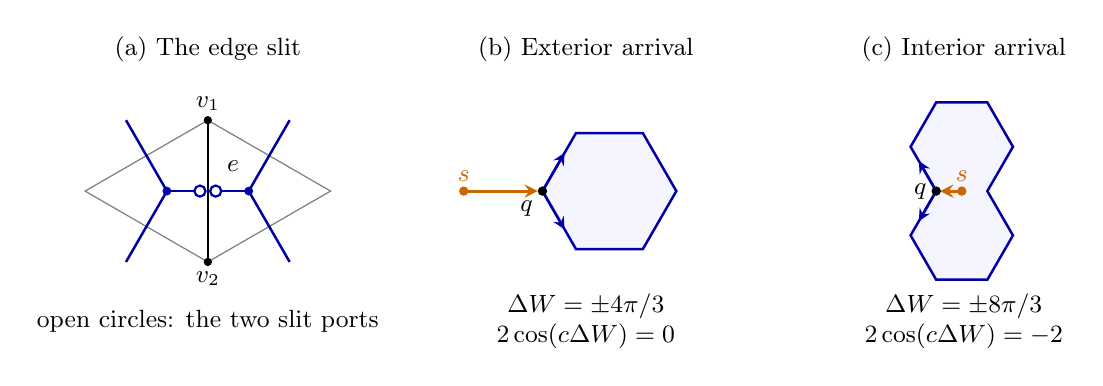
\begin{tikzpicture}[x=1cm,y=1cm,>=stealth,font=\small,
  primal/.style={draw=black!50,line width=.45pt},
  dual/.style={draw=blue!65!black,line width=.9pt},
  arrival/.style={draw=orange!80!black,line width=1.1pt,->}]
\begin{scope}
  \node at (0,1.8) {(a) The edge slit};
  \draw[primal] (0,.9)--(-1.55885,0)--(0,-.9)
                (0,.9)--(1.55885,0)--(0,-.9);
  \draw[black,line width=.7pt] (0,.9)--(0,-.9);
  \draw[dual] (-1.03923,.9)--(-.519615,0)--(-1.03923,-.9)
              (1.03923,.9)--(.519615,0)--(1.03923,-.9);
  \draw[dual] (-.519615,0)--(-.10,0)
              (.10,0)--(.519615,0);
  \fill[blue!65!black] (-.519615,0) circle(1.6pt);
  \fill[blue!65!black] (.519615,0) circle(1.6pt);
  \draw[blue!65!black,fill=white,line width=.8pt]
        (-.10,0) circle(2pt) (.10,0) circle(2pt);
  \fill (0,.9) circle(1.5pt) node[above] {$v_1$};
  \fill (0,-.9) circle(1.5pt) node[below] {$v_2$};
  \node[above right] at (.12,.13) {$e$};
  \node[align=center] at (0,-1.65)
    {open circles: the two slit ports};
\end{scope}
\begin{scope}[xshift=4.8cm]
  \node at (0,1.8) {(b) Exterior arrival};
  \path[fill=blue!4] (-.55,0)--(-.125,.736122)--(.725,.736122)
      --(1.15,0)--(.725,-.736122)--(-.125,-.736122)--cycle;
  \draw[dual] (-.55,0)--(-.125,.736122)--(.725,.736122)
      --(1.15,0)--(.725,-.736122)--(-.125,-.736122)--cycle;
  \draw[dual,->] (-.55,0)--(-.27,.484974);
  \draw[dual,->] (-.55,0)--(-.27,-.484974);
  \draw[arrival] (-1.55,0)--(-.61,0);
  \fill[orange!80!black] (-1.55,0) circle(1.7pt)
      node[above] {$s$};
  \fill (-.55,0) circle(1.7pt) node[below left] {$q$};
  \node[align=center] at (0,-1.65)
    {$\Delta W=\pm4\pi/3$\\$2\cos(c\Delta W)=0$};
\end{scope}
\begin{scope}[xshift=9.6cm]
  \node at (0,1.8) {(c) Interior arrival};
  \path[fill=blue!4] (-.35,0)--(-.675,.562917)--(-.35,1.125834)
      --(.30,1.125834)--(.625,.562917)--(.30,0)
      --(.625,-.562917)--(.30,-1.125834)--(-.35,-1.125834)
      --(-.675,-.562917)--cycle;
  \draw[dual] (-.35,0)--(-.675,.562917)--(-.35,1.125834)
      --(.30,1.125834)--(.625,.562917)--(.30,0)
      --(.625,-.562917)--(.30,-1.125834)--(-.35,-1.125834)
      --(-.675,-.562917)--cycle;
  \draw[dual,->] (-.35,0)--(-.57,.381051);
  \draw[dual,->] (-.35,0)--(-.57,-.381051);
  \draw[arrival] (-.025,0)--(-.30,0);
  \fill[orange!80!black] (-.025,0) circle(1.7pt)
      node[above] {$s$};
  \fill (-.35,0) circle(1.7pt) node[left] {$q$};
  \node[align=center] at (0,-1.65)
    {$\Delta W=\pm8\pi/3$\\$2\cos(c\Delta W)=-2$};
\end{scope}
\end{tikzpicture}
\caption{The slit and the two first-repeat cancellations, with $c=3/8$.
In (a), black and grey segments are primal tiling sides and blue segments
are honeycomb bonds. The bond crossing the side $v_1v_2$ is cut at its
midpoint $e$; the two slit ports are separated slightly for visibility.
Panels (b) and (c) are schematic representatives. The orange leg is
the first prefix arrival at $q$ from the slit source $s$. The path then
traverses the blue cycle and returns to $q$, its first repeated dual
vertex. The two arrows leaving $q$ indicate the two cycle
orientations. Their additional rotations are $\pm4\pi/3$ when $s$ is
outside the cycle and $\pm8\pi/3$ when $s$ is inside. In (c), the arrival
leg occupies the reflex interior sector at $q$.}
\label{fig:slit}
\end{figure}


\begin{lemma}[Slit flux]\label{lem:slit}
For every interior contact $e$,
\[
 T_e=2Z_e+\sqrt2L_e.
\]
Consequently $T_e$ is comparable, with absolute positive constants,
both to the unsigned chord mass through $e$ and to the sum of the
enclosing polygon partition functions at the two endpoints of the
primal tiling side containing $e$.
\end{lemma}

\begin{proof}
First run the finite boundary exploration of Section~\ref{sec:cylinder}
from an outer port, allowing it to stop on the slit. The cancellation
at a previously visited triangle is unchanged. Subtract this flux
identity from the identity without the slit, and sum over all outer
sources. The unchanged outer exits cancel, leaving the chords through
$e$ and the stopped outer-to-slit paths. Reversal changes the sign of
$W$ and preserves its cosine, so
\begin{equation}\label{eq:slit-comparison}
 \begin{split}
 T_e&=\sum_{\gamma\text{ outer-to-slit}}
                x^{m(\gamma)}\cos(cW(\gamma))\\
 &=\sum_{\gamma\text{ slit-to-outer}}
                x^{m(\gamma)}\cos(cW(\gamma)).
 \end{split}
\end{equation}
The last sum uses both slit sources. All explorations are finite, so
this subtraction requires no limiting argument.

Now fix one slit source $s$ and run the same exploration in the
presence of a polygon configuration counted by $Z_e$. Its initial
mass, summed over those configurations, is $Z_e$. At a fresh
unoccupied triangle, extend through either of the other sides. The
two weighted phases sum to one. Stop a branch at an exit, a first
repeated triangle, or the first hit on a gas polygon.

The two first-repeat cases are illustrated in Figure~\ref{fig:slit}.
At a repeated triangle $q$, the two orientations of the resulting
path-cycle have the same positive weight. If the source lies outside
the cycle, their extra rotations after the first prefix arrival at
$q$ are $\pm4\pi/3$, and their phases sum to zero, as in the boundary
exploration. If the source is inside, the prefix arrives from the
interior. The unused third leg is then in the reflex interior sector
of the cycle. For counterclockwise traversal the cycle's turn at $q$
is $-\pi/3$, while the prefix takes turn $+\pi/3$. The two rotations
added after the first arrival are therefore $\pm8\pi/3$, and their
phases sum to
\[
 2\cos(8\pi c/3)=-2.
\]
These terminal terms cancel the first-hit terms for which that cycle
is an independent gas polygon of weight $2x^{|P|}$. The correspondence
keeps all other polygons fixed. Indeed a gas polygon encloses $s$,
so its first hit is from its interior; the prefix before that hit is
disjoint from the polygon and from all remaining gas polygons.
Removing the hit polygon and traversing it in either orientation
gives exactly the two first-repeat branches. Conversely, a first
repeated cycle enclosing $s$ is disjoint from the earlier prefix apart
from its attachment at $q$, and is disjoint from the remaining gas
polygons, so it can be installed as that gas polygon.
The weights agree because the extensions visit each cycle triangle once.

An outer exit cannot coexist with a gas polygon enclosing the slit
source. Let $O_s$ be the real mass of these outer exits, with no gas
polygon present. The remaining slit exits return from the opposite
side of $e$ and close a polygon through $e$. Their total turn is
$\pm2\pi$. With the initial side prescribed, each such marked polygon
is represented once and has real factor
$\cos(2\pi c)=-1/\sqrt2$. Taking real parts in the one-source
conservation identity gives
\[
 Z_e=O_s-\frac{L_e}{\sqrt2},
 \qquad O_s=Z_e+\frac{L_e}{\sqrt2}.
\]
Adding the two slit sources and using \eqref{eq:slit-comparison}
proves the identity.

Let $v_1,v_2$ be the primal vertices at the ends of the side containing
$e$, and let $\mathcal Z^{\Delta_R}_{v_i}$ be their enclosing polygon
partition functions restricted to $\Delta_R$. A dual polygon avoiding
$e$ cannot cross the open primal side, so if it encloses either $v_i$,
it encloses both and also $e$. A polygon through $e$ encloses exactly
one of these vertices, and at most one polygon in a disjoint nest can
pass through $e$. Decomposing by these alternatives gives
\[
 \mathcal Z^{\Delta_R}_{v_1}+\mathcal Z^{\Delta_R}_{v_2}=2Z_e+2L_e,
\]
which is comparable to $2Z_e+\sqrt2L_e$ with absolute positive
constants. Finally, convex boundary flux gives
\[
 \cos(3\pi/8)\sum_{\gamma\ni e}x^{m(\gamma)}
 \le T_e\le\sum_{\gamma\ni e}x^{m(\gamma)}.
\]
This proves the other comparison.
\end{proof}

\subsection{The length numerator and the mean}

Let $A_e$ be the unsigned mass of all ordered boundary chords through
$e$. The planar nesting estimate and Lemma~\ref{lem:slit} give
\[
 A_e\le R^{1/12+o(1)}
\]
uniformly over contacts in the triangle. If $e$ lies in the concentric
triangle of side $R/3$, both adjacent primal vertices have distance
comparable to $R$ from the boundary. For fixed positive
$a_{\rm in},a_{\rm out}$, domain inclusion gives
\[
 \mathcal Z_{v_i}(a_{\rm in}R)
 \le\mathcal Z_{v_i}^{\Delta_R}
 \le\mathcal Z_{v_i}(a_{\rm out}R),\qquad i=1,2.
\]
Monotonicity therefore gives
$A_e=R^{1/12+o(1)}$ uniformly throughout that central region.
The distance from the concentric triangle of side $R/3$ to the
boundary of $\Delta_R$ is $\sqrt3R/9$. Thus every chord through a
central contact has diameter at least $\sqrt3R/9$, and in particular
belongs to $\mathcal C_R(\delta)$ for every fixed $0<\delta\le1/50$.

There are order $R^2$ central contacts and at most order $R^2$
contacts altogether. A path visiting $m$ centres crosses exactly
$m-1$ interior contacts. Define
$M_R(\delta)=\sum_{\gamma\in\mathcal C_R(\delta)}m(\gamma)w(\gamma)$.
For each fixed $0<\delta\le1/50$,
\begin{equation}\label{eq:chord-cutoff-numerator}
 \begin{split}
 M_R(\delta)
 &=Z_R(\delta)+
   \sum_e\sum_{\substack{\gamma\in\mathcal C_R(\delta)\\e\in\gamma}}
        w(\gamma)\\
 &=R^{25/12+o(1)}.
 \end{split}
\end{equation}
The lower bound uses the central contacts, for which all chords are
admissible. The upper bound allows all chords at every contact.
Dividing \eqref{eq:chord-cutoff-numerator} at $\delta=1/100$ by
\eqref{eq:chord-cutoff-denominator} proves the port mean assertion in
Theorem~\ref{thm:triangle}.

We finish with an explicit comparison for ordinary centre walks.
Let $\mathcal W_R(\delta)$ be the ordered centre-to-centre walks
contained in $\Delta_R$, with both endpoints on its inner boundary
layer and diameter at least $\delta R$. If $n(\omega)$ is their number
of edges, put
\[
 \begin{gathered}
 Z_R^\circ(\delta)=\sum_{\omega\in\mathcal W_R(\delta)}x^{n(\omega)},\\
 M_R^\circ(\delta)=
       \sum_{\omega\in\mathcal W_R(\delta)}(n(\omega)+1)x^{n(\omega)}.
 \end{gathered}
\]
Every such walk has at least one extension by boundary half-edges to
two ports, and at most $Q=9$ extensions, since each endpoint triangle
has at most three boundary sides. Deleting the two half-edges recovers
the walk. An extension has exactly $m=n+1$ visited centres and weight
$x^{n+1}=x\,x^n$. Moreover, for an absolute $b$,
\[
 \diam(\omega)\le\diam(\text{port extension})
                 \le\diam(\omega)+b.
\]
Take the two fixed cutoffs $\delta_0=1/100$ and $2\delta_0=1/50$.
For all large $R$, deleting the half-edges from a chord of diameter
at least $2\delta_0R$ leaves a centre walk of diameter at least
$\delta_0R$; every extension of a centre walk at cutoff $\delta_0$
is itself a chord at that cutoff. The weight and multiplicity bounds
give the two squeezes
\begin{equation}\label{eq:centre-cutoff-squeeze}
 \begin{gathered}
 \frac{Z_R(2\delta_0)}{xQ}\le Z_R^\circ(\delta_0)
       \le\frac{Z_R(\delta_0)}x,\\
 \frac{M_R(2\delta_0)}{xQ}\le M_R^\circ(\delta_0)
       \le\frac{M_R(\delta_0)}x.
 \end{gathered}
\end{equation}
Both cutoffs lie in the fixed range already proved. Hence
$Z_R^\circ(\delta_0)\asymp R^{3/4}$ and
$M_R^\circ(\delta_0)=R^{25/12+o(1)}$. Their ratio is the mean of
$n+1$, so the mean edge length is
$M_R^\circ(\delta_0)/Z_R^\circ(\delta_0)-1=R^{4/3+o(1)}$.
This proves the centre-to-centre assertion.

\begin{thebibliography}{99}
\bibitem{BatchelorYung1995}
M.~T.~Batchelor and C.~M.~Yung.
Exact results for the adsorption of a flexible self-avoiding polymer chain
in two dimensions.
\emph{Physical Review Letters} \textbf{74} (1995), 2026--2029.
\href{https://doi.org/10.1103/PhysRevLett.74.2026}
{doi:10.1103/PhysRevLett.74.2026}.

\bibitem{DeConciniProcesi1995}
C.~De Concini and C.~Procesi.
Wonderful models of subspace arrangements.
\emph{Selecta Mathematica, New Series} \textbf{1} (1995), 459--494.
\href{https://doi.org/10.1007/BF01589496}{doi:10.1007/BF01589496}.

\bibitem{DiFrancescoZinnJustin2005}
P.~Di Francesco and P.~Zinn-Justin.
Around the Razumov--Stroganov conjecture: proof of a multi-parameter sum rule.
\emph{Electronic Journal of Combinatorics} \textbf{12} (2005), Research Paper~6.
\href{https://doi.org/10.37236/1903}{doi:10.37236/1903}.
\href{https://arxiv.org/abs/math-ph/0410061}{arXiv:math-ph/0410061}.

\bibitem{DuminilCopinSmirnov2012}
H.~Duminil-Copin and S.~Smirnov.
The connective constant of the honeycomb lattice equals $\sqrt{2+\sqrt2}$.
\emph{Annals of Mathematics} \textbf{175} (2012), 1653--1665.
\href{https://doi.org/10.4007/annals.2012.175.3.14}{doi:10.4007/annals.2012.175.3.14}.

\bibitem{FernandezProcacci2007}
R.~Fern\'andez and A.~Procacci.
Cluster expansion for abstract polymer models. New bounds from an old approach.
\emph{Communications in Mathematical Physics} \textbf{274} (2007), 123--140.
\href{https://doi.org/10.1007/s00220-007-0279-2}{doi:10.1007/s00220-007-0279-2}.

\bibitem{FultonMacPherson1994}
W.~Fulton and R.~MacPherson.
A compactification of configuration spaces.
\emph{Annals of Mathematics} \textbf{139} (1994), 183--225.
\href{https://doi.org/10.2307/2946631}{doi:10.2307/2946631}.

\bibitem{GarbaliNienhuis2017Ground}
A.~Garbali and B.~Nienhuis.
The dilute Temperley--Lieb $O(n=1)$ loop model on a semi infinite strip:
the ground state.
\emph{Journal of Statistical Mechanics: Theory and Experiment} (2017), 043108.
\href{https://doi.org/10.1088/1742-5468/aa6a30}{doi:10.1088/1742-5468/aa6a30}.
\href{https://arxiv.org/abs/1411.7020}{arXiv:1411.7020}.

\bibitem{GarbaliNienhuis2017Sum}
A.~Garbali and B.~Nienhuis.
The dilute Temperley--Lieb $O(n=1)$ loop model on a semi infinite strip:
the sum rule.
\emph{Journal of Statistical Mechanics: Theory and Experiment} (2017), 053102.
\href{https://doi.org/10.1088/1742-5468/aa6bc3}{doi:10.1088/1742-5468/aa6bc3}.
\href{https://arxiv.org/abs/1411.7160}{arXiv:1411.7160}.

\bibitem{GlazmanManolescu2017}
A.~Glazman and I.~Manolescu.
Self-avoiding walk on $\mathbb Z^2$ with Yang--Baxter weights:
universality of critical fugacity and 2-point function.
\emph{Annales de l'Institut Henri Poincar\'e, Probabilit\'es et Statistiques}
\textbf{56} (2020), 2281--2300.
\href{https://doi.org/10.1214/19-AIHP1024}{doi:10.1214/19-AIHP1024}.

\bibitem{Griffiths1976Abel}
P.~A.~Griffiths.
Variations on a Theorem of Abel.
\emph{Inventiones Mathematicae} \textbf{35} (1976), 321--390.
\href{https://doi.org/10.1007/BF01390145}{doi:10.1007/BF01390145}.

\bibitem{GrimmPearce1993}
U.~Grimm and P.~A.~Pearce.
Multi-colour braid--monoid algebras.
\emph{Journal of Physics A: Mathematical and General} \textbf{26} (1993), 7435--7460.
\href{https://doi.org/10.1088/0305-4470/26/24/018}{doi:10.1088/0305-4470/26/24/018}.
\href{https://arxiv.org/abs/hep-th/9303161}{arXiv:hep-th/9303161}.

\bibitem{HammersleyWelsh1962}
J.~M.~Hammersley and D.~J.~A.~Welsh.
Further results on the rate of convergence to the connective constant of
the hypercubical lattice.
\emph{Quarterly Journal of Mathematics} \textbf{13} (1962), 108--110.
\href{https://doi.org/10.1093/qmath/13.1.108}{doi:10.1093/qmath/13.1.108}.

\bibitem{KrachunPanagiotis2026}
D.~Krachun and C.~Panagiotis.
Quantitative sub-ballisticity of self-avoiding walk on the hexagonal lattice.
\emph{Annals of Probability} \textbf{54} (2026), 1109--1125.
\href{https://doi.org/10.1214/24-AOP1730}{doi:10.1214/24-AOP1730}.
\href{https://arxiv.org/abs/2310.17299}{arXiv:2310.17299}.

\bibitem{Li2009Wonderful}
L.~Li.
Wonderful compactification of an arrangement of subvarieties.
\emph{Michigan Mathematical Journal} \textbf{58} (2009), 535--563.
\href{https://doi.org/10.1307/mmj/1250169076}{doi:10.1307/mmj/1250169076}.

\bibitem{Nienhuis1982}
B.~Nienhuis.
Exact critical point and critical exponents of $O(n)$ models in two dimensions.
\emph{Physical Review Letters} \textbf{49} (1982), 1062--1065.
\href{https://doi.org/10.1103/PhysRevLett.49.1062}{doi:10.1103/PhysRevLett.49.1062}.

\bibitem{Penrose1967}
O.~Penrose.
Convergence of fugacity expansions for classical systems.
In T.~A.~Bak (ed.), \emph{Statistical Mechanics: Foundations and Applications},
W.~A.~Benjamin, New York--Amsterdam, 1967, 101--109.

\bibitem{Schoenberg1950PFII}
I.~J.~Schoenberg.
On P\'olya frequency functions. II: Variation-diminishing integral operators of the convolution type.
\emph{Acta Scientiarum Mathematicarum (Szeged)} \textbf{12} (1950), 97--106.
\href{https://acta.bibl.u-szeged.hu/13626/1/math_012_pars_b_097-106.pdf}{Original journal article}.

\bibitem{ScottSokal2005}
A.~D.~Scott and A.~D.~Sokal.
The repulsive lattice gas, the independent-set polynomial, and the Lov\'asz local lemma.
\emph{Journal of Statistical Physics} \textbf{118} (2005), 1151--1261.
\href{https://doi.org/10.1007/s10955-004-2055-4}{doi:10.1007/s10955-004-2055-4}.

\bibitem{ZhouBatchelor1997}
Y.~K.~Zhou and M.~T.~Batchelor.
Critical behaviour of the dilute $O(n)$, Izergin--Korepin and dilute
$A_L$ face models: Bulk properties.
\emph{Nuclear Physics B} \textbf{485} (1997), 646--664.
\href{https://doi.org/10.1016/S0550-3213(96)00654-2}{doi:10.1016/S0550-3213(96)00654-2}.
\href{https://arxiv.org/abs/cond-mat/9611156}{arXiv:cond-mat/9611156}.

\end{thebibliography}
\end{document}
